%& -shell-escape
%\documentclass[a4paper]{aa}
\documentclass[printer]{aa}
% \documentclass{article}
\usepackage[pagebackref,colorlinks,citecolor=blue,urlcolor=blue,linkcolor=blue]{hyperref}
\usepackage[varg]{txfonts}
\usepackage{graphicx}
\usepackage{natbib}
\usepackage{amssymb}
\usepackage{amsmath}
\usepackage{tabularx}
\usepackage{hhline}
\usepackage{makecell}
\usepackage{placeins}
\usepackage{tikz}
\usepackage{subcaption}
\usepackage{lipsum}
\usetikzlibrary{arrows,positioning,shapes} %,optics}
\usepackage{xspace}
\usepackage{mathtools}
\usepackage{{booktabs}}

%\usepackage[squaren,Gray]{SIunits}
\usepackage{siunitx}
%\usepackage{units} % nicefrac
%\newcommand{\units}[1]{$\mathrm{#1}$}

%instrument 
\newcommand{\SD}{StarDICE\xspace}
\newcommand{\Oldthorlabs}{SM05PD1B\xspace}
\newcommand{\Newthorlabs}{SM05PD3A\xspace}
\newcommand{\Qsolar}{Q_{\mathrm{solar}}}
\newcommand{\Qsolarmes}{Q_{\mathrm{solar}}^{\mathrm{mes}}}
\newcommand{\Qsolarcal}{Q_{\mathrm{solar}}^{\mathrm{cal}}}

\newcommand{\Qphot}{Q_{\mathrm{phot}}}
\newcommand{\Qphotmes}{Q_{\mathrm{phot}}^{\mathrm{mes}}}
\newcommand{\Qphotcal}{Q_{\mathrm{phot}}^{\mathrm{cal}}}
\newcommand{\Qphotcont}{Q_{\mathrm{phot}}^{\mathrm{532}}}

\newcommand{\Qccd}{Q_{\mathrm{ccd}}}
\newcommand{\Qccdcal}{Q_{\mathrm{ccd}}^{\mathrm{cal}}}
\newcommand{\Qccdmes}{Q_{\mathrm{ccd}}^{\mathrm{mes}}}
\newcommand{\Qccdcont}{Q_{\mathrm{ccd}}^{\mathrm{532}}}

\newcommand{\Qspectro}{Q_{\mathrm{spectro}}}
\newcommand{\Qspectrocont}{Q_{\mathrm{spectro}}^{\mathrm{532}}}
\newcommand{\Qspectromain}{Q_{\mathrm{spectro}}^{\mathrm{main}}}

\newcommand{\Ssolarstat}{\sigma_{\mathrm{solar}}^{\mathrm{stat}}}
\newcommand{\Sphotstat}{\sigma_{\mathrm{phot}}^{\mathrm{stat}}}
\newcommand{\Qghost}{Q_{\mathrm{ghost}}}
\newcommand{\Rspectro}{R_{\mathrm{spectro}}}
\newcommand{\Rcbp}{R_{\mathrm{CBP}}}
\newcommand{\Rtel}{R_{\mathrm{tel}}}

\newcommand{\Esolar}{\epsilon_{\mathrm{SC}}}
\newcommand{\Espectro}{\epsilon_{\mathrm{spectro}}}
\newcommand{\Espectrocont}{\epsilon_{\mathrm{spectro}}^{\mathrm{532}}}
\newcommand{\Ephot}{\epsilon_{\mathrm{phot}}}
\newcommand{\Ephotcont}{\epsilon_{\mathrm{phot}}^{\mathrm{532}}}
\newcommand{\Eccd}{\epsilon_{\mathrm{ccd}}(\lambda)}

\newcommand{\spinhole}{\SI{75}{\micro\meter}\xspace}
\newcommand{\bpinhole}{\SI{5}{\milli\meter}\xspace}

\newcommand{\mes}{{}_{\mathrm{, \, mes}}}
\newcommand{\cont}{{}_{\mathrm{, \, 532}}}  %cont plutôt que 532 ?
\newcommand{\contcomp}{{}_{\mathrm{, \, comp}}}  %cont plutôt que 532 ?

\newcommand{\Kghost}{K_{G_1/G_0}(\lambda)}
\newcommand{\Kpinholes}{K_\mathrm{\spinhole/\bpinhole}(\lambda)}

\newcommand{\Rwindow}{R_{\mathrm{win}}(\lambda)\xspace}
\newcommand{\Rccd}{R_{\mathrm{ccd}}(\lambda)\xspace}

\newcommand{\bkg}{\mathrm{bkg}}
\newcommand{\Kghostfit}{K_{G/A}}
\newcommand{\Kghostfitfirst}{K_{G_1/A}}

%\newcommand{\Kg_fit}{\mathrm{K_{G_{(1, 2)}/A}}}

\newcommand{\todo}[1]{\textbf{\textcolor{red}{[#1]}}\xspace}
\newcommand{\com}[1]{\textbf{\textcolor{orange}{(#1)}}\xspace}
\newcommand{\up}[1]{\textsuperscript{#1}}
\renewcommand\tabularxcolumn[1]{m{#1}}


\usepackage[outputdir={fig},debug]{dot2texi}
%\usepackage{draftwatermark}
\usepackage{xspace}
%\SetWatermarkText{DRAFT}
%\SetWatermarkScale{6}
%\SetWatermarkLightness{0.9}
\newcommand{\angexp}{\circ{a}}
\newcommand{\texp}{\ensuremath{\tau}\xspace}
\newcommand{\FixMe}[1]{\textbf{\textcolor{red}{[#1]}}\xspace}
\newcommand{\SZF}[1]{\textbf{\textcolor{blue}{[#1]}}\xspace}
\newcommand{\MARC}[1]{\textbf{\textcolor{green}{[#1]}}\xspace}
\newcommand{\THIERRY}[1]{\textbf{\textcolor{green}{[#1]}}\xspace}

\newcolumntype{M}[1]{>{\centering\arraybackslash}m{#1}}
%\renewcommand{\arraystretch}{2}
%\setlength{\arrayrulewidth}{1.25pt}

\graphicspath{{fig/}}
\makeatletter
\newcommand*\ExpandableInput[1]{\@@input#1 }
\makeatother
\DeclareMathOperator*{\med}{med}

\title{The StarDICE absolute flux calibration experiment: Characterisation of the photometric instrument with a collimated beam projector}

\author{
Thierry Souverin\inst{1}
 \and Jérémy Neveu\inst{2,7}
 \and Marc Betoule\inst{1}
 \and Sébastien Bongard\inst{1}
 \and Elana Urbach\inst{7}
 \and Sasha Brownsberger\inst{7}
 \and Christopher W. Stubbs\inst{7}
 \and Pierre Éric Blanc\inst{4}
 \and Johann Cohen Tanugi\inst{5,6}
 \and Sylvie Dagoret-Campagne\inst{2}
 \and Fabrice Feinstein\inst{3}
 \and Delphine Hardin\inst{1}
 \and Claire Juramy\inst{1}
 \and Laurent Le Guillou\inst{1}
 \and Auguste Le Van Suu\inst{4}
 \and Marc Moniez\inst{2}
 \and Bertrand Plez\inst{5}
 \and Nicolas Regnault\inst{1}
 \and Eduardo Sepulveda\inst{1}
 \and Kélian Sommer\inst{5}
}
\institute{
LPNHE, CNRS/IN2P3 \& Sorbonne Université, 4 place Jussieu, 75005 Paris, France
 \and Universit\'e Paris-Saclay, CNRS, IJCLab, 91405, Orsay, France
 \and Aix Marseille Univ, CNRS/IN2P3, CPPM, Marseille, France
 \and Université d’Aix-Marseille \& CNRS, Observatoire de Haute-Provence, 04870 Saint Michel l’Observatoire, France
 \and LUPM, Université Montpellier \& CNRS, F-34095 Montpellier, France
 \and LPC, université Clermont Auvergne, CNRS, F-63000 Clermont-Ferrand, France
 \and Sorbonne Universit\'e, CNRS, Universit\'e de Paris, LPNHE, 75252 Paris Cedex 05, France
}

\abstract{The measurement of Type Ia supernovae magnitudes serves as a mean to access cosmological distances and parameters. Yet, current and upcoming large photometric surveys, including ZTF, DES, HSC and LSST require a substantial improvement in the calibration accuracy of their photometry to reduce systematic uncertainties in cosmological constraints.}{The StarDICE experiment is designed to establish accurate broadband flux references for these surveys, aiming forsub-percent precision in magnitude measurements. This requires a precise measurement of the filter bandpasses of both the StarDICE and survey instruments with sub-nanometer accuracy. To that end, we have developed the Collimated Beam Projector (CBP), an optical device capable of calibrating the throughput of an instrument and of its filter.}{We built a CBP with a tunable laser source and a reversed telescope to emit a parallel monochromatic light beam that is continuously monitored in flux and wavelength. The emitted flux is measured using a large area photodiode, previously calibrated relative to a NIST photodiode. We then measure the StarDICE telescope's throughput and its filter transmissions.}{After carefully analyzing the systematic uncertainties, we have achieved sub-nanometer accuracy in determining filter central wavelengths and detected out-of-band leakages at the \num{e-4} relative level. Furthermore, we have synthesized the equivalent transmission for full pupil illumination from four sample positions in the StarDICE telescope mirror, with an accuracy of approximately \SI{0.2}{nm} for central wavelengths and \SI{7}{mmag} for broadband fluxes.}{These results validate the feasibility of caracterizing a telescope at the required level, and paves the way for future developments, such as a portable CBP versions for in-situ transmission monitoring.}

\begin{document}

\maketitle

%\section{Currently happening}
%
%\begin{itemize}
%\item SC linearity
%\item pinhole choice
%\item dark current caracterization
%\item Photo-diode change
%\end{itemize}

%\tableofcontents

\section{Introduction}

The calibration of optical wide-field surveys needs to reach new levels of precision to meet the requirements of type Ia supernovae (SNe Ia) cosmology. SNe Ia are standard candles, a class of objects with predictable luminosity that are used as probes to characterize dark energy in the late Universe. By measuring the luminosity distance of SNe Ia at different redshifts, we can infer dark energy properties. This luminosity distance is obtained by measuring the maximum amplitude of the SN Ia light curve, which is observed within different optical bands depending on its redshift. Errors in the relative flux calibration between the different bands have a knock-on effect on systematic errors in the Hubble diagram, which are then propagated to dark energy parameters constraints.

Current photometric surveys like the Dark Energy Survey (DES) \citep{Brout_2019} or Subaru Hyper Suprime-Cam (HSC) \citep{hsc_2019} observed hundreds of SNe Ia, and the Zwicky Transient Facility (ZTF) \citep{ztf_2022} should total up to about \num{10000} spectroscopically confirmed SNe Ia, a consequent increase compared to previous surveys. Joint analysis has been performed to benefit from the different existing surveys, reducing the statistical uncertainty on the measurement of cosmological parameters (\citealt{Betoule_2014,Scolnic_2018,Brout_2022,rubin2023union}). Additionally, we expect the SNe Ia catalog to reach a new order of magnitude within the next decade thanks to the Legacy Survey of Space and Time (LSST) undertaken by the Vera Rubin Observatory \citep{lsst}, which is expected to observe between 120,000 and 170,000 SNe Ia up to redshifts $z \sim 0.3$ \citep{lsst_2022}. With this tremendous increase, the statistical uncertainty on cosmological parameters will consequently diminish, leaving the photometric calibration as one major source of systematic uncertainty. Therefore, to benefit from the incoming statistics of the present and future surveys, the photometric calibration needs to reach sub-percent precision.

SNe Ia survey bandpasses are calibrated relatively to the CALSPEC catalog of spectrophotometric standard stars (\cite{Bohlin_2020}), which relies on the radiative transmission model of white dwarf atmospheres (\cite{Narayan_2019}). To transfer this calibration to the photometric survey, it is necessary to take into account two additional components: (i) the terrestrial atmospheric transmission, and (ii) the survey filters transmissions as a function of wavelength, with particular attention given to the bandpasses edges wavelength position. The former can be inferred by airmass regression with observations of CALSPEC reference stars, or by slitless spectrophotometric analysis with a dedicated telescope such as the Rubin Observatory's auxiliary telescope (AuxTel), as detailed in \cite{Neveu_2024}. The latter needs beforehand precise measurements of the bandpasses throughput. Multiple strategies have been developed to provide this measurement on different surveys. The most common approach consists of using calibrated sensors such as the ones supplied by the National Institute of Standards and Technologies (NIST) \citep{houston2008detectors} to monitor a light source used to illuminate a telescope to measure its throughput and filter transmissions. Several approaches involve diffusion on a flat-field screen toward the instrument \citep{stubbs2006,marshall2013}. Other designs have been developed, like \cite{Lombardo_2017} which involves integrating spheres and parabolic mirrors to redirect the light in a parallel beam.

The StarDICE experiment (\citealt{Betoule_2023}) proposes a metrology chain from laboratory flux references toward the measurement of standard star spectra. Several steps are needed to calibrate increasingly sensitive detectors, and finally transfer this calibration to on-sky sources. The StarDICE \SI{40}{\centi\meter} diameter telescope is calibrated with a stable light source positioned far enough (\textasciitilde {\SI{100}{\meter}) to appear as a pointlike source, and provides in-situ calibration of the instrument. Composed of LEDs, the calibrated light will emit broadband flux which will be used to monitor the $ugrizy$ filters of the \SD{} telescope at the millimagnitude level. Beforehand, it is necessary to have a laboratory measurement of the filter transmission at high wavelength resolution to interpret the broadband LED and star measurements. In this context, a Collimated Beam Projector (hereafter CBP) has been developed to accurately measure the StarDICE telescope response $\Rtel(\lambda)$, including the optics, the CCD camera quantum efficiency, and the filter transmission. 

The CBP was originally designed for the LSST telescope (\citealt{ingraham2016}), and prototypes have been used to measure the throughput of the CTIO \SI{0.9}{\meter} telescope and the DECam wide field imager, respectively in \cite{coughlin2018} and \cite{coughlin2016}. Compared to flat-field illumination devices, the CBP is a device able to project monochromatic light in a collimated beam, which provides parallel monochromatic illumination over a portion of the primary mirror. A first prototype of the CBP for StarDICE has been developed in \cite{Mondrik_2023} as a proof-of-concept, and measured the instrument throughput with a precision of \textasciitilde 3\% for wavelengths between \SI{400}{\nano\meter} and \SI{800}{\nano\meter}, and a wavelength calibration estimated at \textasciitilde \SI{0.2}{\nano\meter}. 

This paper details the enhanced version of the StarDICE CBP now equipped with a tunable laser as a monochromatic source, that injects light at the focal point of a Ritchey-Chrétien telescope mounted backwards. The output light of the CBP is collimated and illuminates the StarDICE telescope pupil to measure its throughput. Combining the calibration effort provided by \cite{houston2008detectors} and \cite{solarcell} for the detectors, and all the lessons learned from previous prototypes, we aim at measuring the StarDICE telescope throughput and $ugrizy$ filter transmissions at the sub-percent level. The other goal is to confirm the wavelength calibration accuracy of \SI{0.2}{\nano\meter}. This study has two major intents: (i) to provide a first measurement of the StarDICE filter transmission to contribute to the metrology chain of the experiment, and (ii) to serve as a pathfinder for the future measurement of the LSST telescope with its dedicated version of the CBP.

The following sections of the paper are structured as follows: Section~\ref{sec:setup} presents the laboratory setup of the experiment and gives an overview of the campaign of measurements. Section~\ref{sec:rcbp} details the measurements of the CBP optics response. Section~\ref{sec:rsd} presents the obtained measurements of StarDICE telescope throughput and filter transmissions. The StarDICE full-pupil synthesizing methodology and main results are presented in Section~\ref{sec:pupil_stitching} and discussed in Section~\ref{sec:discussion}.

% The knowledge of the relative transmission of the filters is thus necessary to account for the redshift effect on SNe Ia colors and therefore constrain the dark energy parameters.
%The Collimated Beam Projector (CBP) is a device that measures the transmission of a telescope and its filters. It is composed of a tunable monochromatic laser (Ekspla NT252), that emits light within a range of [350 - 1100] nm, with a resolution of 1 nm and an accuracy of 1 Å. The
%light is injected with an optical fiber into an integrating sphere, whose output is a pinhole of
%variable size, producing a monochromatic, homogeneous and pointlike lightsource. The pinhole
%is set at the focal point of a 152mm Ritchey-Chrétien a mounted backwards, thus providing a
%parallel beam. A photodiode and a spectrograph monitor the surface brightness and wavelength
%of the light inside the sphere. The response of the CBP optical device R CBP (λ) is measured
%by shooting directly into a flux calibrated solar cell 2 , as the ratio of the charges detected in the
%solar cell over the charges detected the monitoring photodiode (fig.2).


\section{Laboratory setup}
\label{sec:setup}

Our setup is composed of three main components: the \SD telescope, a large area photodiode used as a calibration reference, and the CBP which illuminates either one or the other. In the following sections, we will describe each component in detail and explain their operation.

\subsection{\SD}
\label{sec:stardice}

The \SD photometric instrument consists in a Newton
telescope with a primary mirror of \SI{40}{\centi\meter} diameter
(16'') and \SI{1.6}{\meter} focal length ($f/D = 4$). The focal plane
hosts an Andor Ikon-M DU934P-BEX2-DD camera, equipped with a deep
depleted and back-illuminated CCD sensor (E2V DU934P). The active area
of the sensors is
$\SI{13.3}{\milli\meter}\times\SI{13.3}{\milli\meter}$ divided in
$1024\times 1024$ square pixel of \SI{13}{\micro\meter} side. In this
baseline setup, the pixel resolution is \SI{1.68}{\arcsec} and the
field of view $\SI{28.6}{\arcmin}\times\SI{28.6}{\arcmin}$.

A 9-slots \SI{28.5}{\milli\meter} filter-wheel in front of the camera
features 6 interference filters in the $ugrizy$ photometric system, a
Star Analyser 200 diffraction grating, and a \SI{0.2}{\milli\meter}
pinhole. The remaining slot is left empty. Aside the optional filters,
the only other glass part in the light-path is the non-coated
fused-silica window of the CCD cell\footnote{The manufacturer code for
  this window is WN35FS(BB-VV-NR)W}. The two sides of the window are
affected by a \SI{0.5}{\degree} wedge.

The z-position of camera-filterwheel assembly is adjustable over
\SI{9}{\centi\meter} allowing to focus from distances as close as
\SI{35}{m} up to infinity. The 11cm diagonal flat is oversized to
ensure the fully-illuminated plane extends over the sensor with a
comfortable margin in all optical configurations. A model of the
baffling and optics of the instrument build upon the
batoid\footnote{\url{https://github.com/jmeyers314/batoid}} raytracing
software has been tuned on pinhole images and is described in a
companion technical note \cite{}.

In operation, the camera sensor is thermoelectrically cooled-down to a
temperature of \SI{-70}{\celsius}, delivering a median dark-current of
\SI{0.15}{e^-/s}, neglected for the $\sim 1s$ exposures considered in
this study. When operated in the lab, the telescope was mounted on a
custom altazimutal mount to enable easy alignment with the CBP.

\subsection{Collimated Beam Projector}
\label{sec:cbp}

The Collimated Beam Projector (CBP) general setup needs the following: one tunable monochromatic light source, and an optic device able to recreate a parallel beam from a point source. 
In our case, the light source is an Ekspla NT252 tunable laser, using a Q-switched pump laser at \SI{532}{\nano\meter} and non-linear crystals to produce powerful monochromatic pulses from 335 to \SI{2600}{\nano\meter}. The pulse duration is fixed and lies between 1 to \SI{4}{\nano\second} with an energy of \SI{1.1}{\milli\joule} in the near infra-red. The energy can be decreased at will by a factor of 2 using the tuning of the Q-switch (namely QSW in the following) which degrades the quality factor of the resonant cavity. The pulses are shot with a fixed frequency of \SI{1}{\kilo\hertz} and can be shot in two modes. The first one is said "continuous", so it shoots pulses in a continuous way. The second one send packets of pulses by "bursts". Each burst is composed from 1 to 1000 pulses, meaning the duration of a burst is restrained between \SI{1}{\milli\second} to \SI{1}{\second}. The pulses have a maximum linewidth below \SI{10}{\per\cm}, which can be converted into a maximum spectroscopic width below \SI{0.4}{\nano\meter} around \SI{600}{\nano\meter}. This is an upper limit quoted by the manufacturer, but measurements taken using a similar laser show bandwidths going from \SI{0.08}{\nm} to \SI{0.48}{\nm} in the 350 to \SI{1100}{\nm} range \citep{woodward2018}. The standard deviation of pulse energy is around 2.5\%. This laser is composed of three stages to operate (from 335 to \SI{669}{\nano\meter}, from 670 to \SI{1064}{\nano\meter} and above \SI{1064}{\nano\meter}), which results in three different regimes of power and light contamination in the CBP. This laser was chosen for the offered wide wavelength range and the high pulse energy, as source power is an important criteria for the CBP calibration with the solar cell. 

The laser output is purified with a diaphragm and a filter wheel. The latter contains three different broad bandpass filters that helps purifying the laser light from pump photons or other resonances in the system. In particular, we use a pass-blue filter BrightLine Multiphoton FF01-680/SP-25 in the regime 530 to \SI{645}{\nano\meter} to remove \todo{a bien justifier}, a pass-red filter RazorEdge LP03-532RU-25 to filter the \SI{532}{\nano\meter} pump photons in the regime 645 to \SI{1074}{\nano\meter}, and a pass-infrared filter RazorEdge LP02-1064RU-25 above \SI{1074}{\nano\meter} to filter $<\SI{1064}{\nano\meter}$ photons appearing in this regime. A black metallic box encloses the entire optical stage to minimize light scattering in the room.

The light is then injected into an optical fiber Thorlabs MHP910L02 of with a wide core diameter of \SI{910}{\micro\meter}, which is plugged into an IS200-4 $\Phi$2'' integrating sphere from Thorlabs, which has an internal \SI{50}{\mm} diameter and is composed of 1 input and 4 output ports. The integrating sphere dilutes the laser flux and breaks the light coherence. Two monitoring instruments are plugged on the sphere. First a silicon photodiode Thorlabs SM05PD3A with a high efficiency in the UV is mounted on an output port orthogonal to the laser input port to control the laser power stability. It is mounted behind a pinhole to reduce the photon flux and ensure that it works in its linear regime. It is read by a Keithley 6514 electrometer at a rate of \SI{0.02}{\second}. We also plug an OceanOptics Q65000 fiber spectrometer on another output to monitor the true laser wavelength and the spectral purity. One port is left free to plug a calibration lamp to calibrate the spectrograph when needed. Finally, a slider with pinholes of different diameters is mounted on the last output port. Figure \ref{fig:sphere} shows a schematic of the integrating sphere and the instruments plugged into it.

In this paper, we used three different pinholes, of diameter \SI{75}{\micro\meter}, \SI{2}{\milli\meter} (respectively P75HK and P2000HK from Thorlabs) \SI{5}{\milli\meter} (homemade). The \SI{5}{\mm} pinhole is the largest possible given the \SD field of view and gives the maximum flux. The other pinholes are used for systematic checks and filter edge analysis. The pinhole slider is attached to the ocular of a 154/1370 Ritchey-Chrétien Omegon telescope, mounted on a robotic Celestron NexStar Evolution 6, in order to position the pinhole at the focal point of the optics. An iris diaphragm is positioned \SI{16}{mm} after the pinhole and adjusted to cut light that would otherwise miss the secondary mirror of the telescope. A small amount of light scatters on the iris blades and is best observed in telescope images of the CBP taken with the \SI{2}{mm} pinhole configuration. In these images, it forms a faint ring with a radius of approximately \SI{340}{pixels}, discinct from the main spot. When comparing annular photometry of the ring to that of the main spot, the fraction of scattered light is usually smaller than \num{6e-4} between 400 and \SI{900}{nm}.

\begin{figure}
    \centering
    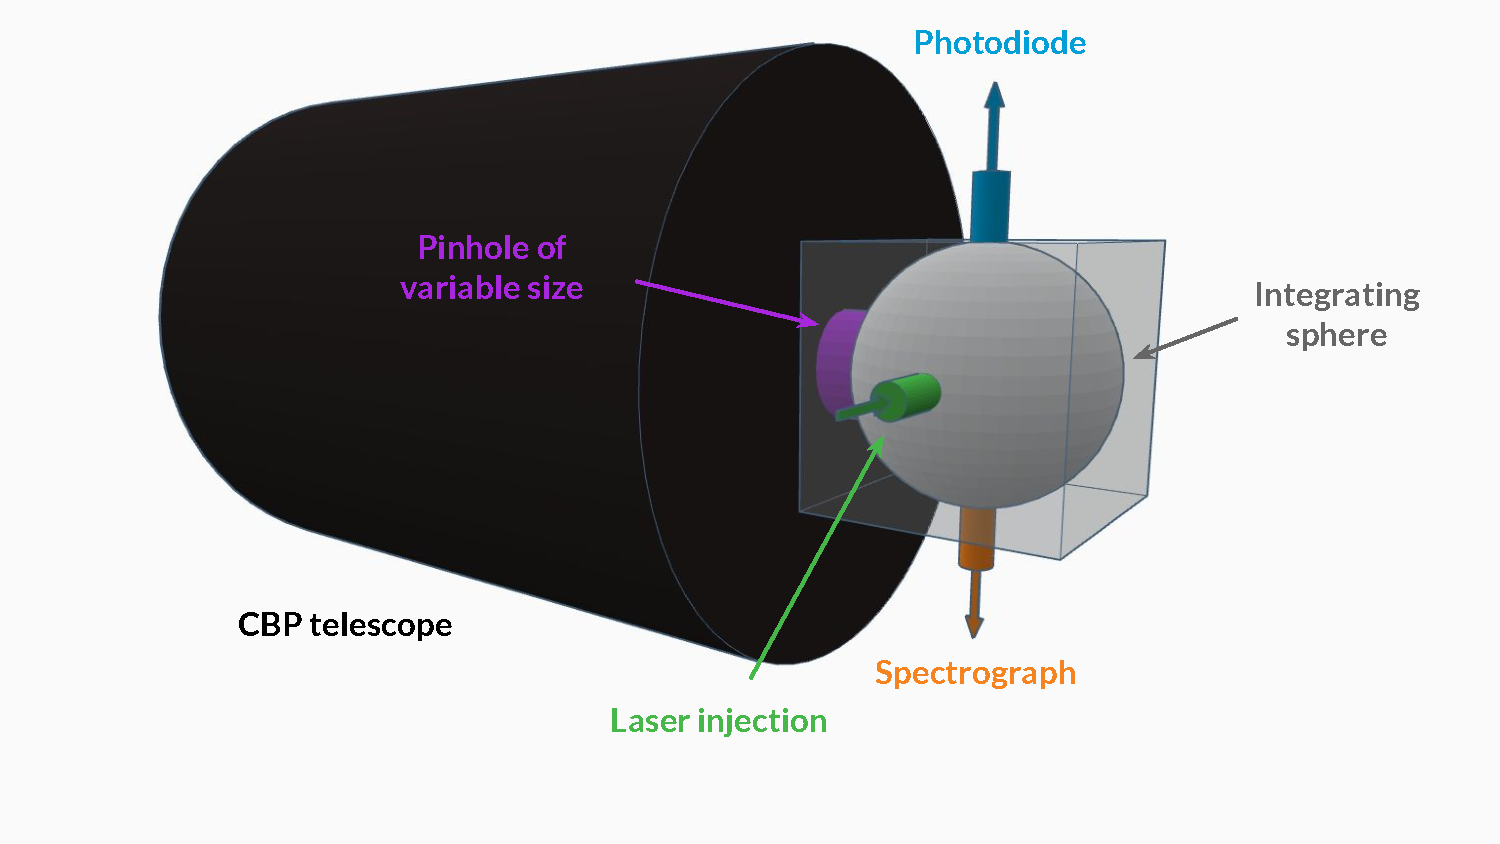
\includegraphics[width=1\columnwidth]{fig/integrating_sphere_3d.pdf}
    \caption{Schematic of the integrating sphere}
    \label{fig:sphere}
    %Tinkercad
\end{figure}


One important improvement in our CBP design compared with \cite{Mondrik_2023} is the use of a solar cell to calibrate and monitor the CBP optical transmission between the optical sphere and the telescope output. It was chosen to have high quantum efficiency and a large shunt resistance. Hence we have a C60 solar cell of 3$^{\mathrm{rd}}$ generation from Sunpower. This solar cell is set on a two-axis mount, one that allows a movement in the direction of the optical axis of the CBP telescope, and another axis that is vertical, which allows to adjust the height of the solar cell. It is placed at \SI{16}{\cm} approximately from the telescope aperture. This solar cell is connected via a coaxial cable to a Keysight B2987A electrometer, the same that was used for its calibration. The charges are measured at a rate of \SI{0.002}{\second}. In Figure~\ref{fig:cbp_setup} right, we show a picture of the setup when the CBP is aiming at the \SD telescope described in section~\ref{sec:stardice}. While a large CBP output beam allows for a larger scan of the telescope mirror, its calibration needs for it to be fully contained by the calibrating sensor. The largest accurate sensor we managed to setup for this experiment is a square solar cell of \SI{12.5}{\centi\meter} width, which thus sets the maximum size of the CBP beam. We adjust the output of the Richey-Chrétien Omegon to that size by cropping it with a frame shaped as a quarter of a disk corresponding to a quadrant of its secondary mirror spider. 

To synchronise the laser and the two electrometers on the same clock, their output trigger lines are plugged in a digital analyser that defines the timestamps for all our data sets. This was a crucial element in the chain to achieve an accurate calibration of the CBP response when signal-to-noise ratio was too low in the solar cell depending on the laser regime.

\begin{figure*}[ht]
\centering
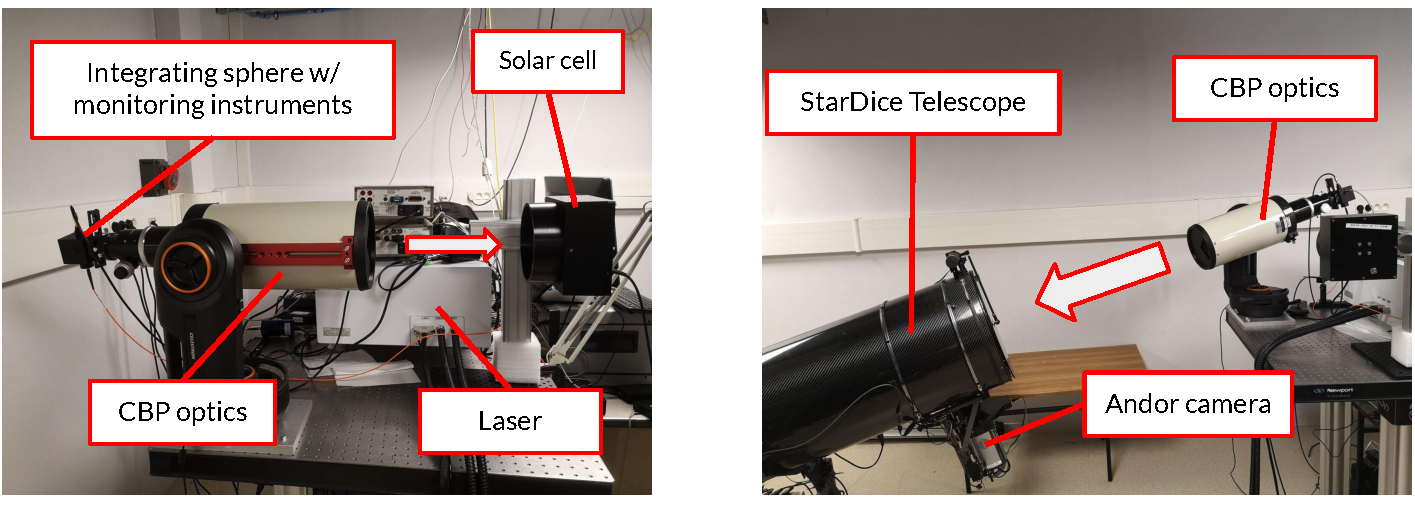
\includegraphics[width=\textwidth]{fig/cbp_setup_cropped.pdf}
\caption{Pictures of the different CBP setups. Left: CBP setup when shooting in the solar cell. Right: CBP setup when shooting in the \SD telescope.}
\label{fig:cbp_setup}
\end{figure*}

In summary, the design of the CBP has undergone several modifications since its initial description in \cite{Mondrik_2023}. Three notable changes include: (1) replacing the laser light source from NIST with an EKSPLA NT 252, which has a slightly different wavelength power cutoff; (2) adding a filtering system to prevent laser harmonics from being injected into the light beam; and (3) incorporating calibration and monitoring of the CBP transmission as part of the instrumentation and observation procedure. This is now done using a solar cell instead of relying on external measurements in a separate experimental setup.


\subsection{Solar cell description}

\subsubsection{Quantum efficiency measurement}
 
The quantum efficiency (QE) as a function of wavelength for the solar cell was measured relative to a NIST-calibrated photodiode by using a monochromator as a light source and using an electrometer to measure the current of the solar cell and of the photodiode at each wavelength. The monochromator wavelength was calibrated with a spectrometer relative to a mercury calibration source. Details of the setup are discussed in ~\cite{solarcell}. The quantum efficiency of the solar cell used for these measurements is shown in Fig.~\ref{fig:qe}. \todo{Comment on the origin of the glitch around 550nm and what has been done to get rid of it} The uncertainty cited is from the standard error of the current measurements.

\begin{figure}[!h]
\centering
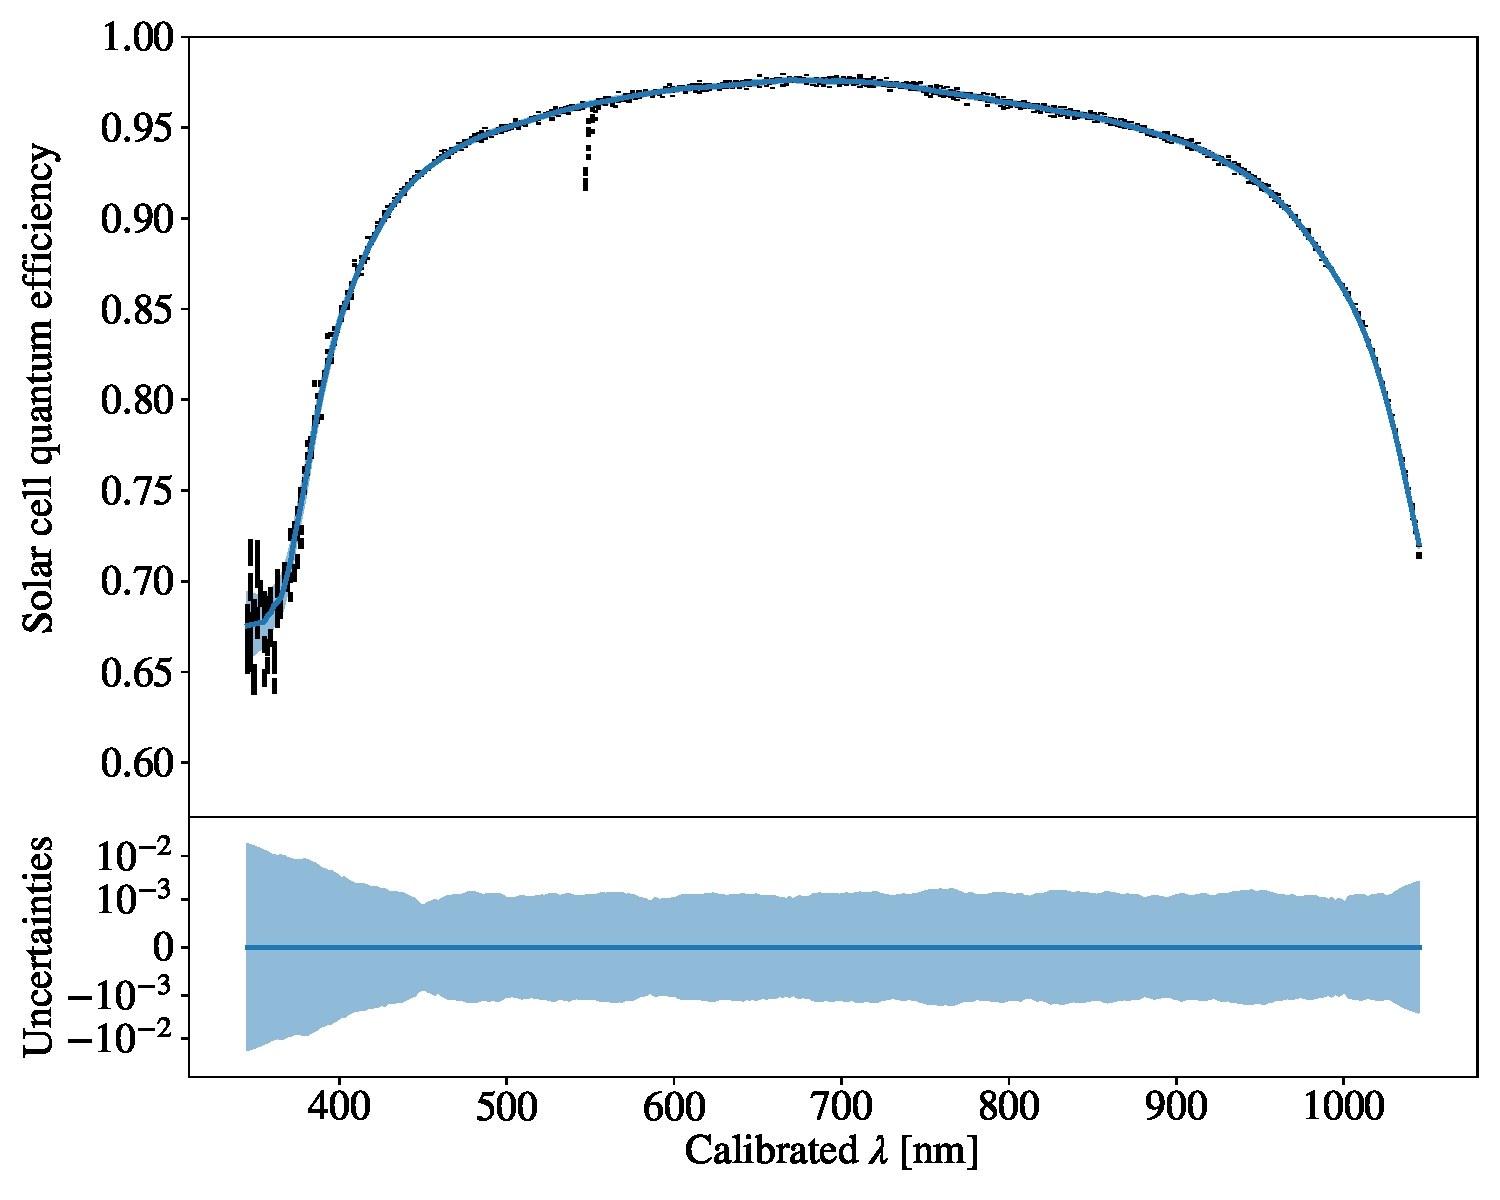
\includegraphics[width=\columnwidth]{solarcell_qe}
\caption{Solar cell quantum efficiency with respect to wavelength (top) and error bar sizes (bottom).}
\label{fig:qe}
\end{figure}

To determine the effect of temperature on QE, the QE of the solar cell was measured as it was heated. At longer wavelengths, the QE increased slightly as the temperature increased (see Fig.~\ref{fig:SC_temp}). This trend is consistent with the temperature dependence of silicon's QE \citep{Green_2008}. At 1050 nm, the QE changes by more than 0.1 percent per degree.
\begin{figure}[!h]
\centering
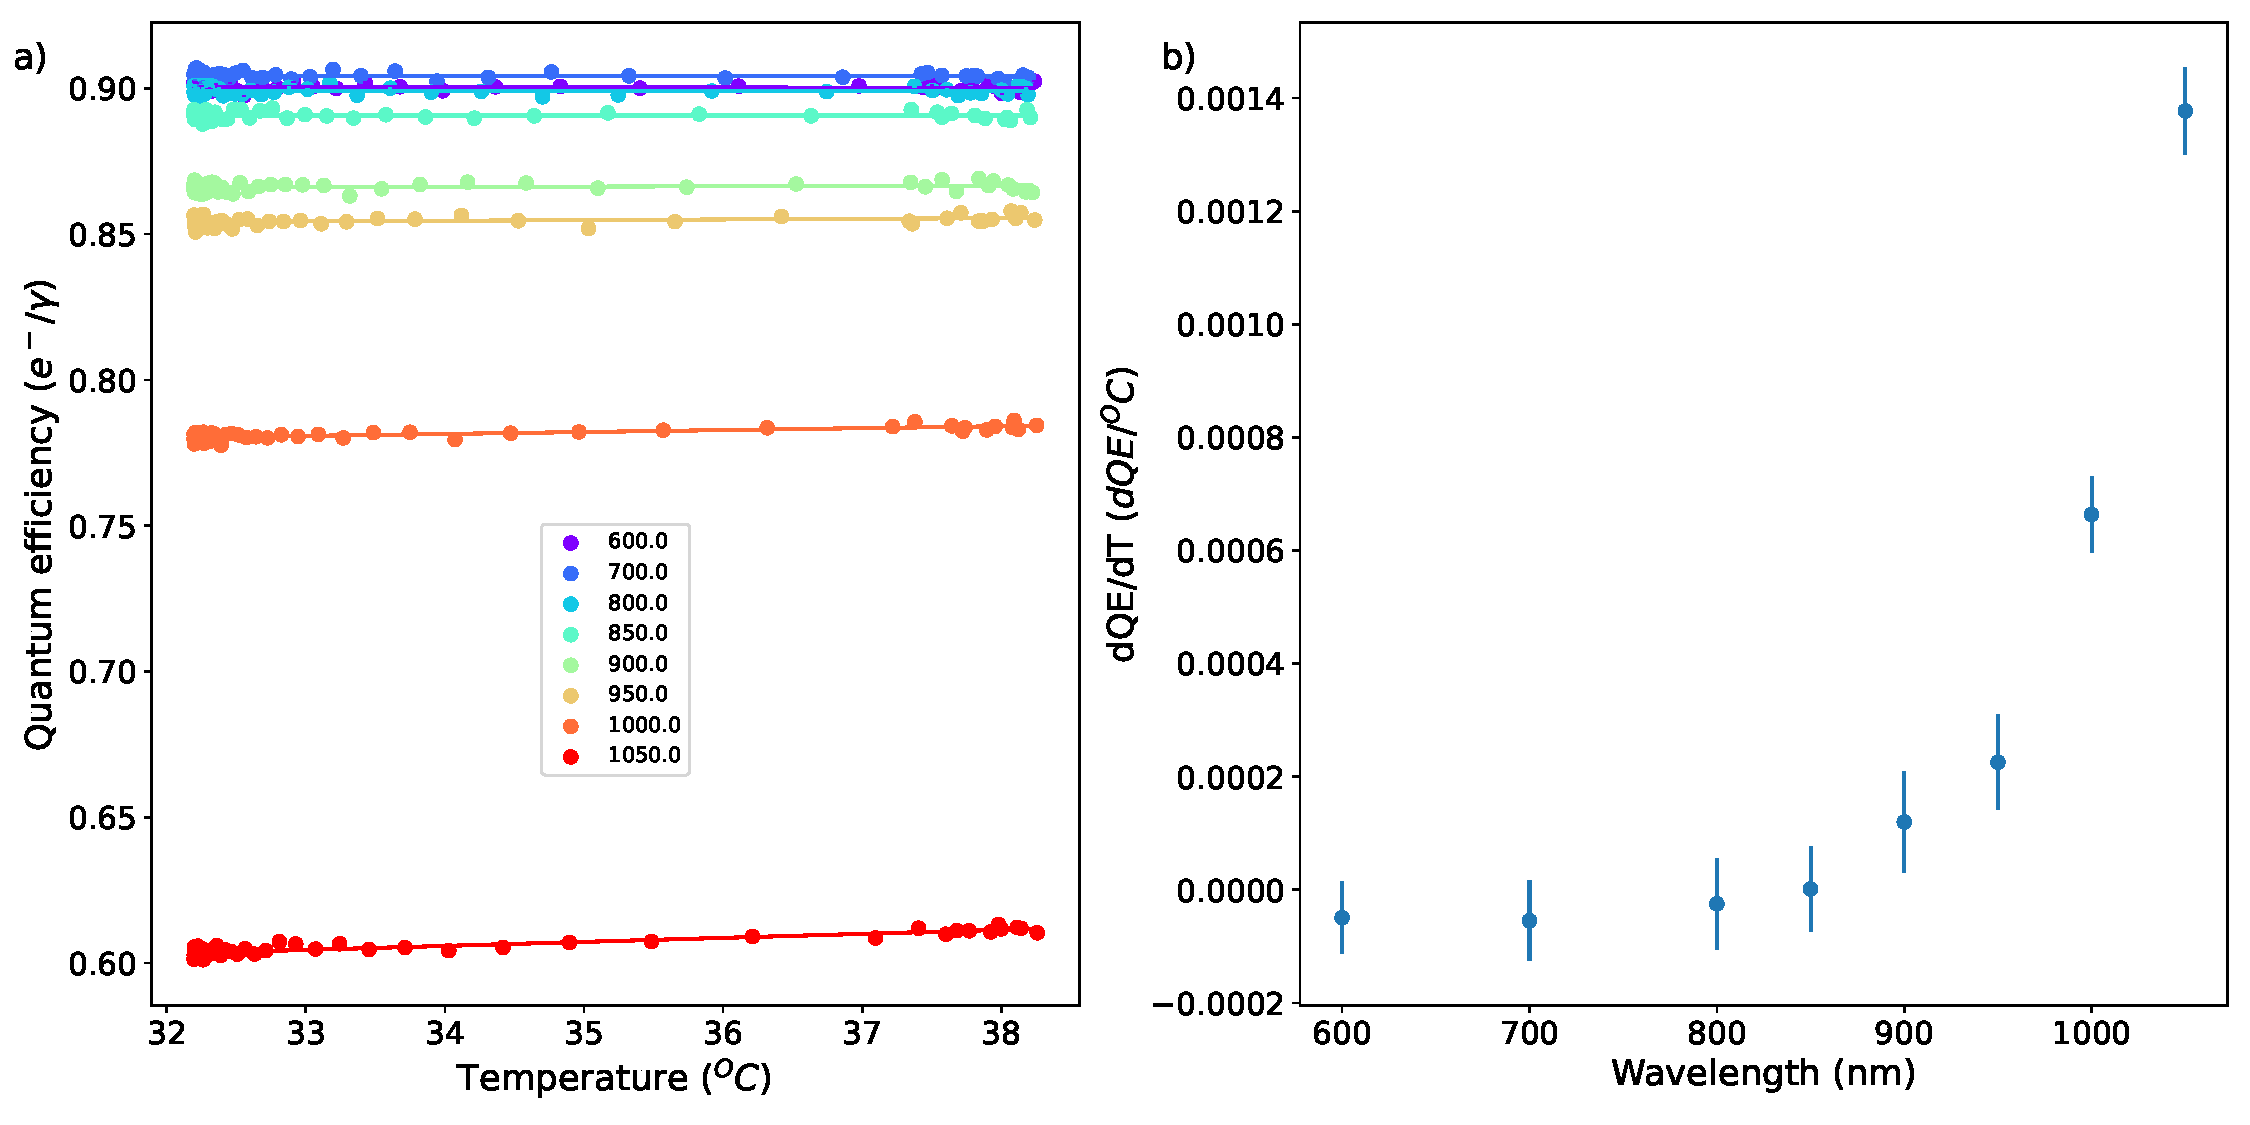
\includegraphics[width=\columnwidth]{SC_temp_dep.pdf}
\caption{(a) Solar cell quantum efficiency vs temperature for wavelengths ranging from 600 to 1050 nm. (b) Fitted change in quantum efficiency per degree Celsius for wavelengths ranging from 600 to 1050 nm.}
\label{fig:SC_temp}
\end{figure}

Additionally, the effect of the angle of incidence on the solar cell QE was measured. The solar cell was rotated up to 35 degrees off-axis. The results are shown in Fig.~\ref{fig:SC_angle}. There is a stronger dependence on angle of incidence at wavelengths that are less than 600 nm, but the change in QE for wavelengths greater than 400 nm is less than 5e-4 per degree.
\begin{figure}[!h]
\centering
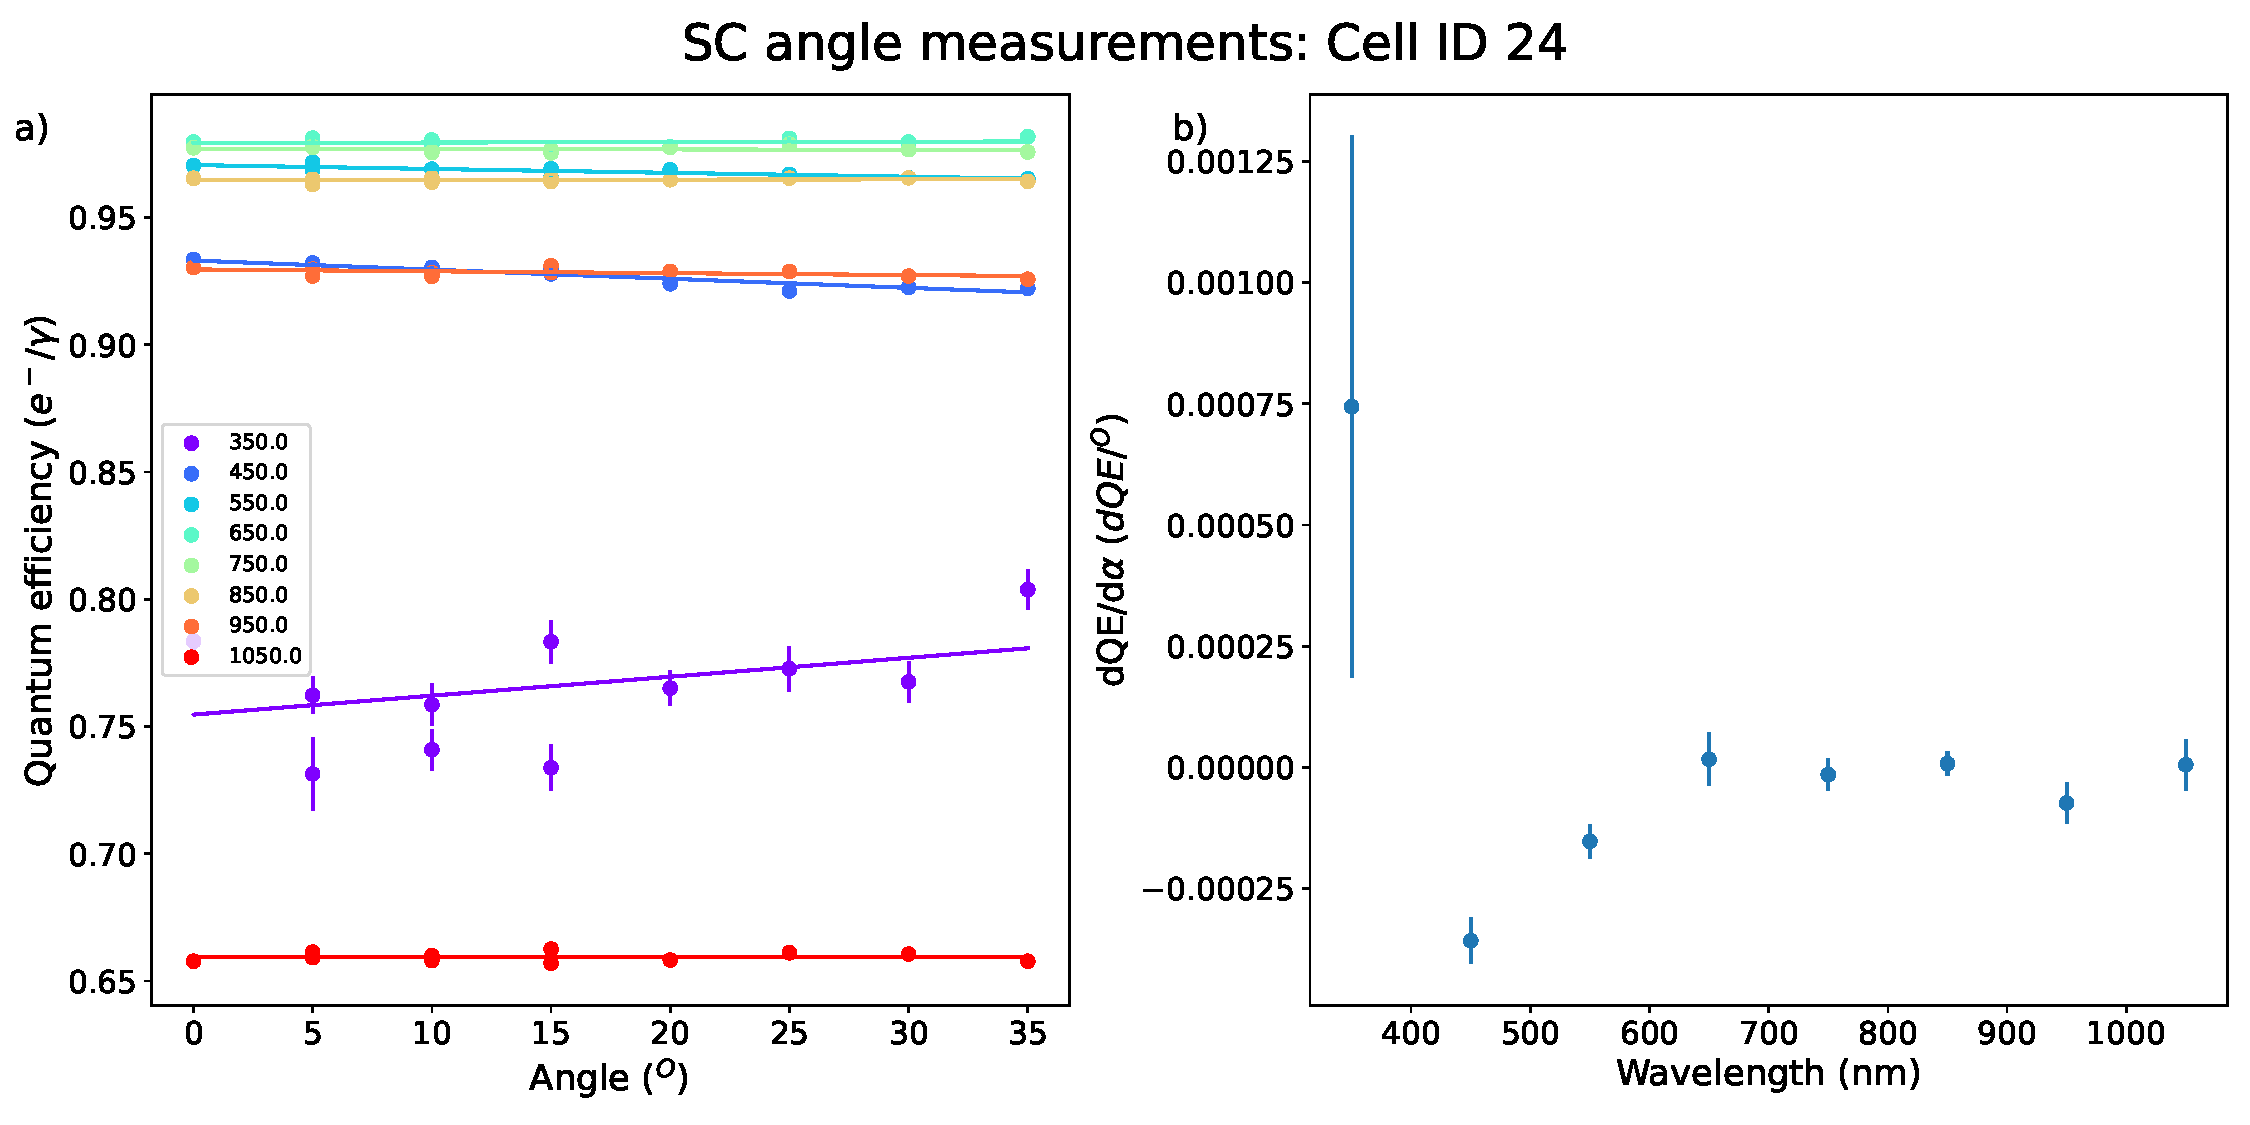
\includegraphics[width=\columnwidth]{SC_angle_dep.pdf}
\caption{(a) Solar cell quantum efficiency vs solar cell tilt relative to normal incidence for different wavelengths. (b) Fitted change in quantum efficiency per degree of solar cell tilt relative to normal incidence vs wavelength.}
\label{fig:SC_angle}
\end{figure}

The solar cell was aligned perpendicalular to the CBP output beam with a precision better than \SI{1}{\degree} and not moved during all the measurement campaign. Meanwhile, room temperature was monitored and has not varied more than \SI{2}{\degreeCelsius}.
%Considering measured variations of quantum efficiency with angle and temperature, we assumed that this systematic is well below the per-mill level and is not considered in the following of the paper. 

%\subsubsection{Current or charge mode}
%
%The charges in the photodiode and the solar cell are read with electrometers in charge mode. This mode is better than the current mode as the integration is performed in a capacitance. This avoids modeling the precise current timelines before integrating them numerically, as they are subtlety different from squarewave functions due to different time responses in the system and contaminated by random dark current fluctuations. 

%\begin{itemize}
%\item Ekspla NT252 tunable laser
%\item Light injection system with filters
%\item Optical sphere ref
%\item Ocean QE65000 spectrograph
%\item Photodiode + Keithley 6514. Fig \ref{fig:thorlabs_response}\\
%  \emph{Old one} (used in summer 2021 up to 14th of October 2021): Thorlabs
%  SM05PD1B with FDS100 spectral response data\\
%  \emph{New one} (replaced on the 14th of October 2021): Thorlabs SM05PD3A with
%  FD11A spectral response data

%\item Pinhole slider
%\item Telescope: Ritchey Chretien Omegon telescope\\
%  Apperture ratio $f/9$\\
%  Apperture $154 mm$ \\  
%\item Telescope mount
%\item Solar Cell on movable mount
%\item Keysight B2987A: in order to be able to chop the light at a higher frequency
%  than what the Keithley can do. And it is a more contemporary instrument.
%\end{itemize}
  
%\begin{figure}[!ht]
%    \begin{center}
%      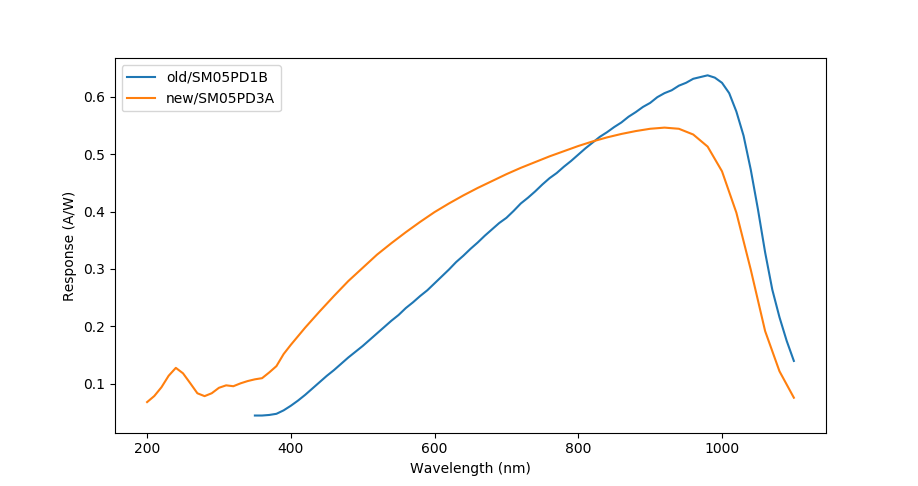
\includegraphics[width=0.8\columnwidth]{thorlabs_response}
%    \end{center}
%    \caption[]{Response curves of the photodiodes. We see the noticeable
%      improvement in the blue for the new one.}
%    \label{fig:thorlabs_response}
%\end{figure}

\subsubsection{Dark current characterisation}

Due to the low resistance of the solar cell, when plugged into the Keysight electrometer we observed a quite strong current even in dark conditions (about \SI{20}{\nano\ampere}). Therefore, we built a device that uses a precision voltage source with a tunable voltage divider to inject a counter-current that cancels this contribution. The current value was tuned to observe approximately no drift when using the Keysight in charge mode inside the usual acquisition time window ($< \SI{1}{\minute}$). Doing so, we avoided saturating the electrometer when using the solar cell in dark and laser-on conditions. 

%\begin{itemize}
%\item Without offset box: $\sim 20 nA$
%\item With offset box: $~ <0> nA \pm 5 nA$
%\end{itemize}
After cancelling the dark current drift, the analysis of the solar cell dark signal revealed a $1/f$ noise, with power line harmonics contributions at \SI{50}{\hertz},  \SI{100}{\hertz}, and \SI{150}{\hertz} (see Figure~\ref{fig:darkcurrentspectrum}). To investigate the source of the $1/f$ component in the power spectrum, we compared the output of the Keysight when connected to a resistor with the same value as the shunt resistance of the solar cell. We found that the two power spectra were identical, leading us to conclude that the fluctuations in the transimpedance amplifier bias voltage are the source of this $1/f$ noise. These fluctuations cause parasitic current to flow through the load resistance. By increasing the load resistance, we can decrease the amplitude of the resulting noise. We therefore chose the calibrated solar cell with the highest shunt resistance we had ($R_{\rm shunt} = \SI{1.8}{\kilo\ohm}$) and limited the burst durations to at most 200 pulses (\SI{200}{\ms}). Doing so, in the burst time window, the Keysight noise is dominated by the power line harmonics whereas the random $1/f$ noise remains subdominant.

%cbp_paper_plots.py
\begin{figure}[h]
\begin{center}
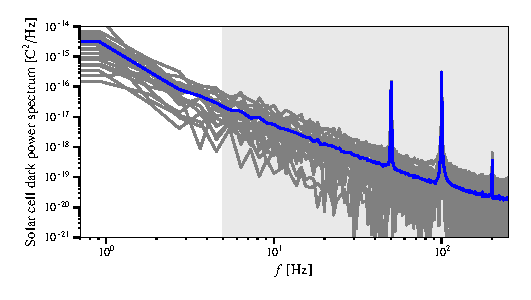
\includegraphics[width=1\columnwidth]{sc_dark_ps}
\end{center}
\caption[]{Solar cell dark current power spectrum for 20 runs without light in the solar cell (gray curves) and their average (blue). The light gray region encompasses expected noise spectrum contribution for \SI{200}{\ms} laser bursts.}
\label{fig:darkcurrentspectrum}
\end{figure}

\FloatBarrier   

\subsection{Equations}

Table~\ref{tab:quantities} sum up the three quantities that are measured with the two setups in Figure~\ref{fig:cbp_setup}.

\begin{table}
  \centering % used for centering table
  \caption{Definition of measured quantities in our \SD+CBP setup.}
    \begin{tabular}{M{1cm} M{7cm}} % centered columns (4 columns)
        \hline\hline % inserts double horizontal lines
        Name & Description \\
        \hline
        \bf{$\Qphot(\lambda)$} & The charge per burst collected by the integrating sphere monitoring photodiode, measured by the Keithley 6514 in Coulomb \\

        \bf{$\Qsolar(\lambda)$} & The charge per burst collected by the solar cell, measured by the Keysight 2987A in Coulomb \\
        \bf{$\Qccd(\lambda)$} & The charge collected by the Andor CCD camera of the \SD telescope in ADU. \\
        \hline %inserts single line
    \end{tabular}
    \label{tab:quantities} % is used to refer this table in the text
\end{table}

First, we need to measure the response of the CBP optics $\Rcbp(\lambda)$ by shooting into the calibrated solar cell as shown in Figure~\ref{fig:cbp_setup} left. It is computed with the Equation~\ref{eq:rcbp}. In this equation, we know the quantum efficiency of the solar cell $\Esolar$ from \cite{solarcell}, and $e$ is the elemental charge of the electron.

\begin{equation}
    \Rcbp(\lambda) = \frac{\Qsolar(\lambda)}{\Qphot(\lambda) \times \Esolar \times e}.
    \label{eq:rcbp}
\end{equation} 

Once we have this response, we can shoot inside the \SD telescope as show in Figure~\ref{fig:cbp_setup} right, and obtain $\Rtel(\lambda)$ with the Equation~\ref{eq:rsd}.

\begin{equation}
    \Rtel(\lambda) = \frac{\Qccd(\lambda)}{\Qphot(\lambda) \times \Rcbp(\lambda)}.
    \label{eq:rsd}
\end{equation}

We will focus on $\Rcbp(\lambda)$ and $\Rtel(\lambda)$ respectively in sections \ref{sec:rcbp} and \ref{sec:rsd}.

\subsection{Strategy}
\label{sec:strategy}

The schedule for all measurements conducted to determine $\Rtel(\lambda)$ and estimate associated systematic uncertainties is outlined in Table\ref{tab:schedule}. Each row in the table corresponds to a specific hardware configuration and measurement run. We have assigned labels to each run and specified the following details: (1) the target of the CBP, (2) the pinhole used in the CBP slide, (3) the QSW setting for the laser, (4) the filters used in the \SD camera filter wheel (when applicable), (5) any specificities of the measurement, and (6) the number of runs.

The campaign of measurement has started and ended with a calibration of the spectrograph. A calibration Hg-Ar lamp was plugged into the integrating sphere and its light was measured with the spectrograph. This corresponds to lines No.~1 and No.~13 of the Table~\ref{tab:schedule}.

Two different pinholes in the CBP slides were used for these measurements. When shooting into the \SD telescope, the \spinhole pinhole forms a point-like image of about 10 pixels in diameter well suited for photometry while avoiding issues related to ghosting. When shooting into the solar cell, the \bpinhole pinhole is necessary to achieve good signal-to-noise ratio. Since $\Rcbp(\lambda)$ depends slightly on the pinhole diameter, we also need to intercalibrate the two responses $R_\mathrm{CBP}^{\mathrm{\SI{5}{\milli\meter}}} (\lambda)$ and $R_\mathrm{CBP}^{\mathrm{\SI{75}{\micro\meter}}} (\lambda)$. This intercalibration can be performed thanks to the measurements in line No.~8 of Table~\ref{tab:schedule}.

A major issue with the CBP is that its output light does not illuminate the entirety of the \SD primary mirror as an astrophysical source would do, but only a portion of it. It is necessary to perform a \textit{pupil stitching} to reconstruct the transmission of the mirror, by combining the measurement of $\Rtel(\lambda)$ when shooting at different positions on the mirror. When doing so, only the point of impact on the mirror is modified, but the point of incidence on the focal plane is the same. The different positions are shown in Figure~\ref{fig:8_mirror_positions}. The pupil stitching corresponds to lines No.~2 and No.~3 of Table~\ref{tab:schedule}. The method used to perform the pupil stitching is detailed in Section~\ref{sec:pupil_stitching}.

To check the uniformity of the \SD focal plane, a measurement of $\Rtel(\lambda)$ at 16 different positions on the focal plane has been performed. The positions are shown in Figure~\ref{fig:ccd_grid}. Only the position on the focal plane is modified while the point of impact on the mirror stays the same. This dataset corresponds to the line No.~12 of Table~\ref{tab:schedule}. 

Finally, some systematic measurements have been carried out. A cap has been placed on the CBP output to measure the background of the room for both setup configurations, corresponding to lines No.~9 and No.~10 of Table~\ref{tab:schedule}. A measurement of the scattered light is possible with the dataset No.~11, by shifting the position of the solar cell from the CBP output of approximately \SI{16}{\centi\meter}.


\begin{table*}[t]{}
  \centering
  \caption{Detailed schedule of the measurements.}
    \begin{tabular}{M{.25cm} M{2.25cm} M{1.75cm} M{1.1cm} M{1.75cm} M{3cm} M{3.5cm} M{1.25cm}}
        \hline\hline
         \bf{N$^{\circ}$} & \bf{Label} & \bf{Target} & \bf{Pinhole} & \bf{QSW} & \bf{\SD bands} & \bf{Specitifity} & \bf{Number of runs} \\ 
         \hline
         1 & Wavelength calibration & Spectrograph & - & - & - & Hg-Ar lamp used for light source & 1 \\ 
         
         2 & Radial pupil stitching & \SD & \SI{75}{\micro\meter} & MAX & \shortstack{u, g, r, i, z, y, \\ EMPTY, GRATING} & 4 radial positions on the mirror  & 1 per position \\
         
         3 & Quadrant pupil stitching & \SD & \SI{75}{\micro\meter} & MAX & EMPTY & 4 quadrant positions on the mirror  & 1 per position \\
         
         4 & Repeatability measurement & \SD & \SI{75}{\micro\meter} & MAX & \shortstack{u, g, r, i, z, y, \\ EMPTY, GRATING} & Same position on the mirror and focal plane for \SI{75}{\micro\meter} pinhole & 3 \\
         
         5 & CBP response calibration before & Solar cell & \SI{5}{\milli\meter} & 298, MAX & - & Monitor the CBP response before the \SD measurement & 5 \\
         
         6 & \SD main calibration & \SD & \SI{5}{\milli\meter} & MAX & \shortstack{u, g, r, i, z, y, \\ EMPTY, GRATING} & Same position on the mirror and focal plane for \SI{5}{\milli\meter} pinhole & 5 \\
                  
         7 & CBP response calibration after & Solar cell & \SI{5}{\milli\meter} & 298, MAX & - & Monitor the CBP response after the \SD measurement & 5 \\
         
         8 & Pinholes inter-calibration & \SD & \SI{75}{\micro\meter}, \SI{2}{\milli\meter}, \SI{5}{\milli\meter} & MAX & EMPTY & 3 different pinhole sizes & 1 per pinhole \\
            
         9 & \SD background measurements & \SD & \SI{5}{\milli\meter} & MAX & EMPTY & Cap on CBP output to block the light & 1 \\
            
         10 & Solar cell background measurements & Solar cell & \SI{5}{\milli\meter} & MAX & - & Cap on CBP output to block the light & 2 \\
            
         11 & Solar cell distance calibration & Solar cell & \SI{5}{\milli\meter} & 298, MAX & - & 2 solar cell positions at \SI{16}{\centi\meter} relative distance & 1 per position \\
            
         12 & Focal plane measurement & \SD & \SI{75}{\micro\meter} & MAX & EMPTY & 4x4 grid positions on the \SD focal plane & 1 per position \\
           
         13 & Wavelength calibration & Spectrograph & - & - & - & Hg-Ar lamp used for light source & 1 \\ 
         \hline
    \end{tabular}
    \label{tab:schedule}
\end{table*}


\begin{figure}[!h]
\centering
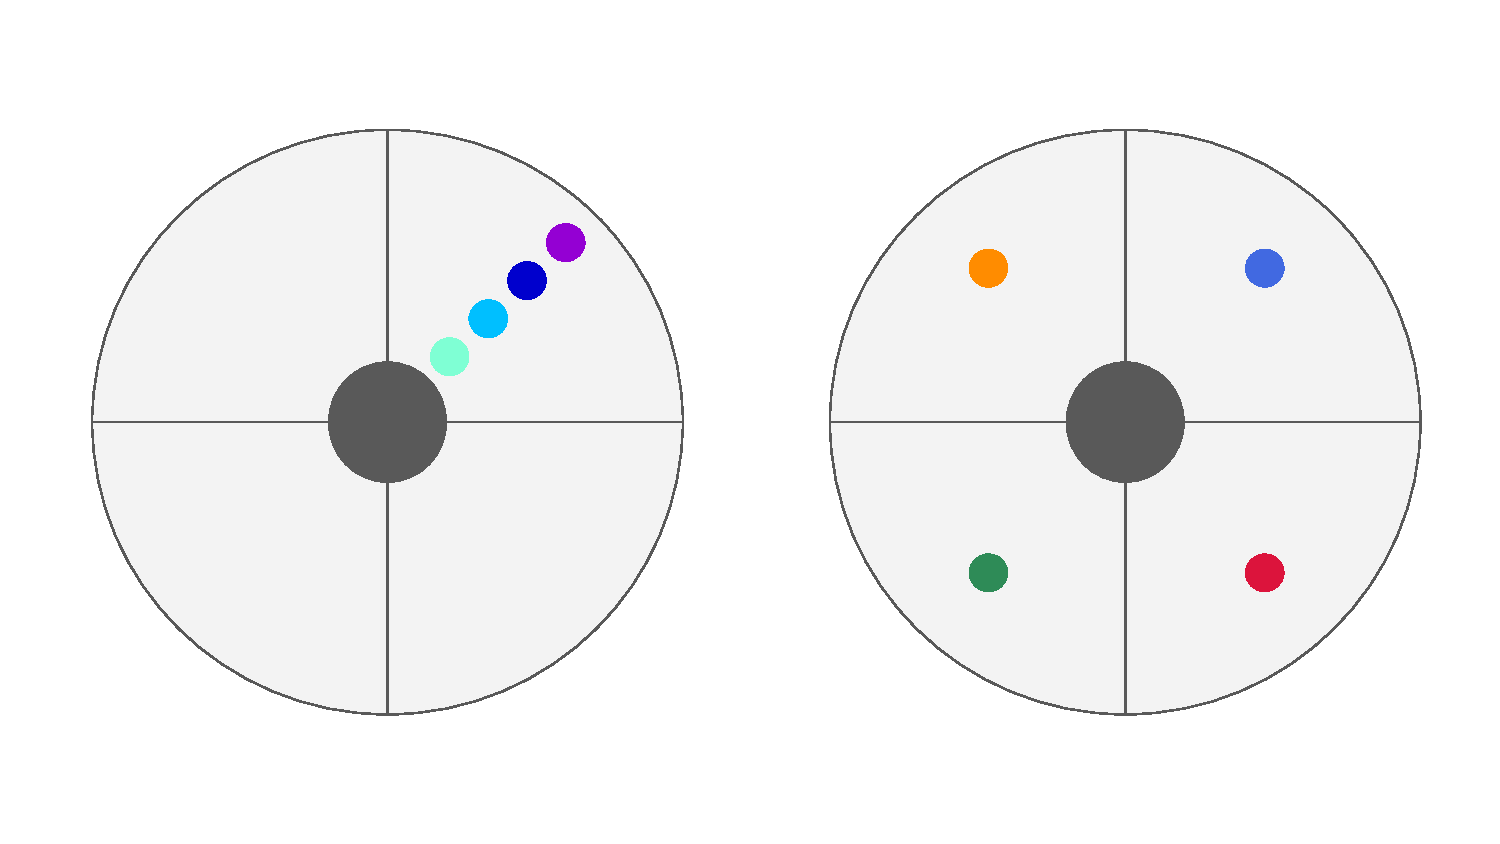
\includegraphics[width=\columnwidth]{fig/8_mirror_positions.pdf}
\caption{Left: Schematic of the 4 different radial relative positions on the primary mirror of the \SD telescope. Right: Schematic of the 4 different quadrant relative positions on the primary mirror of the \SD telescope.}
\label{fig:8_mirror_positions}
\end{figure}

\begin{figure}
    \centering
    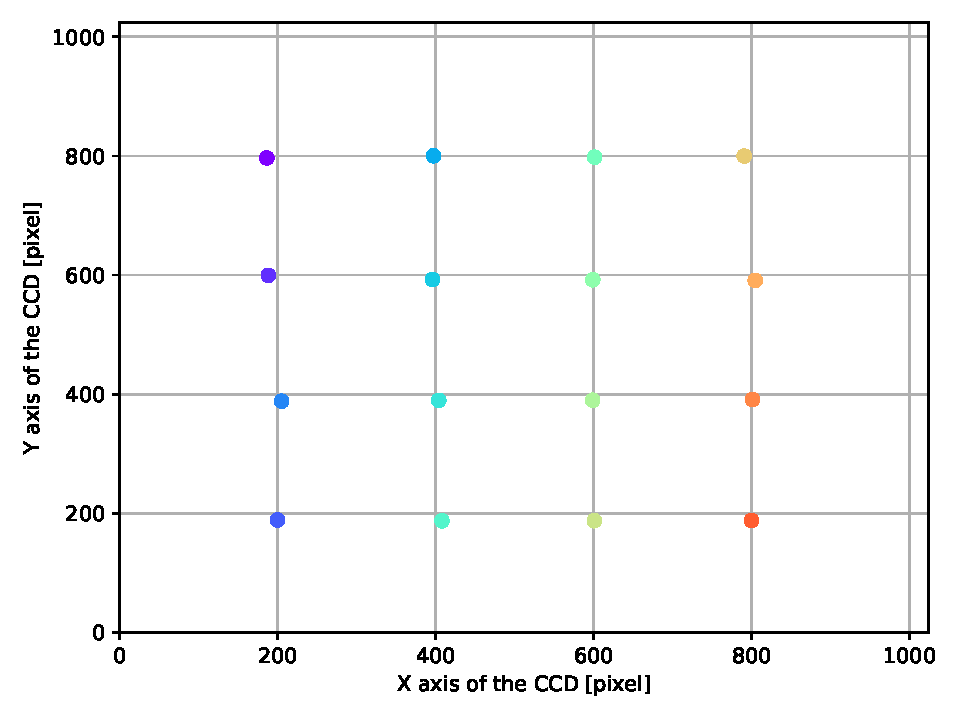
\includegraphics[width=\columnwidth]{fig/ccd_grid_colors.pdf}
    \caption{Schematic of the (4x4) grid positions on the \SD CCD focal plane.}
    \label{fig:ccd_grid}
\end{figure}

\newpage

\section{CBP response calibration with a solar cell}
\label{sec:rcbp}

\subsection{Optics setup}

The CBP optics have two degrees of freedom that must be adjusted
before determining its transmission: (1) the focuser distance, which
needs to be tuned so that the pinhole is at the focal plane of the
telescope and produces a collimated beam; and (2) the size of the iris
diaphragm, which needs to be adjusted so that no light misses the CBP
secondary mirror.

To adjust the focuser distance, we re-imaged the CBP pinhole in the
StarDICE camera using the StarDICE telescope set up for infinity
focus. We then adjusted the CBP focus to minimize the size of the
image in the camera and tightened the locking screws. However, since
this procedure was conducted before the first stellar light of the
StarDICE telescope, we had to use a theoretical value for its focal
plane position. As a result, we estimate that the collimation of the
CBP beam may be off by up to $\delta f / f = 0.002$. We did check that
the focus was reasonably stable to manual changes of the pinhole
slots.

To adjust the size of the iris diaphragm, we gradually closed it while
monitoring the flux output of the CBP until the flux started to
decrease. We then locked the diaphragm at the position immediately
preceding the flux drop. This ensured that no light was missed by the
CBP secondary mirror.

\subsubsection{Alignment of the CBP}

To measure the CBP response, we must ensure that we aim toward the solar cell. For that, we studied the signal collected in the solar cell $\Qsolarmes$ with respect to the CBP mount coordinates in azimuth and altitude. We defined the position at which we park the CBP mount when no measurement is taken at $(\mathrm{alt} = \SI{0}{\degree}, \mathrm{az} = \SI{0}{\degree})$, and the coordinates in the figure \ref{fig:cross_sc} are relative to this origin. With this figure, we can estimate the coordinates at which $\Qsolarmes$ is maximum, corresponding to the solar cell coordinates in the CBP mount frame of reference. We set the solar cell coordinates at $(\mathrm{alt} = \SI{6}{\degree}, \mathrm{az} = \SI{10}{\degree})$. These coordinates correspond to the point aimed by the CBP optics for any further solar cell analysis in this paper.

\begin{figure}[h]
    \centering
    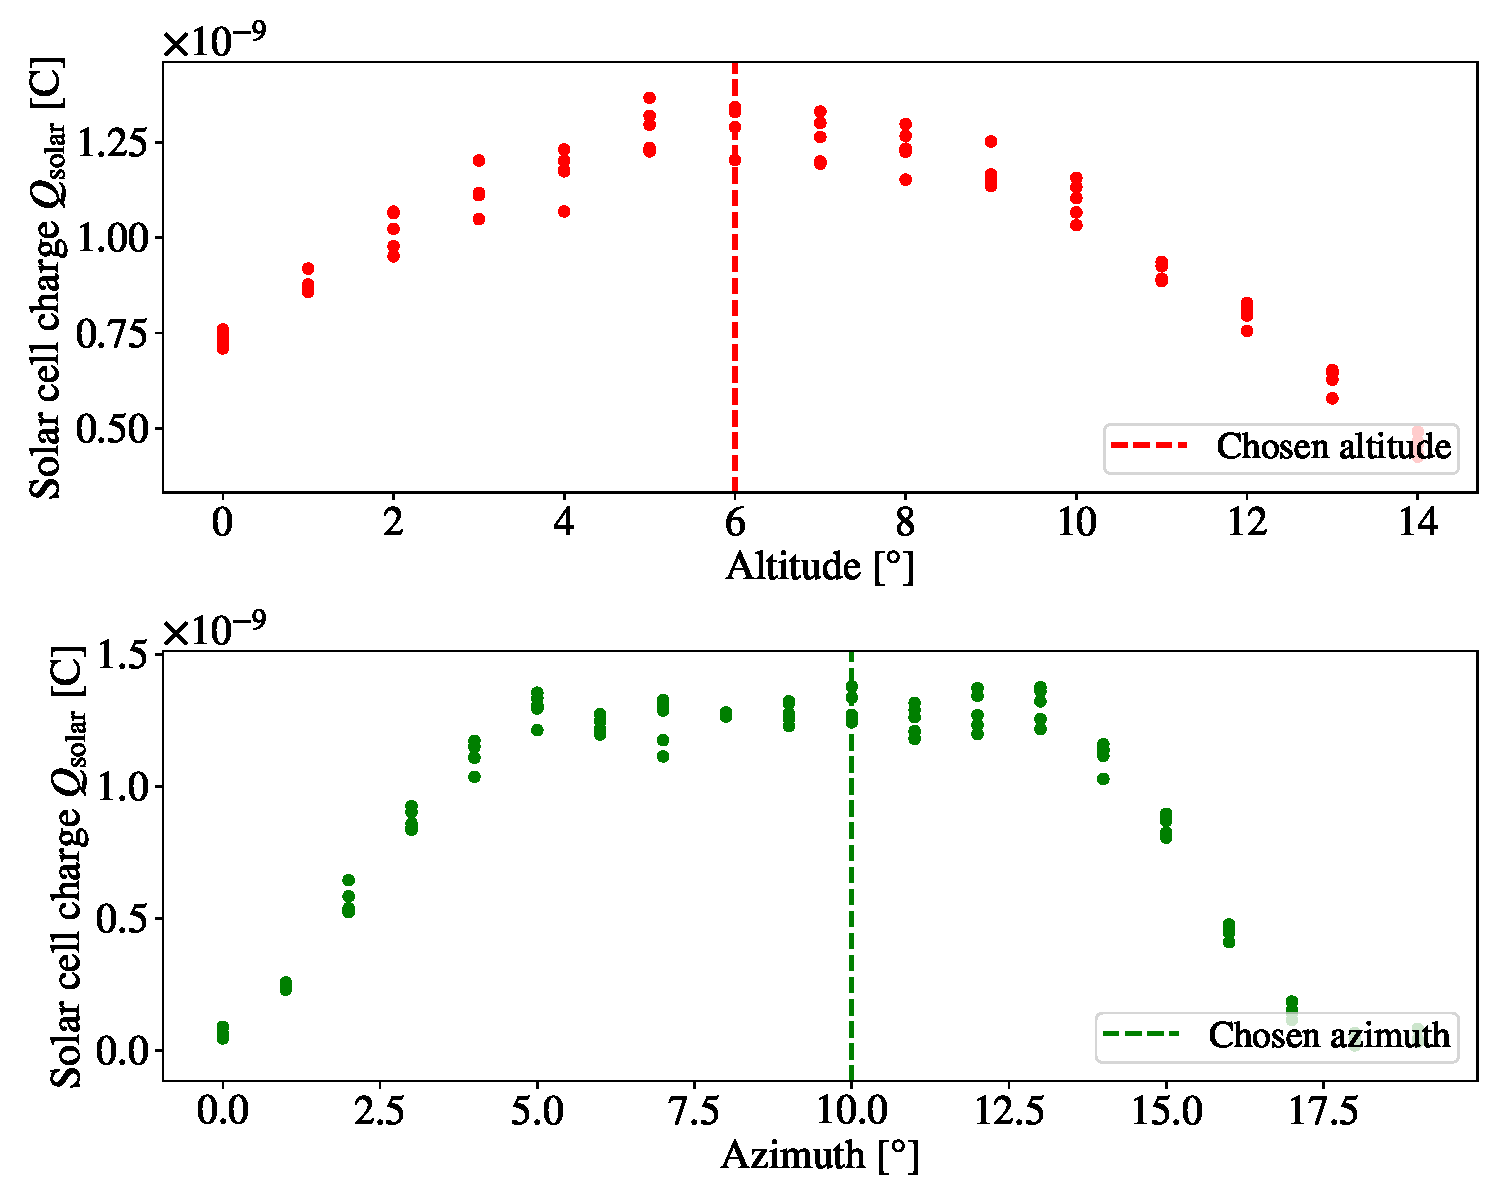
\includegraphics[width=\columnwidth]{fig/cross_solarcell.pdf}
    \caption{Evolution of the solar cell charge $\Qsolarmes$ with respect to the CBP mount coordinates. Left: evolution with respect to the altitude coordinate. Right: evolution with respect to the azimuth coordinate.}
    \label{fig:cross_sc}
    %/stardice/analysis/cbp_paper/golden_sample_analysis/dr2/cross_solarcell.ipynb
\end{figure}


\subsection{Description of the CBP data set}
\label{sec:cbp_datadesc}

\begin{figure*}[!h]
\centering
%cbp_paper_plots
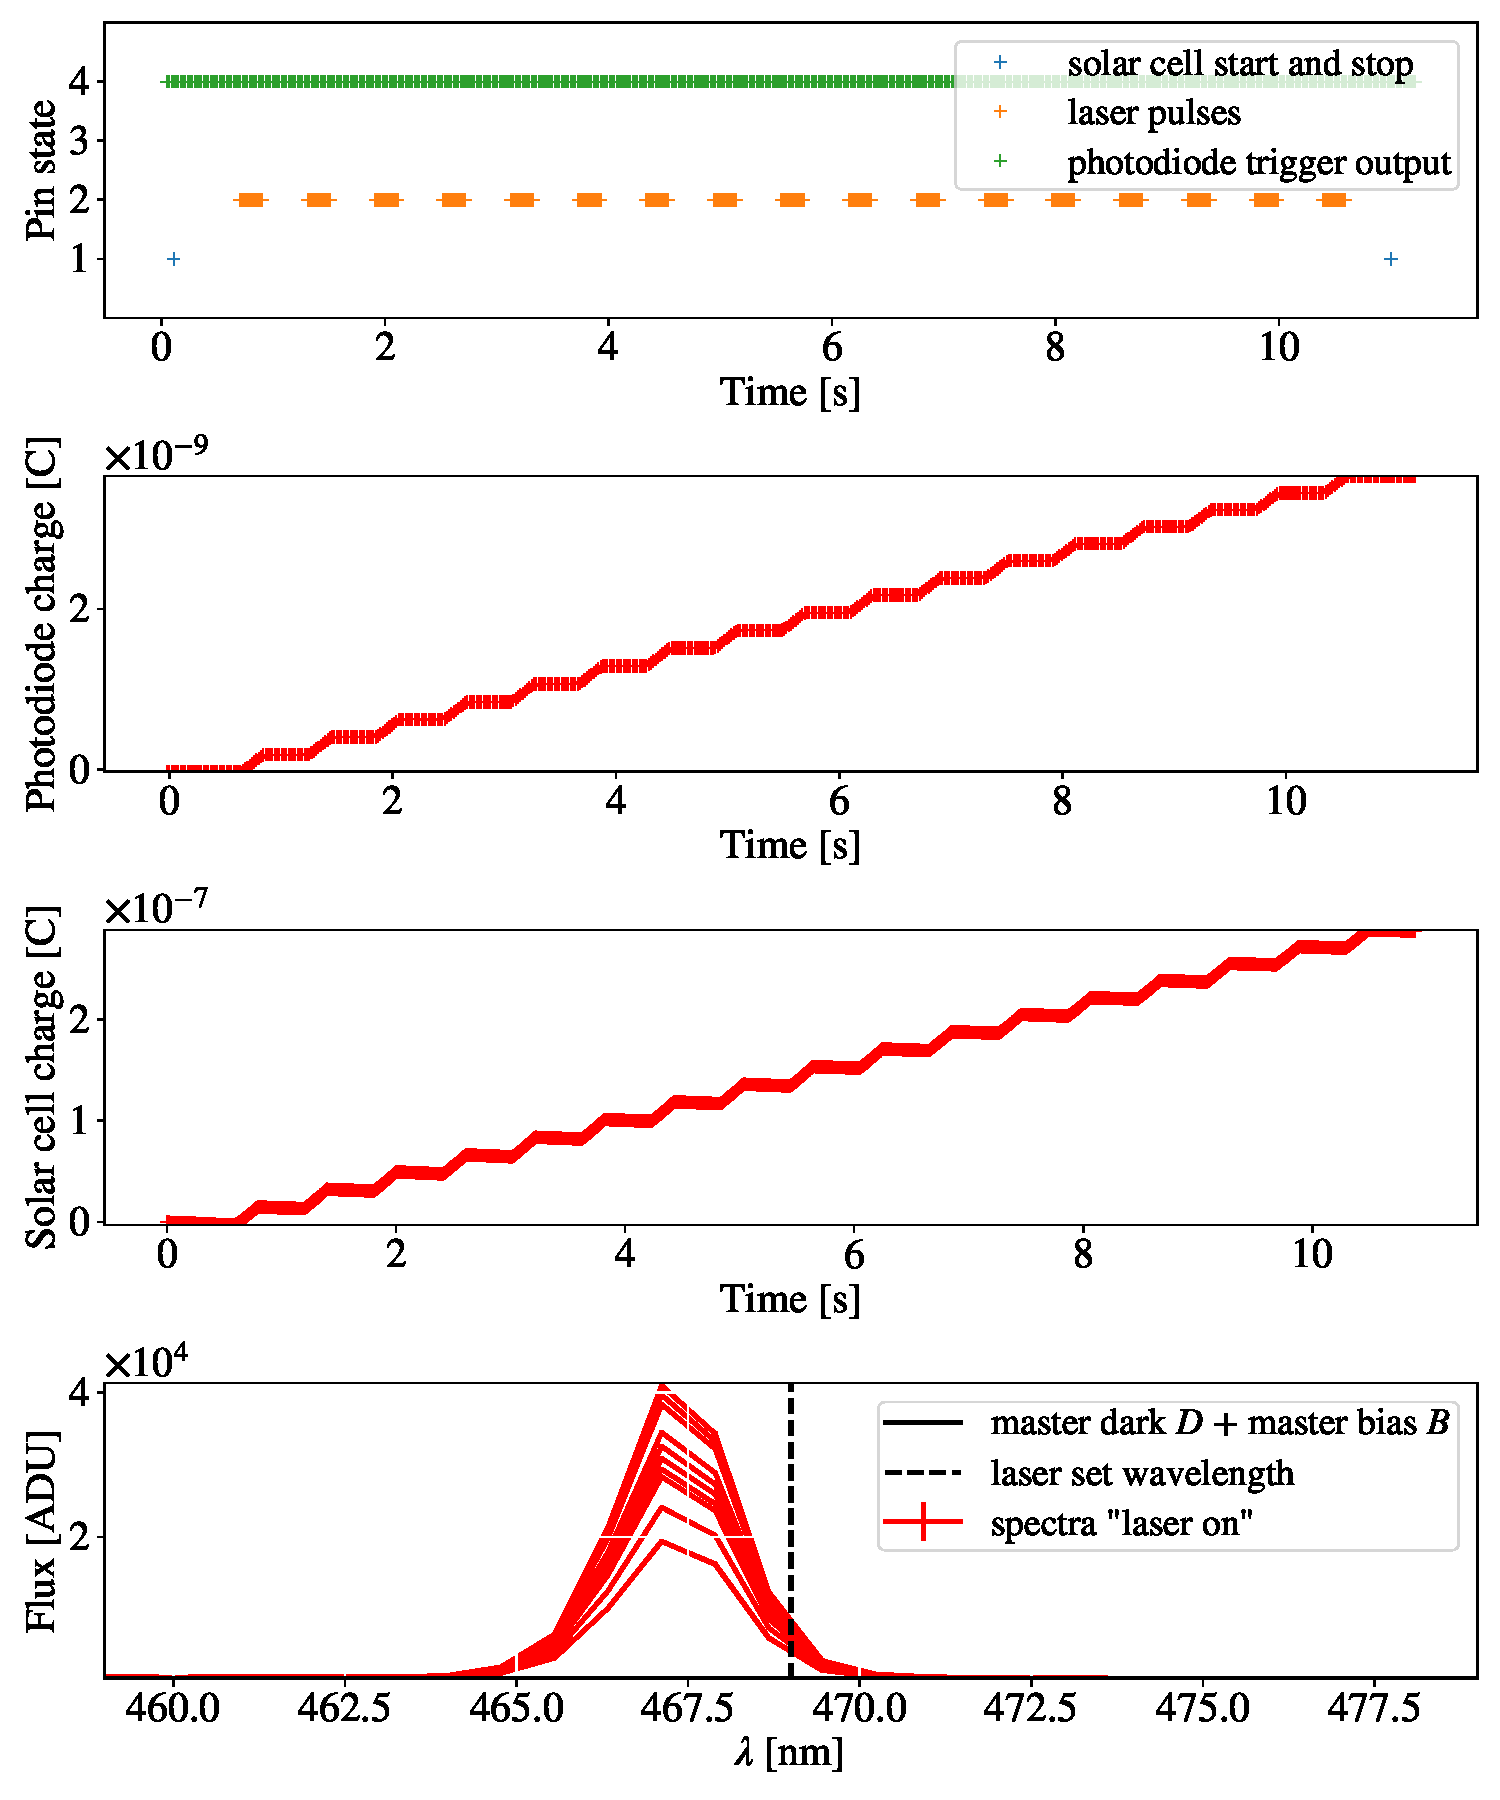
\includegraphics[width=\columnwidth]{sc_dataset_469}
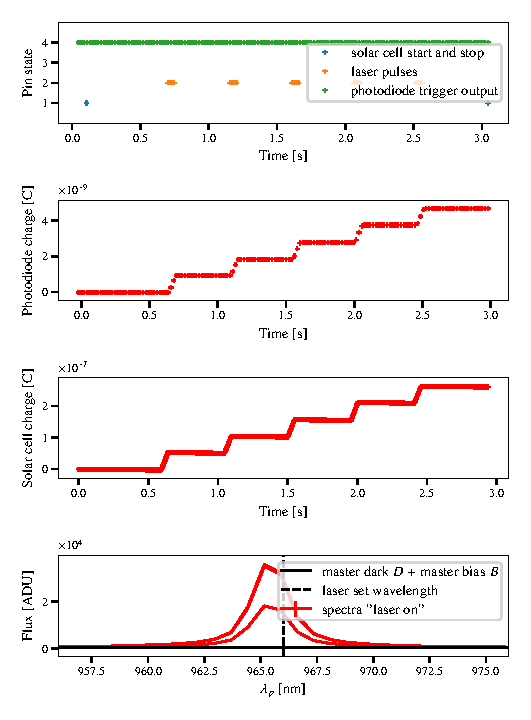
\includegraphics[width=\columnwidth]{sc_dataset_966}
\caption{Data set examples when targeting the solar cell. From top to bottom: typical data sets for digital analyser (pin state 4 is the Keithley output, pin state 2 the laser trigger output, pin state 1 the Keysight start and end time acquisition time stamps), charges in the photodiode, charges in the solar cell, flux in the spectrograph. Left: typical data set at \SI{469}{\nm}. Right: typical data set at \SI{966}{\nm}.}\label{fig:sc_dataset_examples}
\end{figure*}

A typical dataset to measure the CBP response is the emission of laser bursts in the solar cell at a given wavelength. Charges in the photodiode and solar cell are recorded jointly, along with the flux in the spectrograph and the time stamps in the digital analyser (see examples in Figure~\ref{fig:sc_dataset_examples}).

The laser emits pulses at a fixed rate of \SI{1}{\kilo\hertz}, with a power that highly depends on the wavelength. To ensure that all instruments work in their linear regime, without saturations, and limit the impact of dark current fluctuations, we decided to shoot light in the solar cell in bursts of pulses, separated by dark times at least as long as the burst length. The number of pulses per burst at each wavelength was selected to minimize the change in total flux per burst collected by the photodiode over the full wavelength range, which is the common instrument between the CBP and \SD response measurements and the one receiving the maximum power in the system (Figure~\ref{fig:npulses}). With the \SI{5}{\mm} pinhole with the largest laser power mode the solar cell accumulates around \SI{4}{\nano\coulomb} in a burst. In order to keep the $1/f$ noise of the solar cell instrumental chain under reasonable bounds, we limited the maximum length of a burst to \SI{200}{\ms}. The CBP system's linearity is checked by varying the laser power in Section~\ref{sec:sc_linearity}.  The required total flux in the photodiode was then adjusted by accumulating several bursts measured independently by the solar cell.

During a solar cell measurement run, the laser wavelengths range between \SI{350}{\nano\meter} and \SI{1100}{\nano\meter} included with steps of \SI{1}{\nm}, but are randomly chosen to avoid that long-range $ 1/f$ mode in the solar cell dark current correlates neighboured data points of the CBP response. Several runs were accumulated to enhance the signal-to-noise ratio. In particular, five runs (dataset No.~4 from Table~\ref{tab:schedule}) were recorded just before the \SD telescope measurement (dataset No.~5), and five new runs (dataset No.~6) were launched just after.

Runs with different settings have been conducted to estimate systematic uncertainties, we varied the laser global power (QSW) to assess the linearity of the instrumental light (dataset No.~4 and 6). Additionnaly, we checked the ambient light additive contamination (dataset No.~10) and varied the solar cell distance to estimate the output CBP scattered light (dataset No.~11).

%cbp_paper_plots.py
\begin{figure}[!h]
\centering
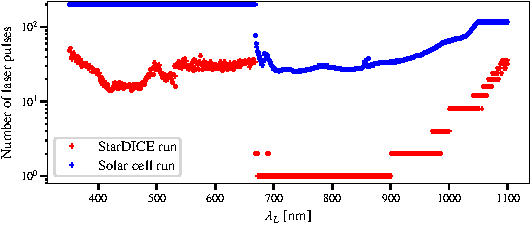
\includegraphics[width=\columnwidth]{npulses}
\caption{Number of laser pulses per burst used for solar cell and StarDICE runs.}\label{fig:npulses}
\end{figure}

\subsection{Spectrograph data reduction}
\label{sec:spectro_reduction}

In our analysis, the spectrograph is used to monitor the laser wavelength, and the contamination by laser stray light. The main components of the contamination are a \SI{1064}{\nm} line from the Yagg laser pump and a \SI{532}{\nm} half harmonic. Here, we detail the wavelength and flux calibration procedures for this instrument.


\subsubsection{Spectrograph error model estimation}

The spectrograph was characterised by taking a series of dark exposures with four different exposure times (the same used in the CBP response measurement) to evaluate its gain and readout noise. The goal is to build an error model for the spectrograph.

For each exposure time, a master dark is constructed, averaging all the spectra. Then, for each spectrograph pixel, we fitted a line through the master dark values as a function of the exposure times. The intercept gave the sensor bias value for each pixel, and a master bias $B(\lambda_p)$ is assembled from the intercept values, with $\lambda_p$ the raw spectrograph wavelength value before any calibration associated with each sensor pixel $p$. 

The master bias was subtracted from all dark exposures. From those data, we measured the readout noise and sensor gain. Let's call $D(\lambda_p)$ the dark exposure minus the master bias value for pixel $p$. For each exposure time, the variance $\sigma_p^2$ and average $\bar{D}(\lambda_p)$ of each $D(\lambda_p)$ pixel were computed. The variance evolution with the average is well described by a second-order polynomial function, parameterised as follows:
\begin{equation}\label{eq:spectro_error_model}
\sigma^2_p =\sigma_{ro}^2 +  \bar{D}(\lambda_p)/G + \sigma_G^2 \bar{D}^2(\lambda_p)
\end{equation}
with $\sigma_{ro}$ the readout noise, $G$ the sensor gain and $\sigma_G$ a statistical noise on the gain itself. The fit of this model to data led to the following values (Figure~\ref{fig:spectro_ptc}):
\begin{align}
    & \sigma_{ro} = 1.26\ \mathrm{ADU}, \\
    & G = 25.8\ e^-/\mathrm{ADU} ,\\
    & \sigma_G = 0.7\%.
\end{align}
The first two values are compatible with the CCD specifications given by the spectrograph vendor. 

%spectrograph_dark_and_bias.py
\begin{figure}[!h]
\centering
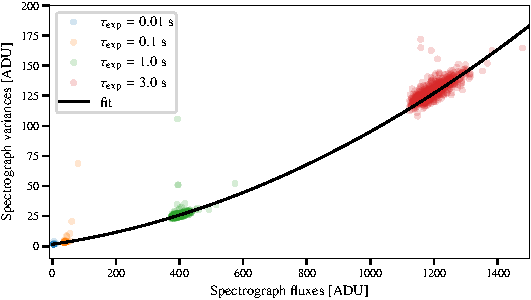
\includegraphics[width=\columnwidth]{spectro_ptc}
\caption{Spectrograph photon transfer curve to estimate gain and read-out noise. Pixel variance from dark spectra is represented versus their averages for four different exposure times $\tau_{\mathrm{exp}}$.}\label{fig:spectro_ptc}
\end{figure}


\subsubsection{Spectrograph data extraction}


The spectrograph exposure times were adjusted to avoid the saturation level for all wavelengths. However, the sampling rate was not tunable, and time stamps were unavailable. So we took as many spectra $N(\lambda_p)$ as possible during an acquisition and then analysed them. Some contained laser light, and others were darks. We assumed a spectrum is dark if there are no spectrograph pixels above its median plus a threshold in the region around the laser wavelength. This algorithm works for most spectra except for very weak laser lines that come too close to a hot pixel, which happens very rarely.

After sorting the spectra in two categories "laser on" and "laser off", we subtract the master bias $B(\lambda_p)$ and compute a master dark spectrum $D(\lambda_p)$, taking the median of all the "laser off" spectra (see Equation~\ref{eq:master_dark_spectro}). This master dark is subtracted from all spectra, which removes the spectrograph baseline and hot pixels. The spectra containing laser lines are stacked to increase the signal-to-noise ratio. We call $S(\lambda_p)$ the stacked spectrum after bias and dark subtraction:
\begin{align}
\label{eq:master_dark_spectro}
D(\lambda_p) & = \sum_{i \in \left\lbrace \text{laser off}\right\rbrace}\left( N_i(\lambda_p) - B(\lambda_p)\right), \\
    S(\lambda_p) & = \sum_{i \in \left\lbrace \text{laser on}\right\rbrace}\left( N_i(\lambda_p) - D(\lambda_p) - B(\lambda_p)\right).
\end{align}
The spectrograph error model is applied to get the intensity uncertainties $\sigma_p$ for each spectrum $i$:
\begin{equation}\label{eq:spectro_error_model_data}
\sigma^2_{i,p} =\sigma_{ro}^2 +  (N_i(\lambda_p) - B(\lambda_p))/G + \sigma_G^2 (N_i(\lambda_p) - B(\lambda_p))^2.
\end{equation}
As the signal-to-noise in the stacked spectrum is very high, we assimilate the $S(\lambda_p)$ value to its empirical average to get $\sigma_{i,p}$. The uncertainties are propagated to the stacked spectrum $S(\lambda_p)$.

Then, to detect emission lines in $S(\lambda_p)$, we fit locally Gaussian profiles on top of a linear background. The $\lambda_g$ fit is unweighted as for the spectrograph calibration process. We searched for the laser line and lines at \SI{532}{\nm} and from two-photon conversions. Indeed, we noticed the presence of a \SI{532}{\nm} line in the regime 532 to \SI{669}{\nm} and of a weak line when the laser is set to wavelength above \SI{1064}{\nm}. If we call $\lambda_L$ the wavelength at which the laser was set, we observed the production of photons at wavelength $\lambda_{\text{comp}}$, which seems given by
\begin{equation}
 \frac{2}{\SI{1064}{\nm}} \approx \frac{1}{\lambda_L} + \frac{1}{\lambda_{\text{comp}}}
 \end{equation} 
due to the conversion of two \SI{1064}{\nm} photons into a laser photon at $\lambda_L$ and a complementary photon at $\lambda_{\text{comp}}$ that ended in the laser beam. In practice, we observed a small emission line in the spectrograph when $\lambda_L > \SI{1064}{\nm}$, nearly symmetrical of the laser line with respect to \SI{1064}{\nm}. 

An example of a stacked spectra with the detection of the laser line at \SI{643}{\nm} and the pump line at \SI{532}{\nm} is shown in Figure~\ref{fig:spectro_reduc_643}, before spectrograph wavelength calibration. The average intensity value far from the emission lines is zero, with statistical error bars compatible with the observed dispersion. Intensity uncertainties are propagated up to the line centroid wavelength. 

%cbp_paper_plots.py
\begin{figure}[!h]
\centering
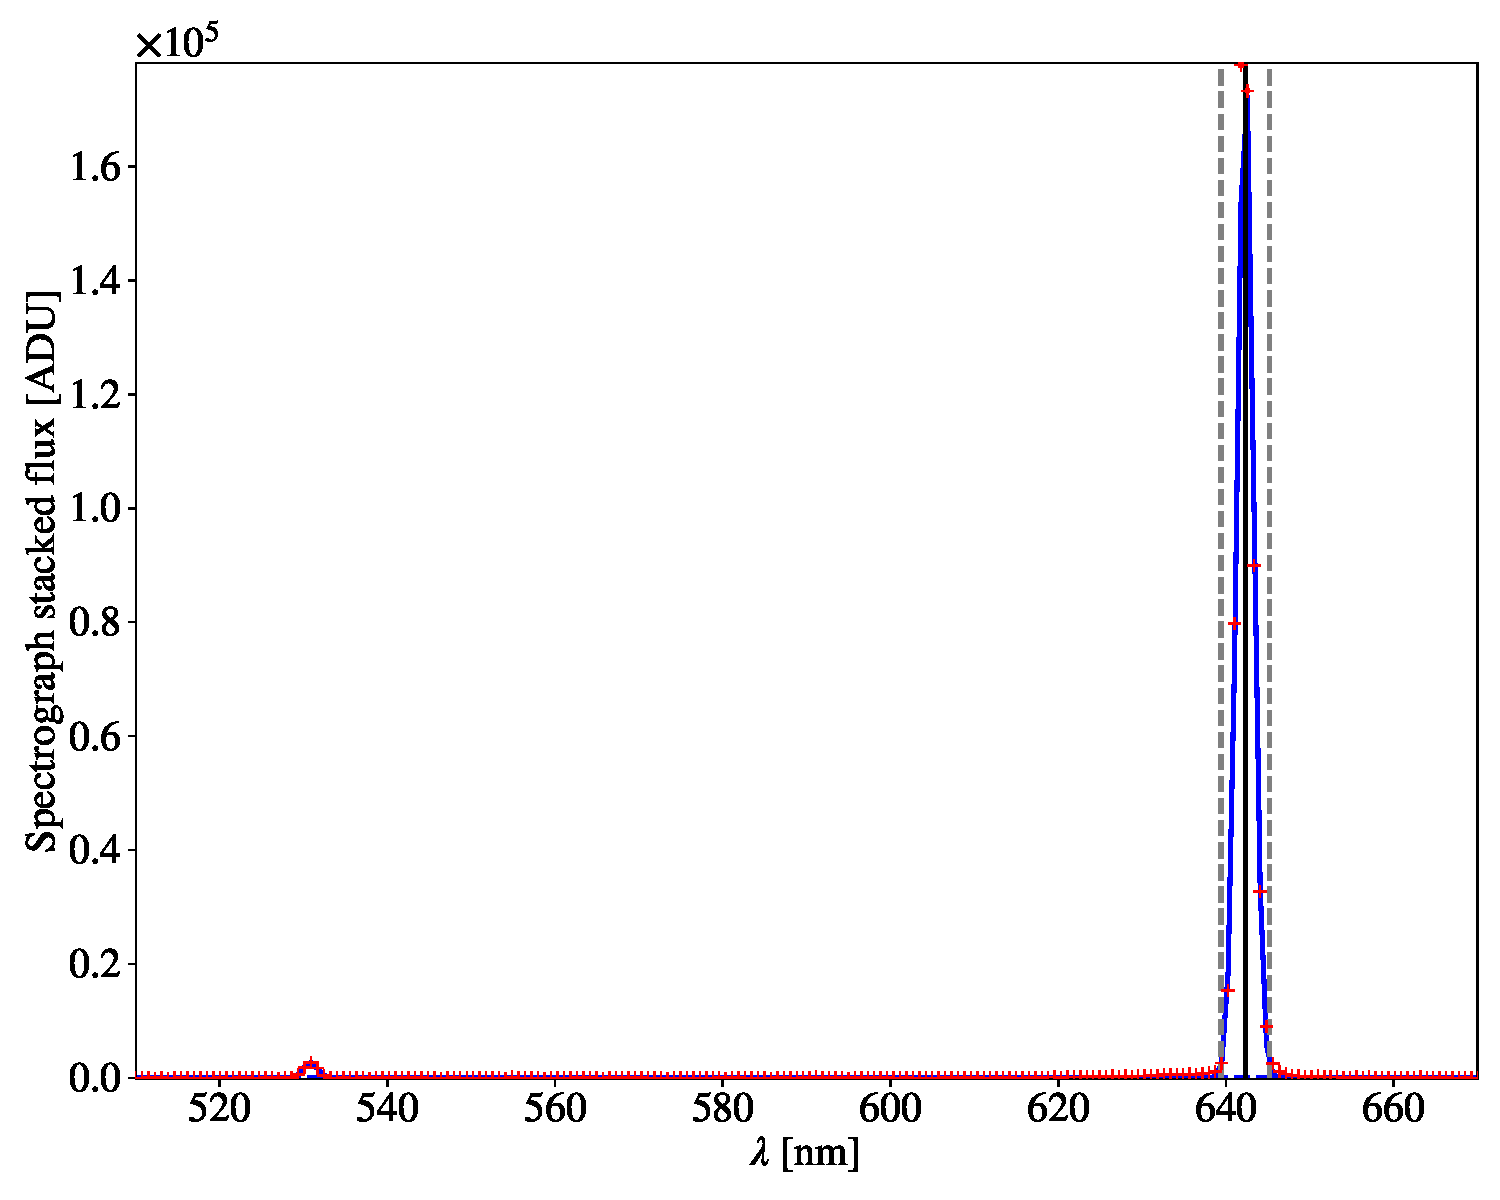
\includegraphics[width=\columnwidth]{spectro_reduc_643}
\caption{Fit of Gaussian profiles (blue lines) in the stacked spectra (red dots) for a laser line set at $\lambda_L=\SI{643}{\nm}$, with raw spectrograph wavelengths on the abscissa axis. The contamination line at \SI{532}{nm} is also visible. The black vertical line gives the fitted laser line centroid. The grey vertical lines delimit a region of $\pm 3\sigma_g$ around the centroid, where $\sigma_g$ is the fitted RMS of the Gaussian profile. The total laser flux is the sum of the pixel values in this region.}\label{fig:spectro_reduc_643}
\end{figure}


The laser line flux $\Qspectromain$, the \SI{532}{\nm} line flux $\Qspectro^{532}$ and the $\lambda_{\rm comp}$ line flux $\Qspectro^{\rm comp}$ flux are computed summing the pixels in a window of $\pm 3 \sigma_g$ where $\sigma_g$ is the RMS of the fitted Gaussian profile, after dark and bias subtraction. Associated statistical uncertainties are computed from the standard error propagation of the $\sigma_{i,p}$ values. These fluxes are used to correct solar cell and photodiode charges as well as the \SD photometry from the $\SI{532}{\nm}$ line contamination (see Section~\ref{sec:532_cont}).  %As the \SI{532}{\nm} line flux is always at most 1\% of the laser line flux,



\subsubsection{Wavelength calibration}

We calibrated the spectrograph according to the manufacturer's specifications before and after the main data acquisition run to measure the CBP and \SD responses. Light from a Hg-Ar lamp was injected into the integrating sphere to illuminate the spectrograph sensor. The master bias $B(\lambda_p)$ was subtracted from all spectra. The latter were stacked, and the spectrograph error model from equation~\ref{eq:spectro_error_model} was used to get a first estimate of the intensity uncertainties. The emission lines were fitted on the stacked spectrum using Gaussian profiles plus a polynomial background. Let's call $\lambda_g$ the line centroid fitted by this Gaussian profile. The fit is unweighted to avoid any dependence of $\lambda_g$ with the line flux and checked it was the case, but a statistical uncertainty $\sigma_\lambda^{\rm noise}$ is still estimated for $\lambda_g$ as 
\begin{equation}\label{eq:sigma_lambda_stat}
    \sigma_\lambda^{\rm noise}= \dfrac{1}{\sum_k F_k} \sqrt{\sum_p \left(\lambda_p - \lambda_g\right)^2 \sigma_p^2}
\end{equation}
with $F_k$ the flux in pixel $k$ after master bias subtraction. The sums are performed over a window of size $\pm 3 \sigma_g$ around $\lambda_g$ where $\sigma_g$ is the fitted line Gaussian profile RMS. Equation~\ref{eq:sigma_lambda_stat} corresponds to the propagation uncertainty formula for the average wavelength weighted by flux $F_p$ in a $\pm 3 \sigma_g$  window around $\lambda_g$. This allows to consider the shot noise without biasing the $\lambda_g$ fit.

To transform raw sensor wavelengths $\lambda_p$ into calibrated wavelengths $\lambda_c$, we fitted a third-order polynomial function as suggested by the manufacturer to minimise the distance to Hg-Ar tabulated values $\lambda_t$. This was done by minimizing the following function: 
\begin{equation}
    \chi_\lambda^2(a_3, a_2, a_1, a_0) = \sum_{\text{lines}} \left(\lambda_t-a_3 \lambda_g^3 - a_2 \lambda_g^2-a_1 \lambda_g -a_0\right)^2
\end{equation}
over the four polynomial coefficients $a_3, a_2, a_1$ and $a_0$. The sum is performed over lines with high significance (signal-to-noise ratio above 20), and known doublet lines were excluded. The minimisation yields  the four best-fit parameters $\hat a_i$ associated with their covariance matrix. 
As the initial Gaussian fit was unweighted, the covariance matrix $\mathbf{C}_\lambda$ is then re-scaled with a global factor to get a final reduced $\chi_\lambda^2$ of one. 
Finally, detected line centroids $\lambda_g$ are transformed into calibrated wavelengths $\lambda_c$ using the third order polynomial function $c(\lambda_g)$ with the four best fit parameters:  
\begin{equation}
    \lambda_c \equiv c(\lambda_g) \equiv \hat a_3 \lambda_g^3 + \hat a_2 \lambda_g^2+\hat a_1 \lambda_g +\hat a_0
\end{equation}
and the $\sigma_\lambda^{\rm cal}$ calibration uncertainties are
\begin{equation}
    \sigma_\lambda^{\rm cal} = \left(\vec J_c^T \mathbf{C}_\lambda \vec J_c\right)^{1/2},\quad \vec J_c = \left(\lambda_g^3, \lambda_g^2, \lambda_g, 1\right).
\end{equation}

In Figure~\ref{fig:spectro_calib_syst}, we plot the residuals of the fit $c(\lambda_g)-\lambda_t$ in the upper panel, showing the agreement between the re-scaled data uncertainties and the uncertainties propagated to the third order polynomial function $c(\lambda_g)$ using $\mathbf{C}_\lambda$. In the lower panel, the spectrograph calibration systematic uncertainties $\sigma_\lambda^{\rm cal}$ are emphasised: they are lower than $\SI{0.1}{\nm}$ in the entire wavelength range, even lower than \SI{0.025}{\nm} in the visible spectrum.

% During the data acquisition campaign, we did not unplug and plug again the optical fibre going from the integrating sphere to the spectrograph. Such an action on the spectrograph side could have changed the wavelength calibration in principle, even if beforehand, we checked the fibre placement in the spectrograph was very reproducible and did not change the wavelength scale. 

%spectrograph_calibration.py
\begin{figure}[!h]
\centering
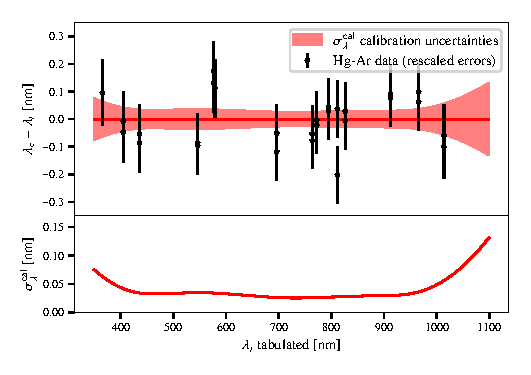
\includegraphics[width=\columnwidth]{spectrograph_calibration_syst}
\caption{Spectrograph calibration plot. Top: difference between the tabulated Hg-Ar emission line wavelengths $\lambda_t$ and the wavelengths computed using the spectrograph calibration function $c(\lambda_g)$. Data taken before and after the data acquisition campaign are superimposed. Their uncertainties were re-scaled with a common factor to get a final reduced $\chi^2$ of one. The red band represents the systematic uncertainty band from the $c(\lambda_g)$ fit on data with the uncertainty rescaling. Bottom: emphasis on the systematic uncertainties of the spectrograph calibration procedure.}\label{fig:spectro_calib_syst}
\end{figure}

We applied the third order polynomial to calibrate $\lambda_g$ into $\lambda_c$. We used the \SI{532}{\nm} line to check the quoted statistical errors $\sigma_\lambda^{\rm noise}$ on wavelength. For all data sets, we plotted the fitted line position versus time. The RMS is compatible with the quoted error bars on wavelength for lower signal-to-noise ratio data sets. But for the high signal-to-noise ratio data sets, some dispersion is unaccounted for, explained by the fact that the Gaussian profile is an incomplete model of high signal-to-noise lines. Therefore, we added a $\sigma_\lambda^{\rm PSF}=\SI{0.012}{\nm}$ statistical uncertainty due to PSF modelling on wavelength uncertainty to get a normal distribution for the residuals normalised by the full statistical uncertainties (see Figure~\ref{fig:wavelength_error_model_consistency}), the latter being
\begin{equation}
    \left(\sigma_{\lambda}^{\rm stat}\right)^2 =  \left(\sigma_{\lambda}^{\rm noise}\right)^2 +  \left(\sigma_{\lambda}^{\rm PSF}\right)^2.
\end{equation}

%cbp_paper_plots.py
\begin{figure}[!h]
\centering
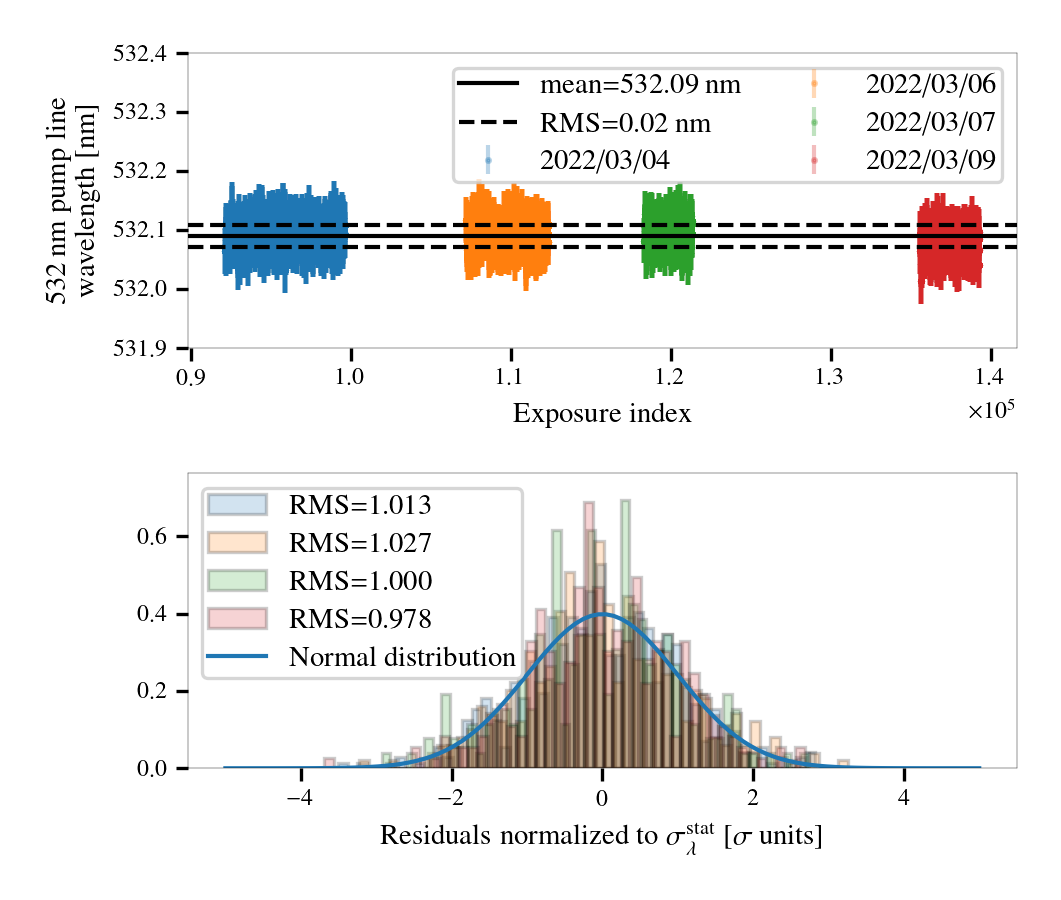
\includegraphics[width=\columnwidth]{wavelength_error_model_consistency.png}
\caption{Top: all measured \SI{532}{\nm} pump line calibrated wavelengths with respect to exposure index ($\approx\num{250000}$ data points) for the four solar cell runs. Bottom: distributions of residuals to the mean wavelength normalized by $\sigma_{\lambda}^{\rm stat}$ (colored bars) with RMS quoted in legend. A normal distribution of RMS 1 is overplotted for comparison.}\label{fig:wavelength_error_model_consistency}
\end{figure}

Finally, the wavelength uncertainty on $\lambda_c$ is
\begin{equation}
  \left(\sigma_{\lambda}\right)^2 =  \left(\sigma_{\lambda}^{\rm stat}\right)^2 +  \left(\sigma_{\lambda}^{\rm cal}\right)^2.   
\end{equation}
The composition of the final wavelength error budget is detailed in Section~\ref{sec:wavelength_syst}.


%cbp_paper_plots.py
\begin{figure}[!h]
\centering
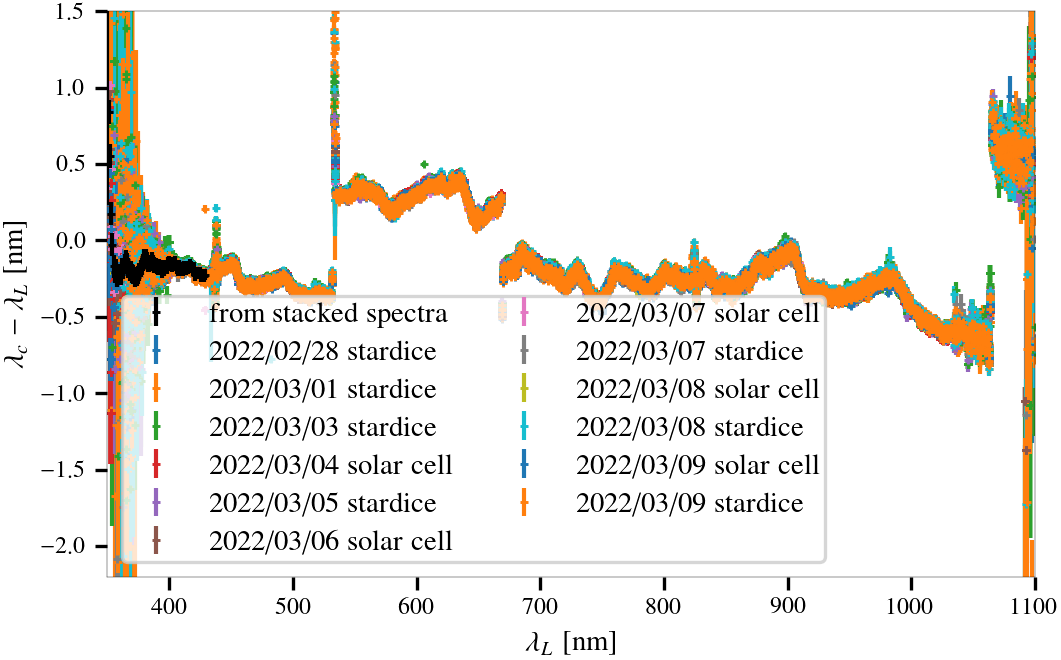
\includegraphics[width=\columnwidth]{wavelength_stability.png}
\caption{Difference between the calibrated $\lambda_c$ and requested laser wavelengths $\lambda_L$, for all the $\approx \num{350000}$ laser line wavelengths acquired during our measurement campaign.}\label{fig:wavelength_stability}
\end{figure}


The realised laser wavelength is never the one a priori asked for, as shown in Figures~\ref{fig:sc_dataset_examples} and~\ref{fig:wavelength_stability}. However, we observed remarkable repeatability of the correspondence between the set wavelength $\lambda_L$ and the realised wavelength $\lambda_c$ in Figure~\ref{fig:wavelength_stability}. This figure represents every $\approx\num{350000}$ laser bursts shot and analysed during the CBP measurement campaign. The superimposition of all measurements at each laser wavelength $\lambda_L$ exhibits good stability of the laser with time and of the $\lambda_c$ wavelength fit with line intensity. The RMS is better than \SI{0.02}{\nm} at most wavelengths, except where line determination is ambiguous: close to the contamination lines at $\SI{532}{nm}$ and $\SI{1064}{nm}$, and close to the sensor edges. Given this remarkable stability, to improve the line detection in weak laser regime (like below \SI{400}{\nm}) we averaged the obtained $\lambda_c$s for each $\lambda_L$ and decided to use this average as our final calibrated wavelength (black curve in Figure~\ref{fig:wavelength_stability}). As the bijection between $\lambda_L$ laser wavelengths and realised wavelengths $\lambda_c$ is unambiguous, in some figures of this paper, we use the set laser wavelength $\lambda_L$ for clarity. 



\subsection{Electrometer data reduction}

In one data set, we accumulated several laser bursts, and a per-burst analysis was conducted to be able to remove outliers more easily. All bursts are combined only at the end of the analysis to get the CBP and StarDICE responses.


\subsubsection{Photodiode data reduction}
\label{sec:pd_reduction}

Photodiode data are charge time series with stair-case shape. Each step is a laser burst, and the step height roughly gives the charge $\Qphotmes$ accumulated during a laser burst (see Figures~\ref{fig:sc_dataset_examples} and~\ref{fig:pd_reduc}). The length of the charge rise is the laser burst duration $\tau_b$ while flat sequences are dark times. For the photodiode, the time stamps come directly from the digital analyser clock, with a sampling at \SI{50}{\hertz}. The digital analyser clock also provides the time stamps of the laser pulses. 

For each burst, we fit straight lines in the charge sequence during the dark times before and after a laser burst, removing the closest points to the burst. We call $t_1$ and $t_2$ the time stamps of the beginning and ending of the laser burst, respectively, given by the laser trigger output itself. 
%\footnote{Technically, the laser time stamps provide the beginning of the pulse, so we add \SI{1}{\ms} to the last trigger time stamps from the laser to account for the pulse duration.}. 
The accumulated charge $\Qphotmes$ during a burst is then
\begin{equation}
q_{\rm phot}^{\rm dark}(t) = a_{\rm phot} t + b_{\rm phot}
\end{equation}
\begin{align}
\Qphotmes = \, &q_{\rm phot,2}^{\rm dark}(t_2) - q_{\rm phot,1}^{\rm dark}(t_1)\\ & - \frac{1}{2} \left[ q_{\rm phot,1}^{\rm dark}(t_2) -  q_{\rm phot,1}^{\rm dark}(t_1) + q_{\rm phot,2}^{\rm dark}(t_2) - q_{\rm phot,2}^{\rm dark}(t_1)  \right]   \notag 
\end{align}
where $q_{\rm phot,j}^{\rm dark}(t_i)$ is the line fit of the dark part $j$ ($j=1$ before the burst, $j=2$ after) evaluated at time $t_i$. The term in brackets subtract an estimation of the dark current contribution during the burst itself. After this procedure, the subtraction $q_{\rm phot,2}^{\rm dark}(t_2) - q_{\rm phot,1}^{\rm dark}(t_1)$ gives the raw height of the burst step in the charge sequence\footnote{Moreover, doing the subtraction removes systematics inaccuracy coming from the Keithley electrometer.} while the terms in brackets remove the averaged contribution of the dark current using both dark times before and after the burst. Note that we do not model anything during the burst time, as the laser power stability does not guarantee that this can be modelled with a simple mathematical function. The only model assumption is that dark sequences are modelled with straight lines.

The fit of the two parameters $a_{\rm phot}$ and $b_{\rm phot}$ of each $q_{\rm phot,j}^{\rm dark}(t)$ line models is performed via a standard $\chi^2$ minimisation, using the \texttt{curve\_fit} method from python library \texttt{scipy}. Uncertainties on the data points, equally weighted, are tuned so that the final reduced $\chi^2$ is one. As a result, we assume that the fit residuals are only due to Gaussian instrumental noise, as justified by Figure~\ref{fig:pd_reduc}. The analysis of the residuals also confirms our choice to use order 1 polynomial functions to model the dark sequences.

%cbp_paper_plots.py
\begin{figure}[!h]
\centering
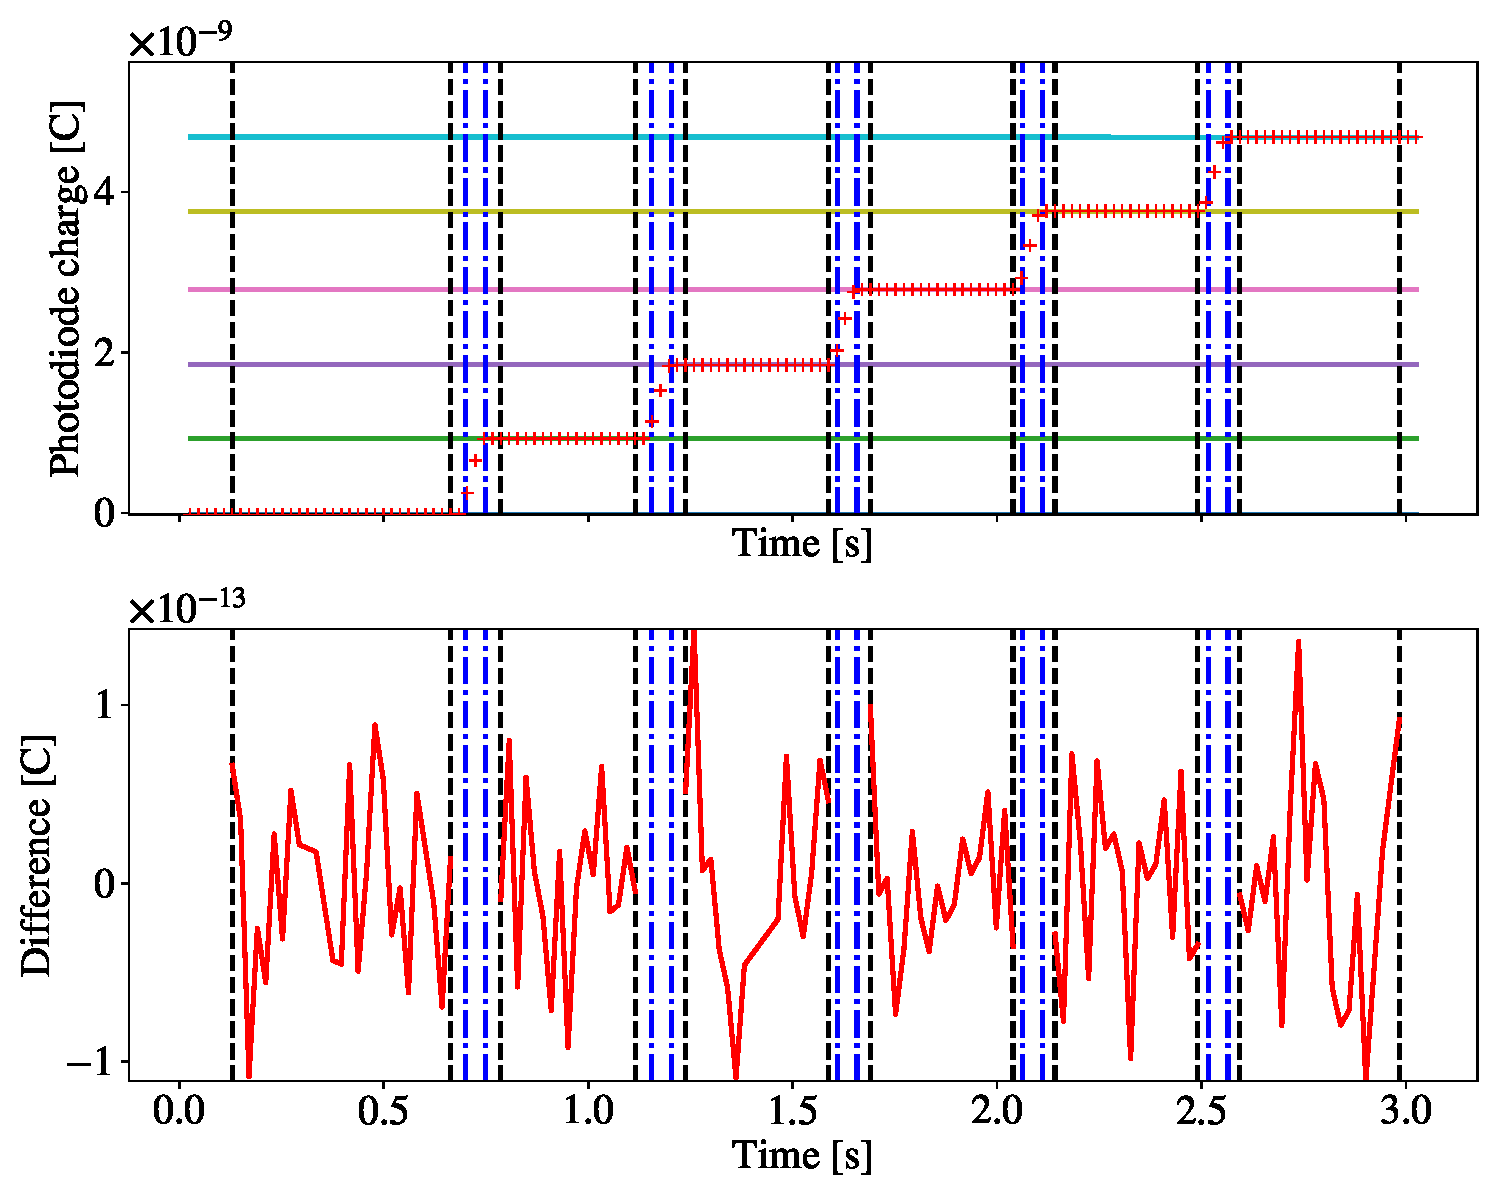
\includegraphics[width=\columnwidth]{pd_reduc_966}
\caption{Photodiode charge sequence reduction process at wavelength $\lambda_L=\SI{469}{\nm}$. Vertical blue lines indicate the laser starts and stops, while black lines flank the dark sequences. Coloured horizontal lines are fitted during dark times. The top panel shows the raw charges acquired with the photodiode, while the bottom panel shows the residuals of the linear fits during dark times.}\label{fig:pd_reduc}
\end{figure}

Covariance matrix uncertainties from all linear model parameters are then propagated to compute the statistical uncertainty $\Sphotstat$ of $\Qphotmes$ per burst. They are typically of the order of the residual RMS, around \SI{5e-5}{\nano\coulomb} (Figure~\ref{fig:pd_reduc}), more than three orders of magnitude below the typical $\Qphotmes$ values. We tested the fitting procedure on pure dark sequences and found an unbiased null measurement $\Qphot^{\rm dark}$ with a pull distribution of RMS $\;\approx 1$ whatever the burst duration $\tau_b$: computed statistical uncertainties $\Sphotstat$ nicely covers the data Gaussian noise (Figure~\ref{fig:charge_pull}).

%stardice_analysis/keithley_dark_and_bias.py
\begin{figure}[!h]
\centering
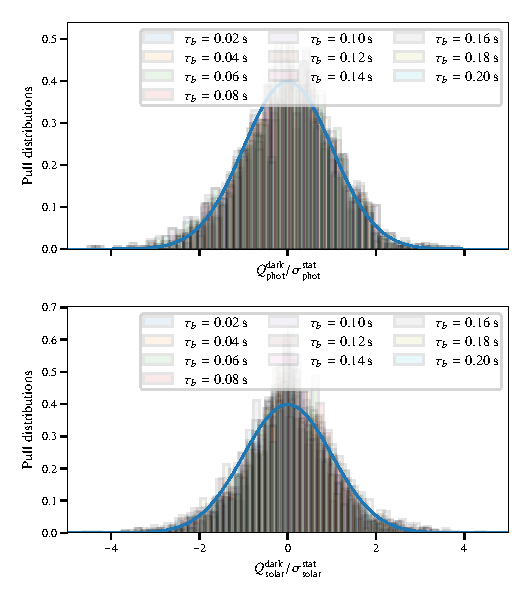
\includegraphics[width=\columnwidth]{pd_sc_stat_pull}
\caption{Top: pull distributions for photodiode charge measurements during pure dark time series $\Qphot^{\rm dark} / \Sphotstat$, with different burst durations $\tau_b$. Cyan curve represents a Gaussian distribution of mean 0 and RMS 1. Bottom: same but for the solar cell case $\Qsolar^{\rm dark} / \Ssolarstat$.}\label{fig:charge_pull}
\end{figure}



\subsubsection{Solar cell data reduction}
\label{sec:solar_reduction}

Solar cell charge time series are very similar to photodiode time series (see Figures~\ref{fig:sc_dataset_examples} and~\ref{fig:sc_reduc}). However, they are affected by two supplementary contributions as seen in the noise power spectrum: a random $1/f$ noise and power line harmonics mainly at \SI{50}{\hertz} and \SI{100}{\hertz} (Figure~\ref{fig:darkcurrentspectrum}). Timestamps come directly from the Keysight electrometer. However, as this device sends triggers at the start and end of the acquisition, the electrometer clock is re-scaled using the digital analyser. Doing so, all electrometers are synchronised via the digital analyser's internal clock.


%cbp_paper_plots.py
\begin{figure}[!h]
\centering
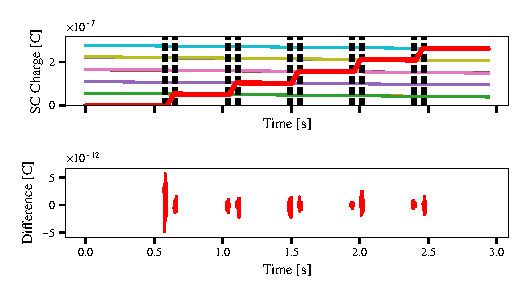
\includegraphics[width=\columnwidth]{sc_reduc_966}
\caption{Solar cell charge sequence reduction process at wavelength $\lambda_L=\SI{469}{\nm}$. Pairs of vertical black at the left and right of a burst encompass the fitted dark sequences. Coloured curves are the dark model fitted within these dark times. The top panel shows the raw charges acquired with the solar cell, while the bottom panel shows the residuals to the dark model fit during dark times only.}\label{fig:sc_reduc}
\end{figure}

As for the photodiode, we modelled the dark sequence before and after each burst. The solar cell dark model is the sum of a linear function plus two sinusoidal functions at fixed frequency \SI{50}{\hertz} and \SI{100}{\hertz}:
\begin{align}
    q_{\rm solar}^{\rm dark}(t) = a_{\rm solar}t + b_{\rm solar} & + A_{50} \sin \left( 100 \pi t + \phi_{50}\right)  \notag \\  & +  A_{100} \sin \left( 200 \pi t + \phi_{100}\right)
\end{align}
where $a_{\rm solar}, b_{\rm solar}, A_{50}, A_{100}, \phi_{50}$ and $\phi_{100}$ are free parameters fitted on data. 
Again, we call $t_1$ and $t_2$ the time stamps of the beginning and end of the laser burst, respectively, given by the laser trigger output itself.
The accumulated charge $\Qsolarmes$ during a burst is then
\begin{align}\label{eq:qsolar}
\Qsolarmes  = & q_{\rm solar,2}^{\rm dark}(t_2) - q_{\rm solar, 1}^{\rm dark}(t_1) \\  &  - \frac{1}{2} \left[q_{\rm solar,1}^{\rm dark}(t_2) - q_{\rm solar,1}^{\rm dark}(t_1) + q_{\rm solar,2}^{\rm dark}(t_2) - q_{\rm solar,2}^{\rm dark}(t_1)  \right]    \notag
\end{align}
where the indices $1$ and $2$ refer again to data before and after the burst, respectively.  Free $q_{\rm solar}^{\rm dark}(t)$ parameters were fitted, minimising a $\chi^2$ with a Newton-Raphson gradient descent. Power lines are well fitted by the model (no more periodic oscillations in the residuals) as shown in Figure~\ref{fig:sc_reduc_zoom} where $A_{50}$ was about $\SI{50}{\pico\coulomb}$.
The $1/f$ noise is not modelled in $q_{\rm solar}^{\rm dark}(t)$ as it is subdominant, but the lowest frequency modes are captured by the values of $a_{\rm solar}$ and $b_{\rm solar}$. To get a close estimate of their contributions during the burst, we fit the dark sequences only during $\tau_b/2$ around the burst to rely on their extrapolation inside the burst window (with a minimum of 12 data points to encompass at least one \SI{50}{\hertz} period). %Doing so, both linear functions are the sum of both darks containing the same $1/f$ noise power as during the laser burst and only the long-wave modes that pollute the laser burst.
Indeed, as exhibited in Figure~\ref{fig:sc_reduc_zoom}, fits of $q_{\rm solar,2}^{\rm dark}(t)$ after the first burst (orange) and of $q_{\rm solar,1}^{\rm dark}(t)$ before the second burst (green) do not superimpose because of the departure from linearity due to the long-range $1/f$ noise. So restricting the fits in two windows of size $\max(\SI{22}{\ms},\tau_b/2)$ permits to capture contaminating $1/f$ modes no longer than $\tau_b$. 

Charge value $\Qsolarmes$ is then computed for each laser burst following Equation~\ref{eq:qsolar}. Concerning estimating its statistical uncertainties $\Ssolarstat$, we add in quadrature the contributions from the parameter covariance matrix and the RMS of the residuals (to account for uncaptured $1/f$ modes). We trained the fitting procedure on pure dark data and noticed that $\Ssolarstat$ was too small to account for $\Qsolar^{\rm dark}$ null measurement dispersion. The RMS of the pull distributions was linearly dependent on the burst duration $\tau_b$, showing $\Ssolarstat$ did not capture all the long-range $1/f$ noise. Therefore, we corrected all $\Ssolarstat$ values with a multiplicative factor dependent on $\tau_b$. Doing so, we found an unbiased null measurement $\Qsolar^{\rm dark}$ with a pull distribution of RMS $\;\approx 1$ whatever the burst duration $\tau_b$ (Figure~\ref{fig:charge_pull}). 

%cbp_paper_plots.py
\begin{figure}[!h]
\centering
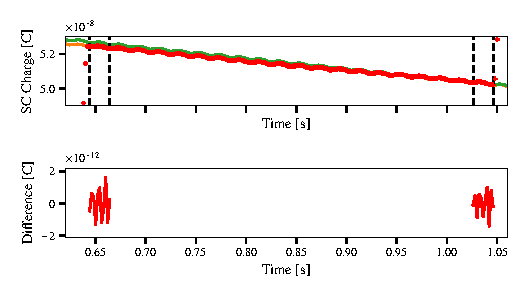
\includegraphics[width=\columnwidth]{sc_reduc_966_zoom}
\caption{Same as Figure~\ref{fig:sc_reduc} but zoomed on the second dark sequence. The orange model is fitted on dark data on the left of the plot, while the green model is fitted on dark data on the right.}\label{fig:sc_reduc_zoom}
\end{figure}


\subsection{CBP ratio of charges}

A first CBP response estimation can be computed as $r_{\rm CBP}^{\rm mes} = \Qsolarmes/\Qphotmes$ to check the statistical uncertainties and then analyse systematic uncertainties. The ratio of charges is presented in Figure~\ref{fig:cbp_charge_ratio}. Each black point is a ratio of charge measurements from one burst at one wavelength $\lambda_L$. They follow a smooth curve in $\lambda_L$. The $r_{\rm CBP}^{\rm mes}$ statistical uncertainties 
\begin{equation}
    \sigma_{\mathrm CBP}^{\rm stat} = r_{\rm CBP}^{\rm mes} \sqrt{\left(\frac{\Ssolarstat}{\Qsolarmes}\right)^2 +  \left(\frac{\Sphotstat}{\Qphotmes}\right)^2 }
\end{equation}
are higher in the blue as the laser is weaker in this regime (around $0.1\%$) than in the red (around $0.01\%$). They were estimated as the difference between all data points and a spline interpolatino, normalised by the statistical uncertainties. They follow a Gaussian distribution of mean 0 and RMS$\;\approx 1$, as expected. 

%cbp_paper_plots.py
\begin{figure}[!h]
\centering
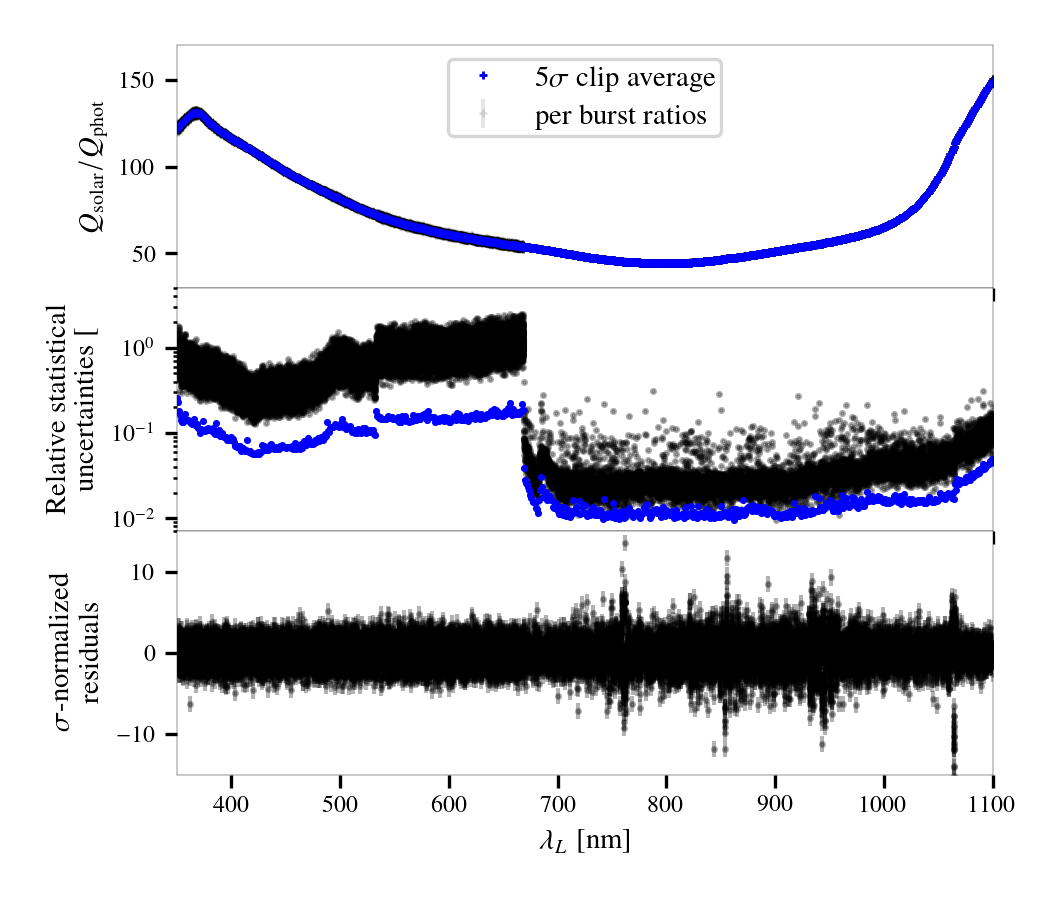
\includegraphics[width=\columnwidth]{fig/cbp_charge_ratio.png}
\caption{CBP charge ratio $\Qsolarmes/\Qphotmes$ as a function of $\lambda_L$. Top: every black point is a charge measurement ratio from one burst, the blue curve is the $5\sigma$-clipped average. Middle: relative uncertainties on $\Qsolarmes/\Qphotmes$. Bottom: pull distribution after spline subtraction.}\label{fig:cbp_charge_ratio}
\end{figure}


\subsection{Systematics}



\subsubsection{Wavelength calibration}\label{sec:wavelength_syst}


Figure~\ref{fig:wavelength_error_budget} details the total error budget from wavelength calibration for three different runs: two runs shooting at StarDICE with two pinholes and one run shooting at the solar cell. Uncertainty on wavelength $\sigma_\lambda$ is primarily dominated by wavelength calibration uncertainties in the range 400 to \SI{1080}{\nm}. Statistical uncertainty dominates around $\SI{532}{\nm}$ and close to the spectrograph sensor edges. Except in these cases, $\sigma_\lambda$ is well below $\SI{0.1}{\nano\meter}$.% which allows for precisely measuring the telescope filter band-passes better than the Angstrom level.   

%cbp_paper_plots.py
\begin{figure}[!h]
\centering
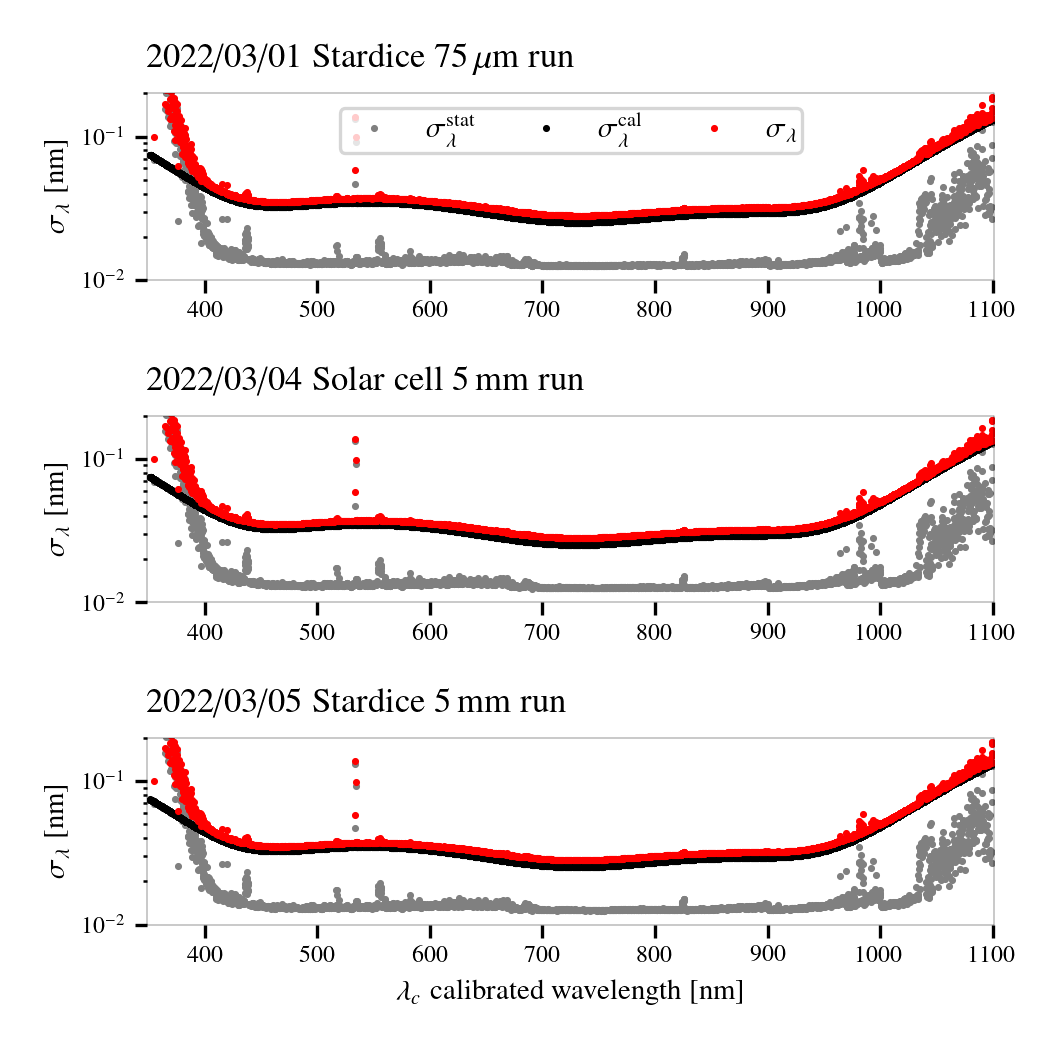
\includegraphics[width=\columnwidth]{spectrograph_error_budget.png}
\caption{Total error budget (red) of calibrated wavelengths $\lambda_c$ for three different runs (from top to bottom: StarDICE run with \SI{75}{\um} pinhole, solar cell run with \SI{5}{mm} pinhole, StarDICE run with \SI{5}{mm} pinhole) as a function of the laser set wavelength $\lambda_L$. Detection uncertainties (grey) represent PSF modelling uncertainties and Gaussian fit uncertainties, while calibration uncertainties (black) come from the Hg-Ar lamp calibration procedure. }\label{fig:wavelength_error_budget}
\end{figure}

To evaluate the systematic uncertainty on the CBP response due to the wavelength calibration, we computed $r_{\rm CBP}$ at $\lambda_c+\sigma_{\lambda^{\rm cal}}$ and $\lambda_c-\sigma_{\lambda^{\rm cal}}$. The difference between both CBP responses is well below the statistical uncertainty since the CBP response varies slowly in $\lambda$ (Figure~\ref{fig:cbp_charge_ratio}) and the whole $\sigma_\lambda$ < \SI{0.1}{\nano\meter} (Figure~\ref{fig:wavelength_error_budget}). The wavelength measurement uncertainty has a systematic effect mainly in the determination of the sharp edges of the filter band-passes.

%The importance of $\sigma_\lambda$ as a systematic uncertainty lies essentially in the determination of the telescope filter band-passes and the position of their sharp edges.


\subsubsection{Ambient light}\label{sec:sc_linearity}

 %cbp_paper_plots.ipynb
\begin{figure}[h]
    \centering
    \includegraphics[width=\columnwidth]{fig/sc_dark_qswMAX.png}
    \caption{CBP charge ratio $\Qsolar^{\rm dark}/\Qphot^{\rm dark}$ as a function of $\lambda_L$: every black point is a charge measurement ratio from one burst, the blue curve is the $5\sigma$-clipped average.}
    \label{fig:sc_dark}
\end{figure}

To check contamination by ambient light, we ran a solar cell acquisition with a cap on the CBP telescope. This mimics a regular solar cell acquisition without direct light, therefore measuring in particular the laser light leaks during operation. The measurement of this indirect ambient light $\Qsolar^{\rm dark}$ constitutes a "dark" for our CBP calibration. From this specific run, we built a dark CBP response $r_{\mathrm{CBP}}^{\rm dark} = \Qsolar^{\rm dark} / \Qphot^{\rm dark}$ where $\Qsolar^{\rm dark}$ (resp. $\Qphot^{\rm dark}$) is the burst charge collected in the solar cell (resp. the photodiode). For each $\lambda_L$, burst ratios are averaged with a $5\sigma$ clipping, giving the blue curve $r_{\mathrm{CBP}}^{\rm dark}(\lambda_L)$ in Figure~\ref{fig:sc_dark}. The high dispersion below \SI{670}{\nano\meter} corresponds to the wavelength regime where the laser power is low, inducing a faint ambient light poorly measured. The dark contribution in our solar cell data is then evaluated as follows:
\begin{equation}
    \Qsolar^{\rm dark} = r_{\mathrm{CBP}}^{\rm dark}(\lambda_L) \times \Qphotmes(\lambda_L)
\end{equation}
and subtracted from all our measurements. This correction is the main contribution to instrumental non-linearity we identified. 


\subsubsection{Laser light contamination}
\label{sec:532_cont}

As described in Section~\ref{sec:cbp}, the light source used is a tunable laser using a pump laser at \SI{532}{\nano\meter}, which has different regimes. When we operated within the range [532 - 644] nm, we detected in the spectrograph a contamination light at \SI{532}{\nano\meter} for all wavelengths in this range. 

We must account for this light contamination to get the true amount of charges $\Qsolarcal$ coming from main laser line. We built a model for the \SI{532}{\nano\meter} contribution observed in the range [532 - 644] nm. The total charge measured in the solar cell $\Qsolarmes$ is the sum of the charges from the main wavelength $\lambda_L$ and the charges from contaminations, like the \SI{532}{\nm} contamination. The same applies to the total charges measured in the photodiode $\Qphotmes$ with $\Qphot$ and $\Qphot^{532}$ respectively the charges from the main laser line and the charges from the \SI{532}{\nm} contamination:
\begin{align}
%\Qsolarmes(\lambda_L) & = \Qsolar(\lambda_L) + \Qsolar^{532}(\lambda_L) + r_{\mathrm{CBP}}^{\rm dark}(\lambda_L) \times \Qphotmes(\lambda_L) \label{eq:qsolar_mes} \\
\Qphotmes(\lambda_L) & = \Qphot(\lambda_L) + \Qphot^{532}(\lambda_L) \label{eq:qphot_mes}
\end{align}

In the spectrograph, we measured two fluxes from two separated peaks: the one from the main wavelength $\Qspectromain$, and the one from the \SI{532}{\nm} contamination $\Qspectro^{532}$. As the light is homogeneous in the integrating sphere, the proportion of contamination light and laser light is the same for  both instruments. This translates into:
\begin{equation}
    \frac{\Qspectro^{532}}{\Qspectromain} \times \frac{\Espectro(\lambda_L)}{\Espectro(532)} = \frac{\Qphot^{532}}{\Qphot} \times \frac{\Ephot(\lambda_L)}{\Ephot(532)}
    \label{eq:prev_alpha}
\end{equation}
where $\Ephot(\lambda_L)$ and $\Espectro(\lambda_L)$ are the quantum efficiencies of the photodiode and the spectrograph sensor with its optical fiber, respectively. The ratio:
\begin{equation}\label{eq:eta}
\eta(\lambda) = \frac{\Espectro(\lambda)}{\Ephot(\lambda)} = \frac{\Qspectromain(\lambda)}{\Qphot(\lambda)}
\end{equation}
can be obtained either as a dimensionless quantity from the manufacturer data sheets (Figure~\ref{fig:QEs}), or directly measured in spectrograph ADU per photodiode unit (Figure~\ref{fig:QEs}). In the following, we used the spline interpolation of the measured ratio, and quote as uncertainty the RMS of the resulting residuals.

%estimate of $\eta(\lambda)$ instead of the vendor curves, with an uncertainty given by its RMS around a smooth spline curve.

We denote the level of contamination in the photodiode $\Qphot^{\lambda_L}/\Qphot^{532}$ by the ratio $\alpha(\lambda)$ that reads:
\begin{equation}
    \alpha(\lambda_L) = \frac{\Qphot^{532}(\lambda_L)}{\Qphot(\lambda_L)} = \frac{\Qspectro^{532}(\lambda_L)}{\Qspectromain(\lambda_L)} \times \frac{\Espectro(\lambda_L)\Ephot(532)}{\Ephot(\lambda_L)\Espectro(532)} 
    \label{eq:alpha}
\end{equation}

%cbp_paper_plots.py
\begin{figure}[h]
    \centering
    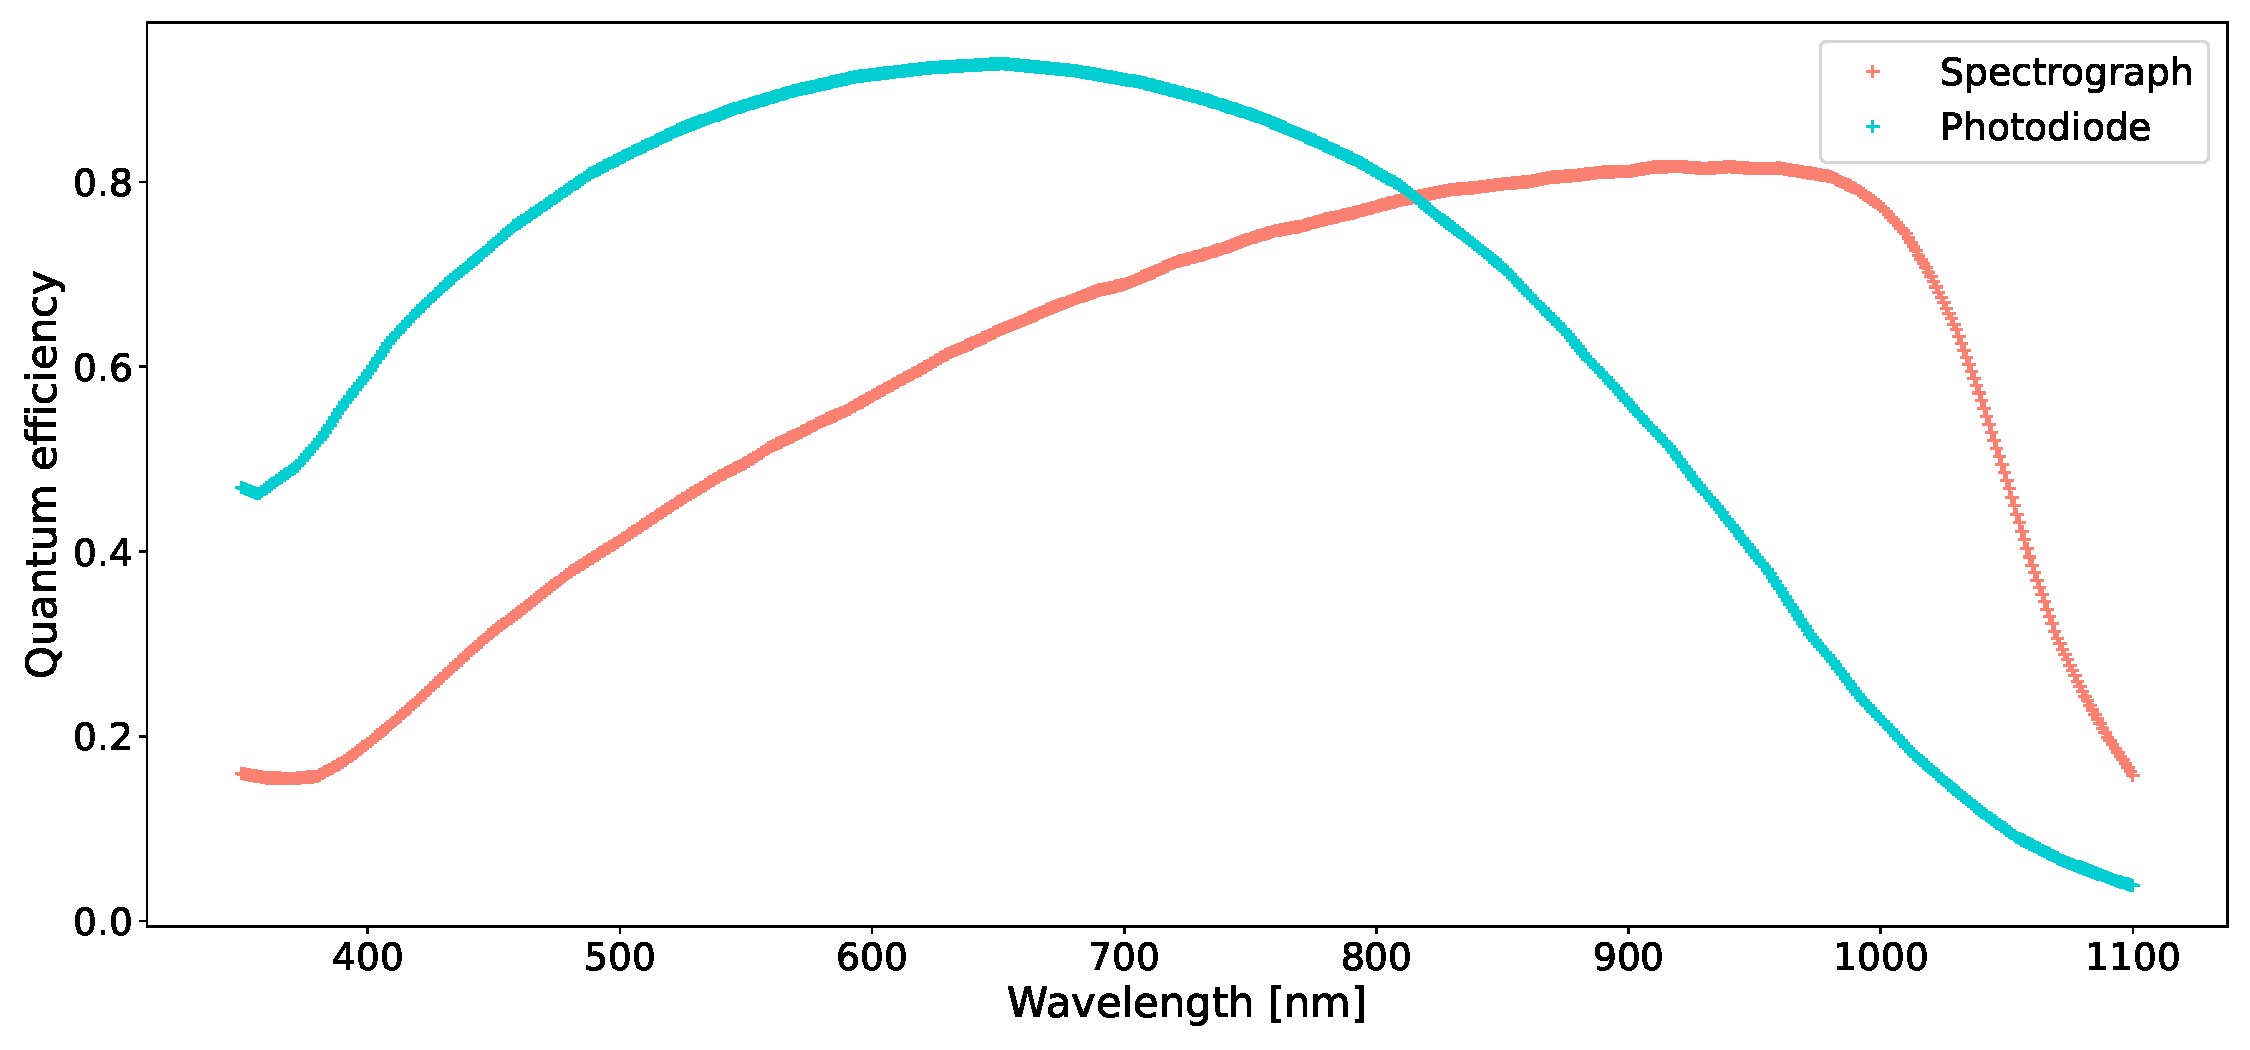
\includegraphics[width=\columnwidth]{fig/qe_phototiode_spectro.pdf}
    \caption{Quantum efficiencies of the spectrograph (red) and the photodiode (cyan), with the $\eta(\lambda)$ ratio (black).}
    \label{fig:QEs}
\end{figure}
    
We measured $\alpha(\lambda_L)$ at every wavelength using the spectrograph fluxes for the main line and the \SI{532}{nm} contaminant (Figure~\ref{fig:alpha_532}). We rejected data where $\sigma_{\lambda} > \SI{0.1}{\nm}$ in order to remove instances where the main line and the \SI{532}{nm} contaminant are poorly separated. In the 532 - \SI{540}{nm} range, where unambiguous separation between the main line and the contaminant proved infeasible, we extrapolated the $\Qspectro^{532}$ values by a linear interpolation over the full range where $\Qspectro^{532}$ was available.
The resulting $\alpha(\lambda_L)$ yield a rather flat curve between 540 and \SI{644}{\nm} with small wiggles around a global slope of $\sim 1\% $.
Uncertainties are propagated in the extrapolation range using the standard error propagation formula, taking into account the covariances between the 2 model parameters. With this $\alpha$ model, we deduced the true photodiode charges coming from the main laser line at $\lambda_L$
\begin{equation}
        \Qphotcal(\lambda_L) \equiv  \frac{\Qphotmes(\lambda_L)}{1 + \alpha(\lambda_L)} \quad\text{if}\ \lambda_L \in \left[532, 644\right]\mathrm{\,nm}\label{eq:qphot_cal532}
\end{equation}
We introduce here the notation $\Qphotcal$ as the final calibrated amount of charges detected in the photodiode per laser burst. 

Light detected by the solar cell has gone through the CBP optics, with a response $\Rcbp$.
Then, the contribution of the \SI{532}{\nano\meter} photons collected by the solar cell is computed as
\begin{equation}
\begin{aligned}
    \Qsolar^{532}(\lambda_L) & = \Rcbp(532)  \Qphot^{532}(\lambda_L) \\ 
    & = \Rcbp(532) \frac{ \alpha(\lambda_L) }{1+ \alpha(\lambda_L)} \Qphotmes(\lambda_L).
    \label{eq:qsolar_cal532}
\end{aligned}
\end{equation}
Thanks to the spectrograph data, using Equations~\ref{eq:qphot_cal532} and~\ref{eq:qsolar_cal532}, we can correct all our measurements from the \SI{532}{\nano\meter} in both the photodiode and the solar cell. The impact of this correction is illustrated in Section~\ref{sec:cbp_summary}.


\begin{figure}[h]
    \centering
    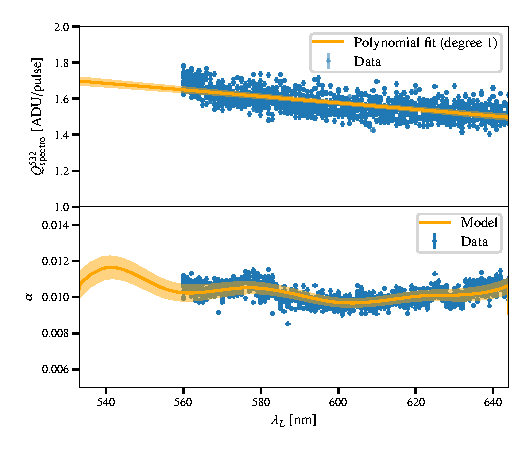
\includegraphics[width=\columnwidth]{fig/alpha_532_qswMAX.pdf}
    \caption{Top: all available data points for $\alpha$ computed from the spectrograph measurements (blue crosses) and degree 9 polynomial fit (orange) with its uncertainty (shaded orange band). Bottom: difference between data and model.}
    \label{fig:alpha_532}
    %~/stardice/analysis/cbp_paper/golden_sample_analysis/dr3/532nm_correction.ipynb
\end{figure}


We did the same correction for the complementary wavelength line $\lambda_{\rm comp}$ appearing after $\lambda_L > \SI{1064}{\nm}$. The correction coefficient $\beta$ analogue to $\alpha$ is
\begin{equation}
    \beta(\lambda_L) = \frac{\Qphot^{\lambda_{\rm comp}}(\lambda_L)}{\Qphot(\lambda_L)} = \frac{\Qspectro^{\lambda_{\rm comp}}(\lambda_L)}{\Qspectromain(\lambda_L)} \times \frac{\Espectro(\lambda_L)\Ephot\contcomp}{\Ephot(\lambda_L)\Espectro\contcomp} 
    \label{eq:beta}
\end{equation}
and is represented Figure~\ref{fig:beta}. The $\Qspectro^{\lambda_{\rm comp}}$ data points were modelled by a linear function to allow extrapolating $\beta$ in the range [1064 - 1070]\,nm. Similarly, the calibrated amount of charges in the photodiode corrected from the $\lambda_{\rm comp}$ photons is
\begin{equation}
        \Qphotcal(\lambda_L) \equiv  \frac{\Qphotmes(\lambda_L)}{1 + \beta(\lambda_L)} \quad\text{if}\ \lambda_L > \SI{1064}{\nano\meter}
        \label{eq:qphot_cal1064}
\end{equation}
and their contribution $\Qsolar^{\lambda_{\rm comp}}$ in the solar cell is given by
\begin{equation}
\begin{aligned}
    \Qsolar^{\lambda_{\rm comp}}(\lambda_L) & = \Rcbp(\lambda_{\rm comp})  \Qphot^{\lambda_{\rm comp}}(\lambda_L) \\ 
    & = \Rcbp(\lambda_{\rm comp}) \frac{ \beta(\lambda_L) }{1+ \beta(\lambda_L)} \Qphotmes(\lambda_L).
    \label{eq:qsolar_cal1064}
\end{aligned}
\end{equation}

Both corrections' impact is illustrated in Section~\ref{sec:sc_linearity} and Figure~\ref{fig:SCqswlinearity}, and Section~\ref{sec:sd_contaminations}.


\begin{figure}[h]
    \centering
    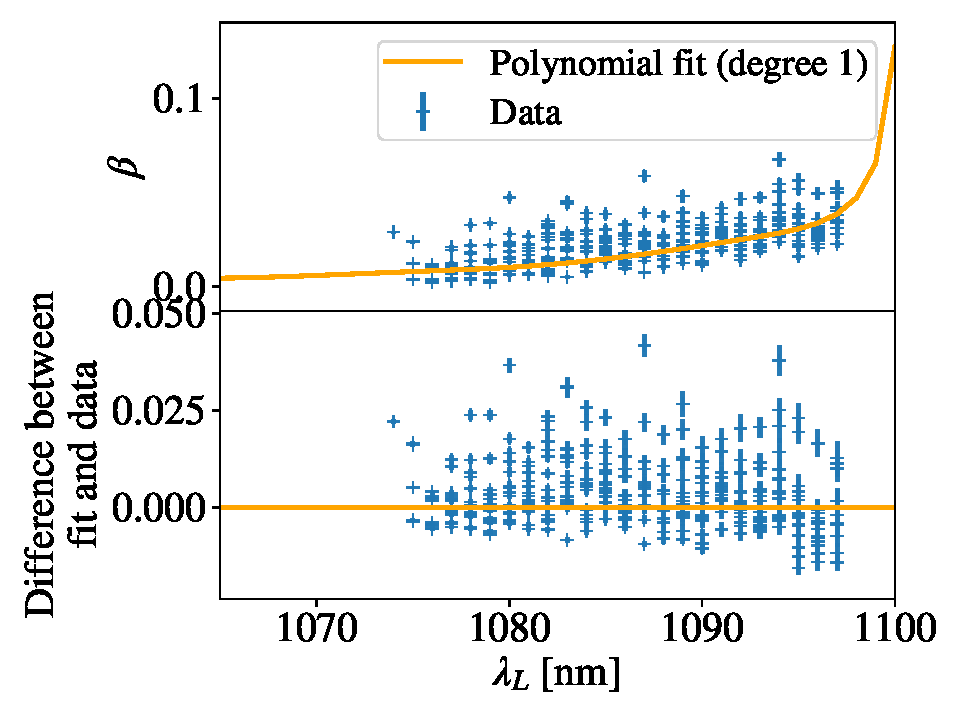
\includegraphics[width=\columnwidth]{fig/beta_532_qswMAX.pdf}
    \caption{Same as Figure~\ref{fig:alpha_532} but for $\beta$ correction coefficient.}
    \label{fig:beta}
    %~/stardice/analysis/cbp_paper/golden_sample_analysis/dr3/1064nm_correction.ipynb
\end{figure}


\subsubsection{Integrating sphere fluorescence}\label{sec:fluorescence}


\begin{figure}[h]
    \centering
    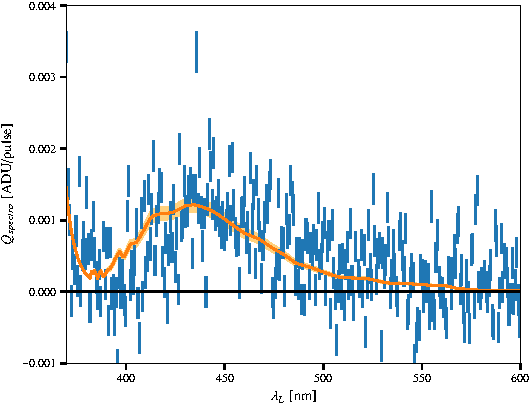
\includegraphics[width=\columnwidth]{fig/spectro_stack_fluo_model.pdf}
    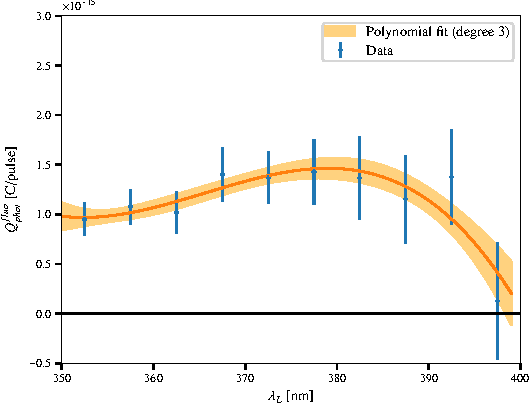
\includegraphics[width=\columnwidth]{fig/QPDfluo_model.pdf}
    \caption{Top: integrating sphere fluorescence spectrum from a stack of all solar cell run data with $\lambda_L < \SI{370}{\nano\meter}$ (blue crosses), with the best-fit model (orange line). Bottom: estimated fluorescence contribution in photodiode measured charges $\Qphot^{\rm fluo}$ as a function of wavelength (blue crosses) with a fitted third-order polynomial function (orange line).}
    \label{fig:fluo}
    %~/stardice/analysis/cbp_paper/golden_sample_analysis/dr3/1064nm_correction.ipynb
\end{figure}

Our integrating sphere appeared to be fluorescent at laser wavelengths below \SI{400}{\nano\meter}. The fluorescence of integrating spheres is studied in~\cite{shaw2007ultraviolet}. The fluorescent signal is visible in the \SD camera using the g filter or the grating but is very weak in the spectrograph. To visualise and model it, we stacked all our spectra in bins of \SI{5}{\nano\meter} in $\lambda_L$ (Figure~\ref{fig:fluo} top). The fluorescence signal spans a range of wavelength between $\approx \SI{400}{\nano\meter}$ and $\approx\SI{500}{\nano\meter}$, with an emission peak around \SI{450}{\nano\meter}. %The peak amplitude depends on the laser wavelength, as expected for a fluorescence phenomenon. 

To estimate the contamination from fluorescence photons, we fitted a fluorescence spectrum model taken from Figure~9 of \cite{shaw2007ultraviolet}, with a constant background and a Moffat profile for the laser line for each stacked spectra. The fluorescence spectrograph flux is converted into photodiode charges $\Qphot^{\mathrm{fluo}}$ using the $\eta(\lambda)$ conversion factor and normalised by the total number of laser pulses (Figure~\ref{fig:fluo} bottom)\footnote{Contrary to the \SI{532}{\nano\meter} line contamination correction, we can not normalise by the flux in the main laser line as it is often noise-dominated in un-stacked spectra when $\lambda_L < \SI{400}{\nano\meter}$.}. We observed that the fluorescence spectrum cancels at $\lambda_L \geq \SI{400}{\nano\meter}$. For every wavelength $\lambda_L < \SI{400}{\nano\meter}$, we evaluate and subtract the contribution from the fluorescence contamination in the photodiode using the $\Qphot^{\mathrm{fluo}}(\lambda_L)$ model from Figure~\ref{fig:fluo}:
\begin{equation}
        \Qphotcal(\lambda_L) \equiv  \Qphotmes(\lambda_L) - \Qphot^{\mathrm{fluo}}(\lambda_L) \quad\text{if}\ \lambda_L < \SI{400}{\nano\meter}
        \label{eq:qphot_calfluo}
\end{equation}
We perform identically for $\Qsolarmes$ multiplying by the CBP response at \SI{450}{\nano\meter}: 
\begin{equation}
\begin{aligned}
    \Qsolar^{\rm fluo}(\lambda_L) & = \Rcbp(450)  \Qphot^{\rm fluo}(\lambda_L)
    \label{eq:qsolar_calfluo}
\end{aligned}
\end{equation}

This correction's impact is illustrated later in Section~\ref{sec:sd_contaminations}.

After the fluorescence, \SI{532}{\nano\meter} and $\lambda_{\mathrm{comp}}$ corrections, we updated our $\eta(\lambda)$ estimate and iterated several times to refine the light contamination subtractions.


\subsubsection{Instrumental chain linearity check}\label{sec:sc_linearity}
For the two solar cell runs we undertook, we varied the laser output power by a factor of around 2, namely, QSW at maximum and QSW set at 298. The ratio of the two CBP charge ratios before and after dark subtraction is presented in Figure~\ref{fig:SCqswlinearity}. Basically, no corrections lead to a ~5 permil deviations of the two CBP responses with respect to wavelength. Both CBP responses agree at $\approx 0.5\,$permil for wavelengths above \SI{669}{\nano\meter} when applying dark subtraction. Then, laser contamination correction makes the two CBP responses agree in the [532, 669]\,nm range better than 0.1 permil.

To assess the value of systematic uncertainties on the CBP response due to non-linearities, we take the absolute distance of the binned ratio to unity in four different ranges of wavelengths after dark subtraction and laser contamination correction (red segments in the bottom plot of Figure~\ref{fig:SCqswlinearity}).

%cbp_paper_plots.ipynb
\begin{figure}[h]
    \centering
    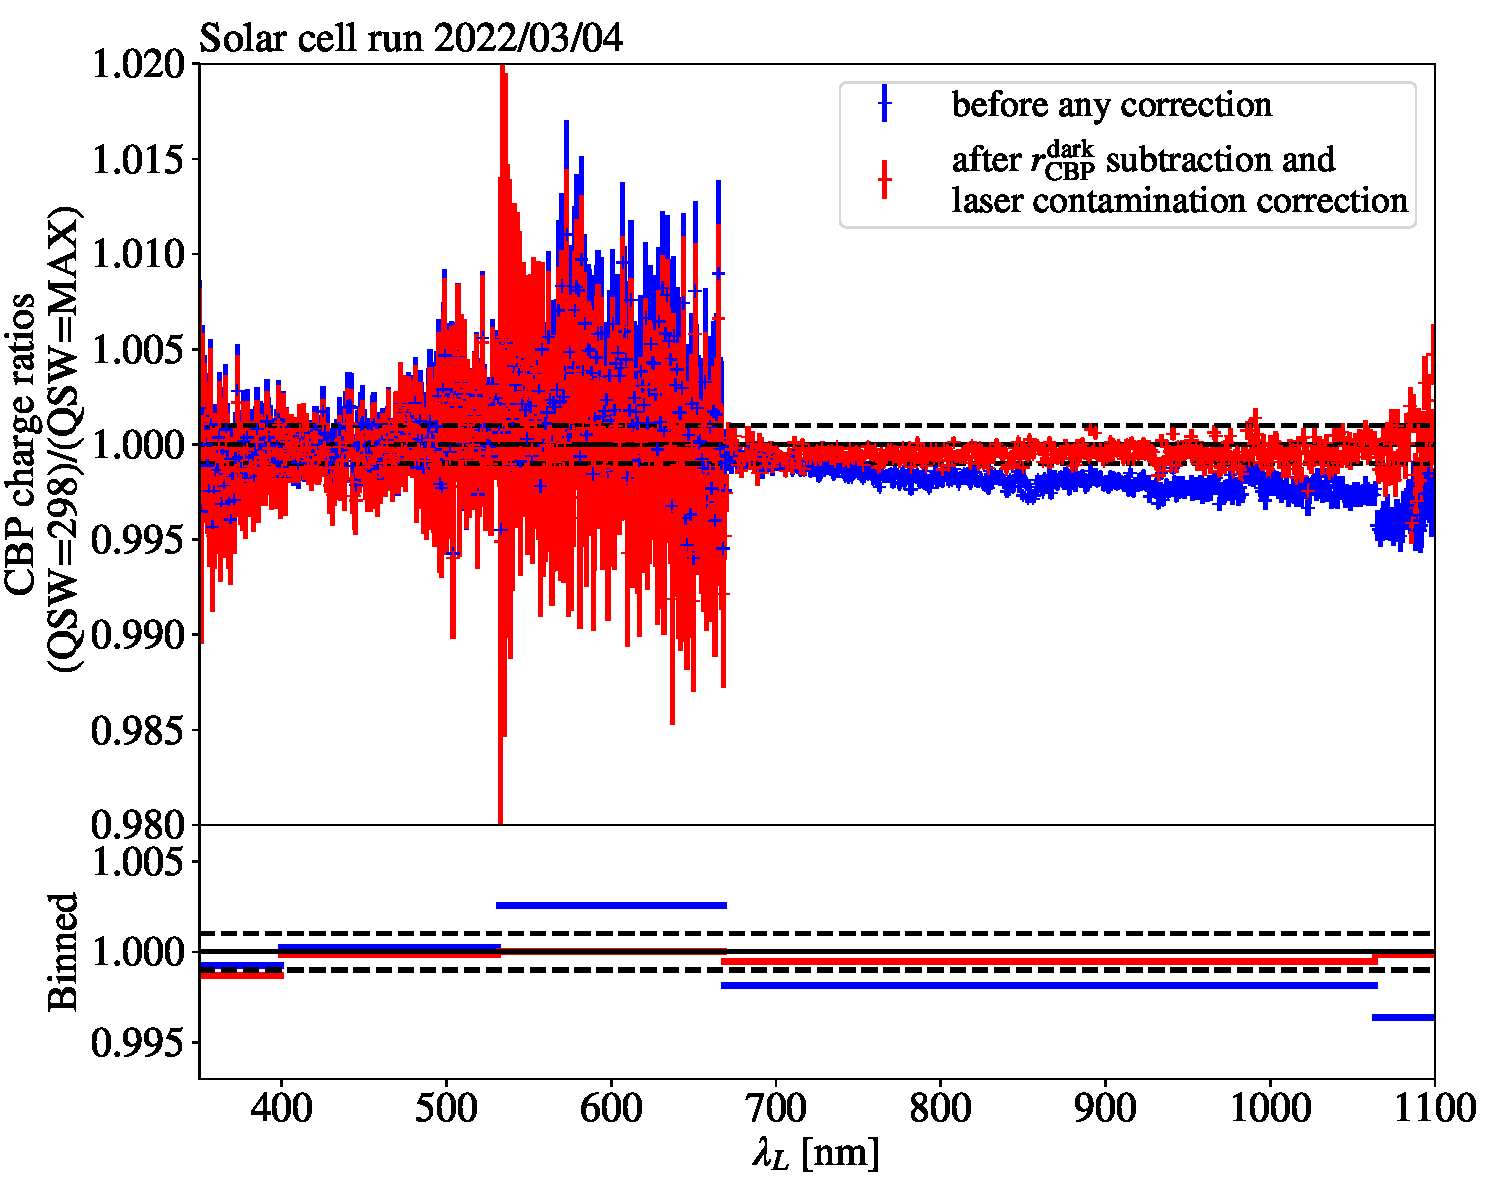
\includegraphics[width=\columnwidth]{fig/sc_qsw_ratios.pdf}
    \caption{Ratios of the CBP charge ratio for two different QSW values as a function of $\lambda_L$ coming from the 2022/03/04 solar cell run. Blue is for raw data while red is used for data corrected by dark contribution and laser contaminations. Black dashed lines encompass the permil precision region. Top: ratios for each $\lambda_L$. Bottom: binned ratio for four different wavelength ranges. A similar plot is obtained for the 2022/03/06 solar cell run.}
    \label{fig:SCqswlinearity}    
\end{figure}


\subsubsection{CBP scattered light varying the solar cell distance}

To measure the influence of scattered light in the CBP beam, we measured the CBP throughput by putting the solar cell \SI{16}{\cm} farther and compared it to the initial value. At this new position, we measured again the CBP dark from solar cell $\Qsolar^{\rm dark}$. Dark subtraction and laser contamination correction are applied. The comparison of both transmissions is presented in Figure~\ref{fig:sc_distance}. There is a decrease of the total light of about 3\textperthousand\ with a chromatic effect of about 2.5\textperthousand\ difference between \SI{350}{\nano\meter} and \SI{1100}{\nano\meter}. This constitutes the dominant systematics in the CBP throughput measurement.

%cbp_paper_plots.ipynb
\begin{figure}[h]
    \centering
    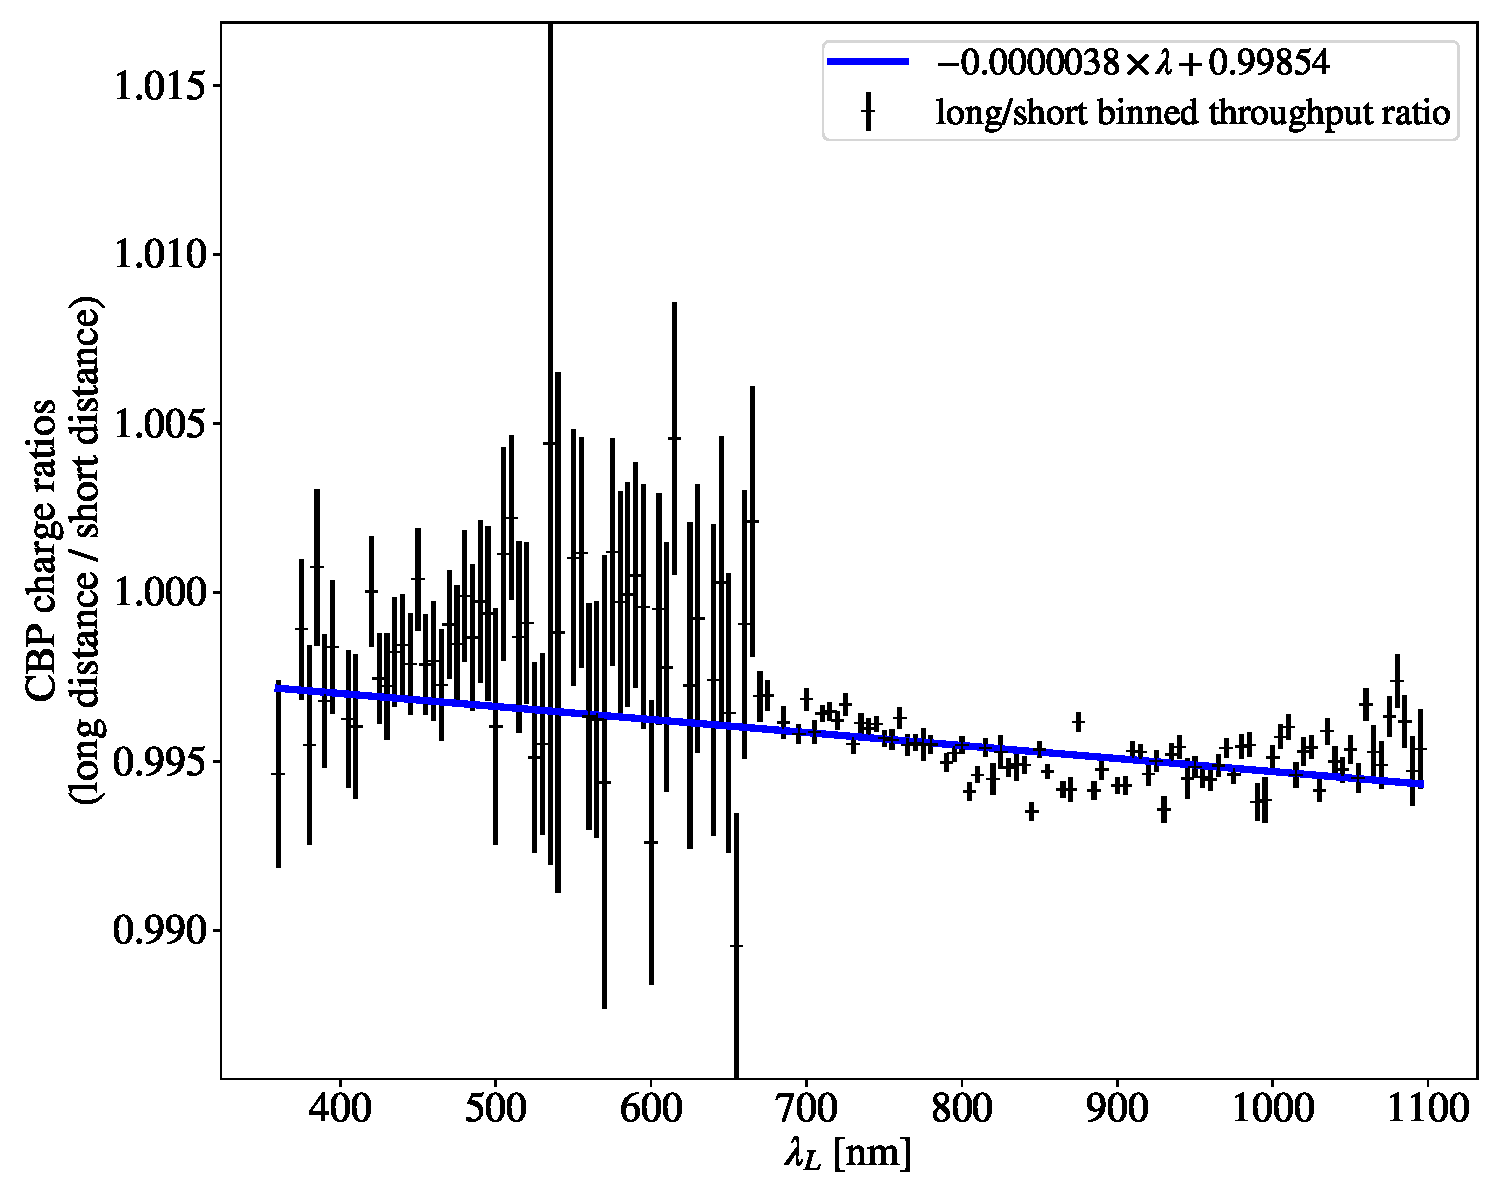
\includegraphics[width=\columnwidth]{fig/sc_distance.pdf}
    \caption{Ratios of the CBP charge ratio for two different distances to the solar cell as a function of $\lambda_L$ coming from the 2022/03/08 solar cell run. The long-distance is \SI{16}{\cm} larger than the short distance. Black points are the binned ratio for each $\lambda_L$, and the blue line is a fit whose equation is in legend.}
    \label{fig:sc_distance}
\end{figure}

\subsubsection{Repeatability}

Finally, we measured three times the value of the CBP response during our measurement campaign. For run $i$, we computed the CBP charge ratio $r_{\rm CBP}^{\mathrm{run}\ i}$, applying dark subtraction and laser contamination correction, binned in \SI{1}{\nano\meter} intervals in $\lambda_L$. Then, we computed the mean CBP response $\overline{r_{\rm CBP}}$ as the mean of the three different runs. We observed $\approx 1$\,permil differences between the three CBP charge ratios and $\overline{r_{\rm CBP}}$ (Figure~\ref{fig:SCrepeatability}), depending slightly with wavelength.


To assess the value of systematic uncertainties on the CBP response due to its stability, we take the maximum absolute distance of the binned ratio to unity in four different ranges of wavelengths (segments the farther from 1 in the bottom plot of Figure~\ref{fig:SCrepeatability}). The strongest systematics comes from the scattered light.

%cbp_paper_plots.ipynb
\begin{figure}[h]
    \centering
    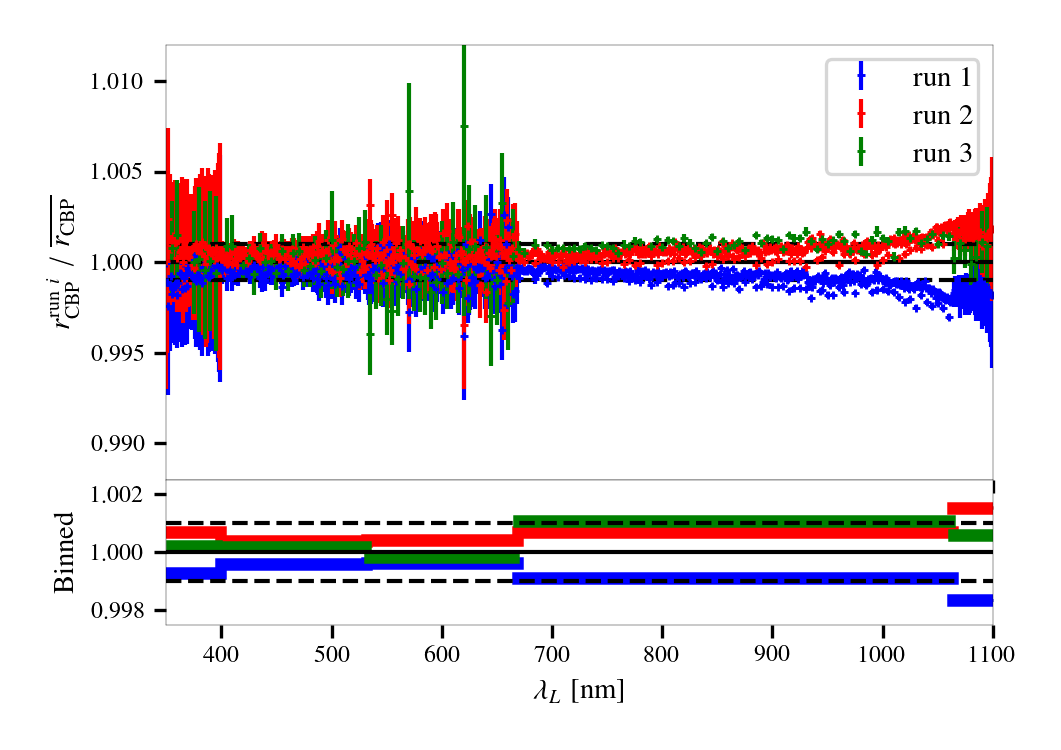
\includegraphics[width=\columnwidth]{fig/sc_runi_ratios.png}
    \caption{Ratios of the CBP charge ratio $r_{\rm CBP}^{\mathrm{run}\ i}\;/\;\overline{r_{\rm CBP}}$ for three different runs as a function of $\lambda_L$. Black dashed lines encompass the per-mil precision region. Top: ratios for each $\lambda_L$. Bottom: binned ratio for four different wavelength ranges.}
    \label{fig:SCrepeatability}
\end{figure}

\subsubsection{Summary}\label{sec:cbp_summary}

In summary, we defined the calibrated amount of charges in the solar cell as:
\begin{equation}
\Qsolarcal \equiv \Qsolarmes - \Qsolar^{\rm dark} - \Qsolar^{532} - \Qsolar^{\lambda_{\rm comp}} - \Qsolar^{\rm fluo}
\end{equation}
and in the photodiode as:
\begin{equation}
\Qphotcal(\lambda_L) = \left\lbrace
\begin{array}{ll}
          \Qphotmes(\lambda_L) - \Qphot^{\mathrm{fluo}}(\lambda_L) &\ \text{if}\ \lambda_L < \SI{400}{\nano\meter} \\
         \Qphotmes(\lambda_L)(1 + \alpha(\lambda_L)) &\ \text{if}\ \lambda_L \in \left[532, 644\right]\mathrm{\,nm} \\
        \Qphotmes(\lambda_L)(1 + \beta(\lambda_L)) &\ \text{if}\ \lambda_L > \SI{1064}{\nano\meter} \\
        \Qphotmes(\lambda_L)&\ \text{elsewhere}
\end{array}\right. 
\end{equation}

All uncertainties from the evaluation of all these terms were propagated. The summary of the error budget on the CBP response is decomposed in Figure~\ref{fig:cbp_budget} as a function of laser wavelength $\lambda_L$. Systematics coming from the wavelength calibration are not represented. Indeed, as the CBP response varies slowly with wavelength, it is negligible compared to others.  In the visible range, scattered light systematics dominates. In the far infrared, the subtraction of the $\lambda_{\mathrm{comp}}$ photons is the main systematic uncertainty, while in the UV range fluorescence correction systematic dominates.

%cbp_paper_plots.ipynb
\begin{figure}[h]
    \centering
    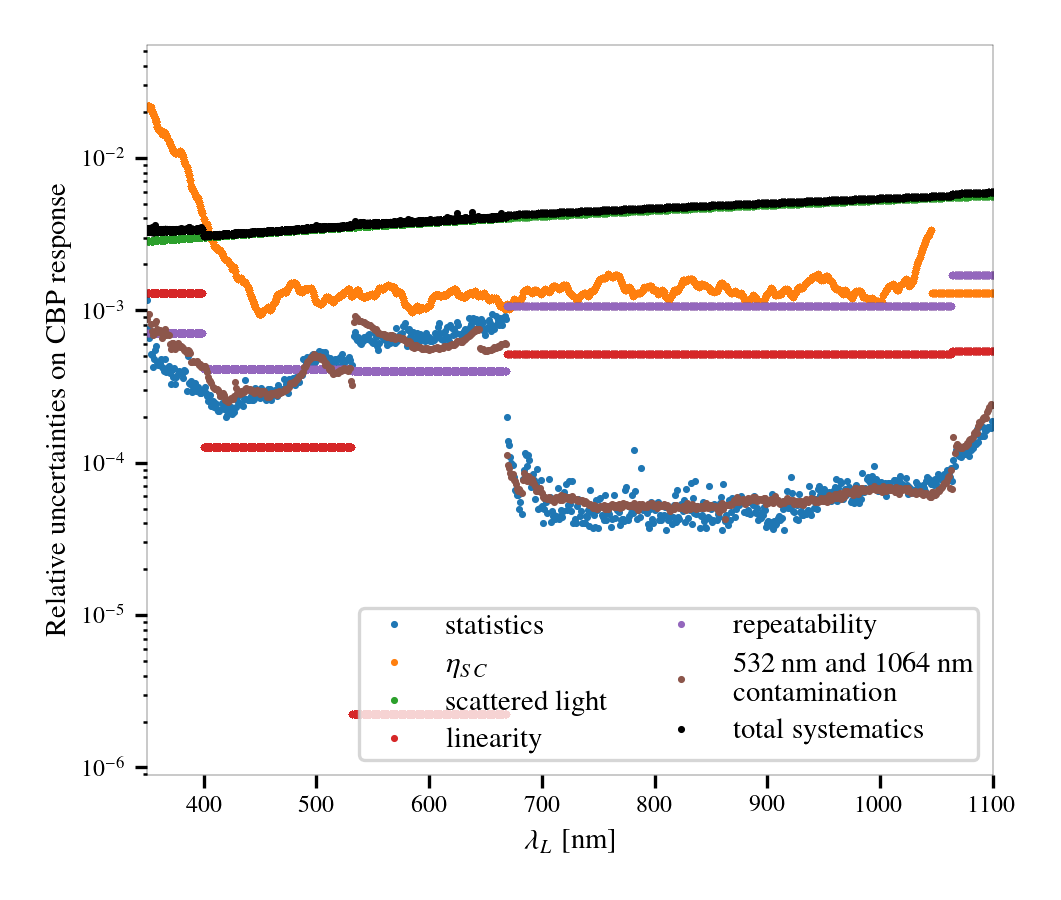
\includegraphics[width=\columnwidth]{fig/cbp_error_budget.png}
    \caption{Total error budget for CBP response.}
    \label{fig:cbp_budget}
\end{figure}

\subsection{CBP response}

The final CBP response in output photons per Coulomb unit in the photodiode is
\begin{equation}
    \Rcbp(\lambda_c) = \frac{\Qsolarcal(\lambda_c)}{\Qphotcal(\lambda_c) \times \epsilon_{\mathrm{solar}}(\lambda_c) \times e}.
    \label{eq:rcbp2}
\end{equation} 
It can be computed for each laser burst. We averaged the values to increase the signal-to-noise ratio and get the red smooth curve presented in Figure~\ref{fig:cbp_response}:
\begin{equation}
    \overline{\Rcbp(\hat{\lambda}_c)} = \left\langle\frac{\Qsolarcal(\lambda_c)}{\Qphotcal(\lambda_c) \times \epsilon_{\mathrm{solar}}(\lambda_c) \times e}\right\rangle_{\lambda_c\in [\lambda,\lambda+\delta \lambda]}.
    \label{eq:rcbp3}
\end{equation} 
The average is performed on every burst of the three runs, with a $5\sigma$ clipping, and $\hat{\lambda}_c$ the mean calibrated wavelength in a $\delta \lambda = \SI{1}{\nano\meter}$ bin. All uncertainties are combined in quadrature (Figure~\ref{fig:cbp_response} bottom).



%cbp_paper_plots.ipynb
\begin{figure}[h]
    \centering
    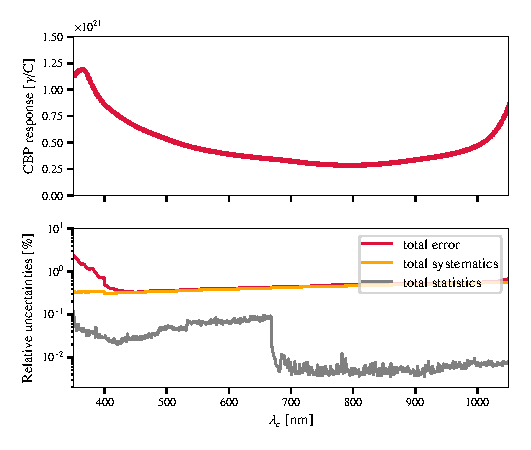
\includegraphics[width=\columnwidth]{fig/cbp_response.pdf}
    \caption{Top: CBP response $\overline{\Rcbp(\hat{\lambda}_c)}$ obtained with the \bpinhole{} pinhole and $\delta \lambda = \SI{1}{\nano\meter}$. Bottom: relative uncertainties.}
    \label{fig:cbp_response}
\end{figure}


%\input{sections/4_instrument_model}
%\clearpage

\section{StarDICE response}
\label{sec:rsd}

In this section, we will show the methodology to obtain the \SD telescope response $\Rtel(\lambda)$ by analyzing \SD camera data.

\subsection{Data set description and strategy}
\label{sec:sd_datadesc}

As described in section \ref{sec:cbp_datadesc}, the laser emits pulses at a rate of \SI{1}{\kilo\hertz} in bursts that are separated with dark times. We set the \spinhole pinhole to measure the \SD throughput and its filter transmissions. Yet, as discussed in Section~\ref{sec:strategy} the calibration of the CBP throughput is obtained with the \bpinhole pinhole, so we use an open transmission measurement of the \SD telescope with both pinholes to intercalibrate the CBP and \SD telescope responses. Figure~\ref{fig:ccd_examples} shows examples of images obtained when the CBP shoots in the \SD CCD camera with two different pinholes. \\

In the following sections, we describe the modelization of the \spinhole pinhole dataset via PSF photometry. Then, we discuss the choice of the baseline photometry used to measure the \SD response, and the method to intercalibrate it with the CBP response. Finally we will show the result obtained.

\begin{figure}[h]
    \centering
    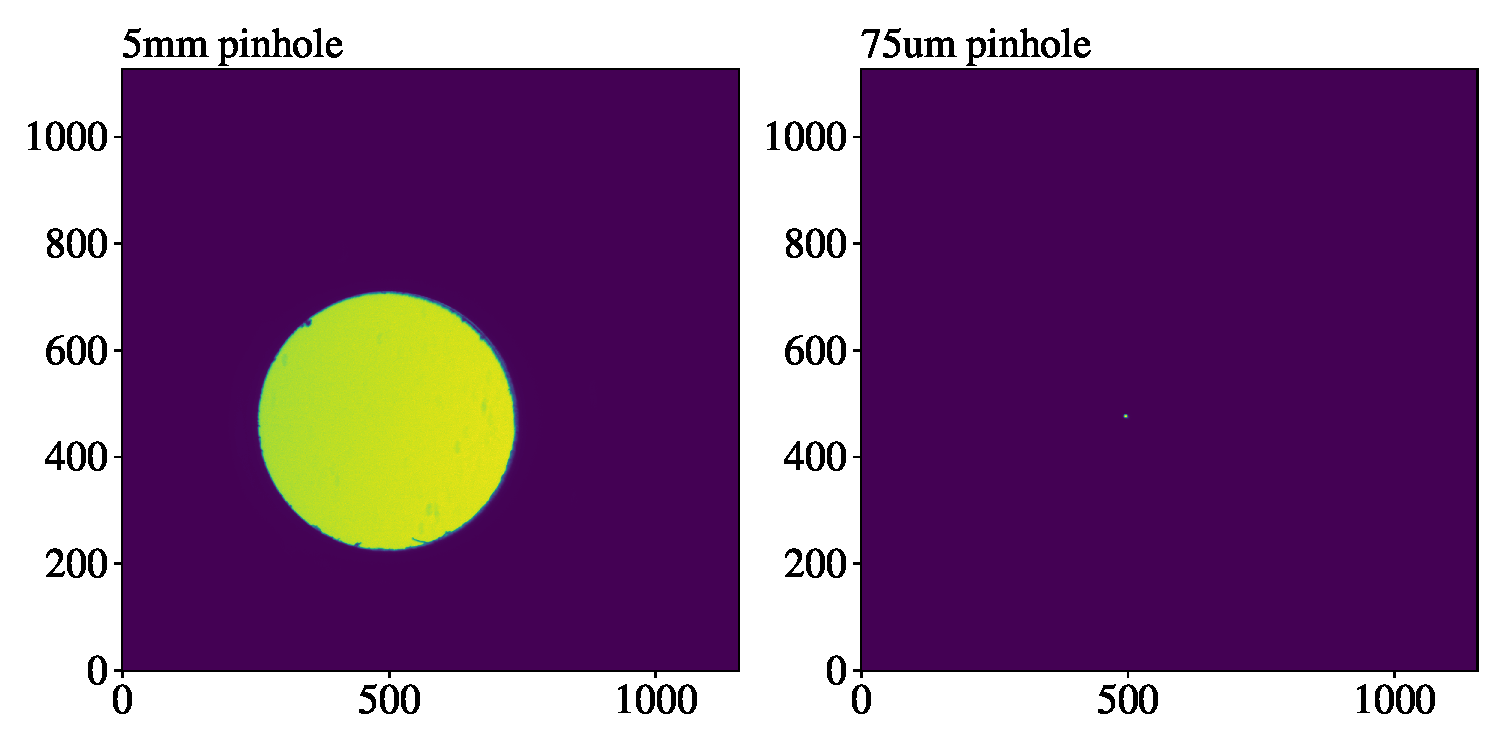
\includegraphics[width=\columnwidth]{fig/ccd_examples.pdf}
    \caption{Examples of images obtained when the CBP shoots in the \SD telescope at $\lambda_L=\SI{450}{\nm}$ with the \bpinhole pinhole on the right and \spinhole pinhole on the left. The ghost reflection is visible for both images at the left of the main spot. In the \bpinhole pinhole image, a large annulus around the main spot is visible, and correspond to light diffusion around a mechanical iris at the input of the CBP.}
    \label{fig:ccd_examples}
    %~/stardice/analysis/cbp_paper/total_fluxes/ghost_stack_figure.ipynb
\end{figure}

\subsection{Overscan subtraction}
\label{sec:overscan}
For both pinholes, the overscan of each image is estimated and subtracted. The mean of each column $i$ of the horizontal overscan and each row $j$ of the vertical overscan is computed. For each pixel $(i, j)$, we subtract the sum of estimation of the overscan estimated on the column $i$ and the row $j$. \\

\subsection{Modelisation of the \SD data for \spinhole pinhole}

%I. model
%difficulté : PSF : convolution ouverture bizarre + réflexions
%on peut modéliser à grande distance : addition moffat + réflexions dans l'optique + ghost 
%description du ghost (2 dans l'infrarouge)
%modélisation courbe de croissance --> plot résultats
%bkg --> cohérent avec darks
%5eme panneau --> chi2/dof

\begin{figure}[h]
    \centering
    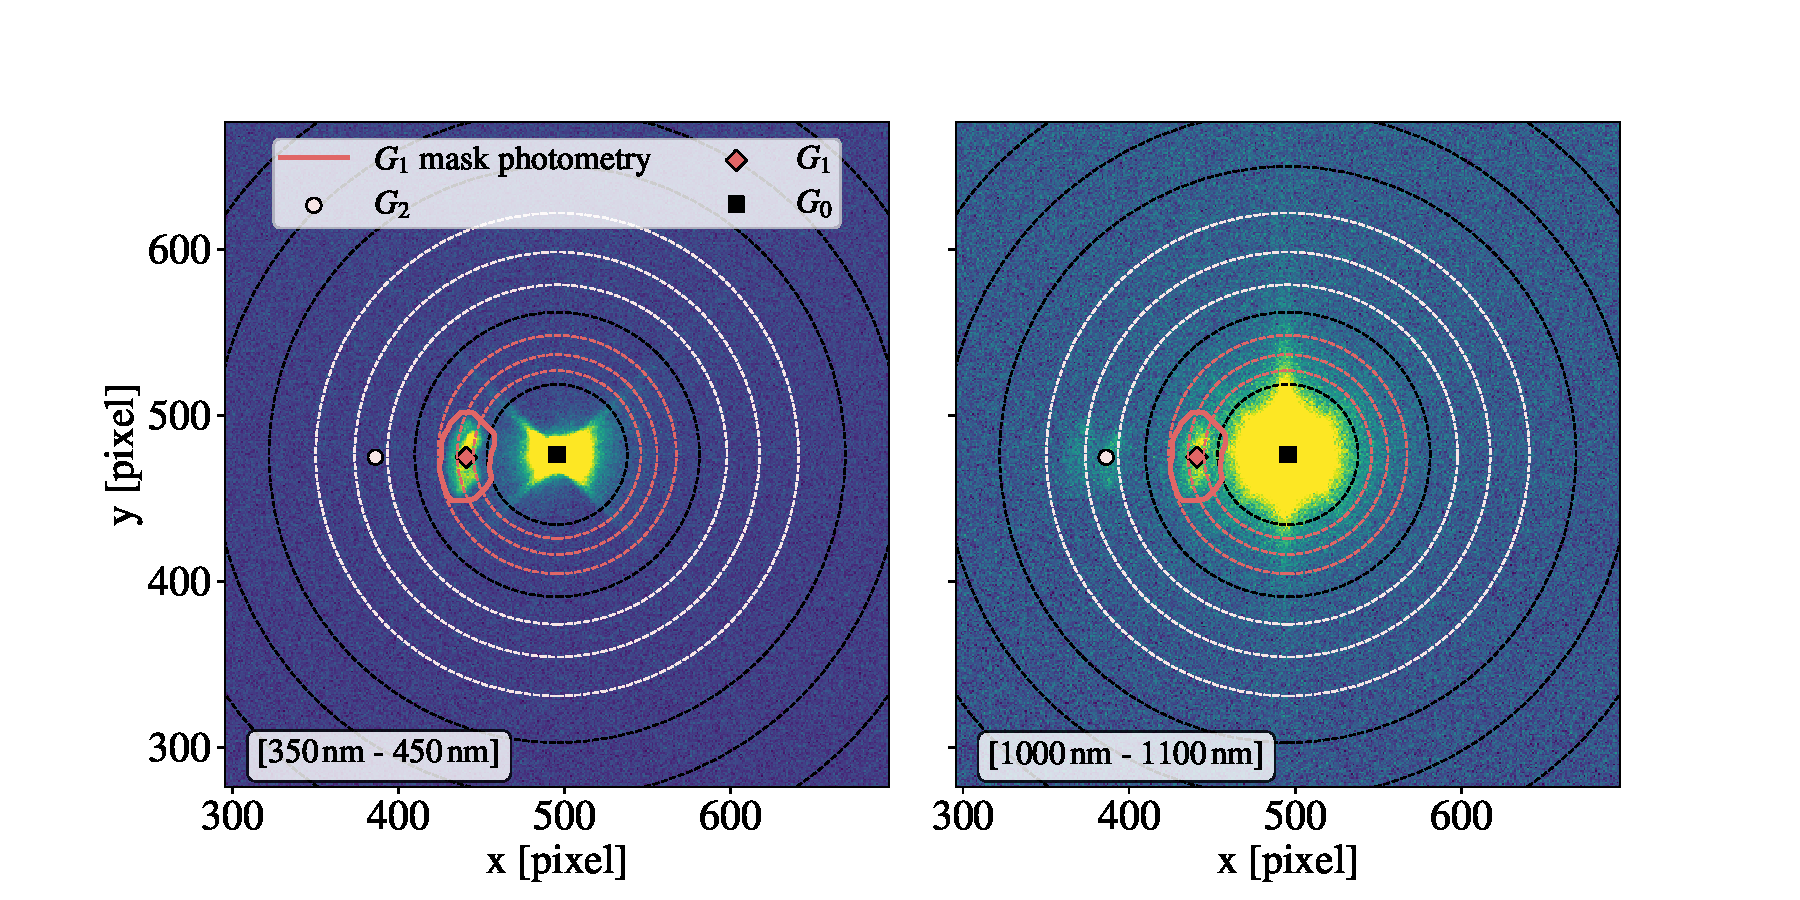
\includegraphics[width=\columnwidth]{fig/ghost_contrast.pdf}
    \caption{Stack of images at different wavelengths, with one image per nanometer. \textit{Left:} Stack of images between \SI{350}{\nano\meter} and \SI{450}{\nano\meter}. The scale is set on the ZScale from IRAF to make faint features visible. The spot of interest $G_0$ is at the center, and the ghost reflections are at its left. The circles correspond to the aperture photometry at different radii, when an annulus contains ghost contribution, it is colored with respect to the order of the ghost. The red area around the 1$\up{st}$ order ghost represents the area where the photometry of the ghost is measured. \textit{Right:} Same image but for a stack of images between \SI{1000}{\nano\meter} and \SI{1100}{\nano\meter}. We note that the 2$\up{nd}$ order ghost is not visible for the stack in the UV, where the 1$\up{st}$ order is maximal, while it is visible in the IR, where the 1$\up{st}$ order is lower. For the stack in IR, we osberve a degradation of the \SD PSF.}
    \label{fig:ghost_contrast}
    %~/stardice/analysis/cbp_paper/total_fluxes/ghost_stack_figure.ipynb
\end{figure}

In this section, we develop a modelization of the \spinhole pinhole dataset, where Figure~\ref{fig:ghost_contrast} shows stacks of images obtained with this dataset. The illumination of a section of the primary StarDICE mirror results in a central image resulting from the \SD telescope PSF, and a set of additional fainter images that we call ghosts. The ghosts result from undesired but unavoidable reflexions on optical surfaces. The most visible ones come from the beam reflexion on the CCD surface and back reflexion on its covering window, as described in Figure~\ref{fig:schema_ghost}.\\

We consider that the \SD telescope PSF can be modelized as a Moffat distribution \citep{moffat} $M(r, \lambda)$ which depends on the radius $r$ and the wavelength $\lambda$ as:

\begin{equation}
M(r, \lambda)= 1 - \left( 1+\frac{r^2}{\alpha(\lambda)^2} \right)^{1-\beta(\lambda)},
\end{equation}
with $\alpha(\lambda)$ and $\beta(\lambda)$ the parameters of the Moffat distribution. The flux $F(r, \lambda)$ measured in the CCD with aperture photometry, can be modelized as: 

%Thus, the core of the spot in the CCD is the convolution of the PSF, the CBP output shape, and ghosts from light reflections between the glass before the CCD and the CCD itself, as schematized in Figure~\ref{fig:schema_ghost}. These contributions make the core of the spot complex to model. However the tail of the PSF should not be impacted by the contribution of the CBP output shape and the light diffusion, so it is expected to behave like a Moffat distribution. 

\begin{equation}
F(r, \lambda) = A(\lambda) \times \frac{M(r, \lambda) + \Kghostfit(r, \lambda)}{1 + \Kghostfit(r \rightarrow +\infty, \lambda)} + \bkg(r, \lambda),
\label{eq:moffat_model}
\end{equation}
with $A(\lambda)$ the total amplitude, $\Kghostfit(r, \lambda) = \frac{\sum_{n=1}^{+\infty} G_n(\lambda)}{A(\lambda)}$ the relative contribution of the sum of all the ghosts $G_n(\lambda)$ and $\bkg(r, \lambda)$ the contribution of the background. The origin of the ghost contribution is schematized in Figure~\ref{fig:schema_ghost}.

The fit is done with PSF photometry for a radius $r=\SI{20.9}{pixels}$, and then for successive annulus of external radius from \SI{24.9}{pixels} to \SI{419.1}{pixels}. These radii are regularly spaced on a logarithm scale shown in Figure~\ref{fig:ghost_contrast}. The parameters of the fit are adjusted with the \spinhole pinhole dataset No.~8 from Table~\ref{tab:schedule}, with one image per wavelength. To take into account $\Kghostfit(r, \lambda)$, an additive value is fitted for every annulus that contains a ghost contribution. The evolution of the Moffat distribution is expected to be smooth with respect to wavelength, so the parameters $\alpha(\lambda)$ and $\beta(\lambda)$ are developed on a B-spline basis with 15 wavelength nodes regularly spaced between \SI{350}{\nano\meter} to \SI{1100}{\nano\meter}. The same goes for the function $\Kghostfit(r, \lambda)$ as it corresponds to light reflections on surfaces in the optical path. The results of this fit are shown Figure~\ref{fig:result_params}. 

\begin{figure}[h]
    \centering
    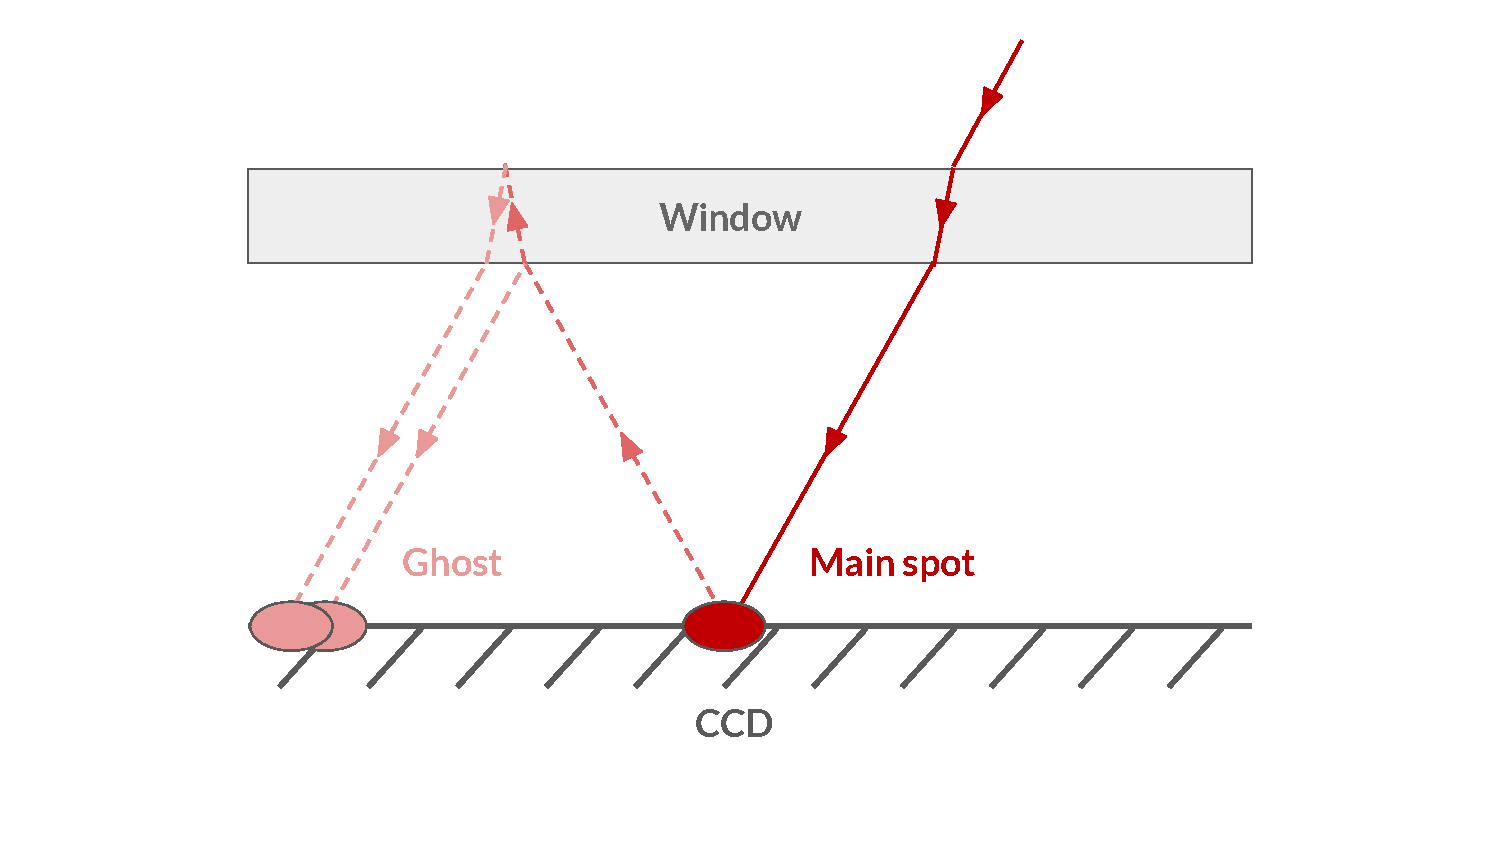
\includegraphics[width=\columnwidth]{fig/schema_ghost.pdf}
    \caption{Schematic of the light reflections that generate the ghosts, which are defocused and less intense images at other positions in the focal plane. A fraction of the light is reflected at the different interfaces and $G_0(\lambda)$, $G_1(\lambda)$ and $G_2(\lambda)$ are respectively the main spot, the 1\up{st} order ghost, and the 2\up{nd} order ghost.}
    \label{fig:schema_ghost}
    %Google slides
\end{figure}

In the first and second panel, we can see that the $\alpha(\lambda)$ and $\beta(\lambda)$ parameters of the PSF are stable within \SI{350}{\nano\meter} and \SI{900}{\nano\meter}, and change significantly beyond. This is correlated with a change of the PSF shape in the infrared as can be seen in the image stacks in Figure~\ref{fig:ghost_contrast}. 

The third panel shows a constant background against wavelength, with a mean of $\mu_\mathrm{bkg, fitted}=\SI{0.267}{ADU/pixel}$ for an exposure time of \SI{1.1}{\second}. This panel show also the result of an independant study of the background analyzing dark images. Two datasets of dark images have been studied, one with the laser turned off, and a second by masking the CBP output with a cap (dataset No.~9 in Table~\ref{tab:schedule}). Both datasets are constants in time and wavelength, and their mean value of ADU/pixel are compatible, so we combine them into one dataset of darks. The mean photometry value of this dataset is represented by the black dashed line in this third panel, and is $\mu_\mathrm{dark, photometry}=\SI{0.252}{ADU/pixel}$ with a standard deviation $\sigma_\mathrm{dark, photometry}=\SI{0.059}{ADU/pixel}$. We conclude that the estimation of the background with the fit is consistent with the dark datasets results. \\

The fourth panel presents the relative contribution of the first order ghost $G_1(\lambda)$, $\Kghostfitfirst(\lambda) = \frac{G_1(\lambda)}{A(\lambda)}$ in percent, superimposed with the fraction $\Kghost=\frac{G_1(\lambda)}{G_0(\lambda)}$ obtained by photometry measurements on the first order ghost $G_1(\lambda)$ and the main spot $G_0(\lambda)$. The method to perform ghost photometry is detailed in Appendix~\ref{sec:ghost_photometry}. The ratio $\Kghost$ and $\Kghostfitfirst$ obtained with two different methods on two different datasets are superimposing well below \SI{950}{\nano\meter}, which gives us confidence about the accuracy of this measurement. The deviation above \SI{950}{\nano\meter} between the two methods can be explained by the following arguments. the $\alpha(\lambda)$ and $\beta(\lambda)$ parameters indicate a deterioration of the PSF, which starts to overflow in the ghost photometry. In addition, interference fringes are appearing in the focal plane at these wavelengths, complicating the ghost photometry. As the fit accounts for the PSF evolution, the fitted result gives more confidence in its accuracy.

The reduced chi-squared of the fit in the fifth panel reach a value close to 1 at every wavelength, which indicates that the model satisfactorily describes the dataset.

\begin{figure}[h]
     \centering
     \resizebox{\hsize}{!}{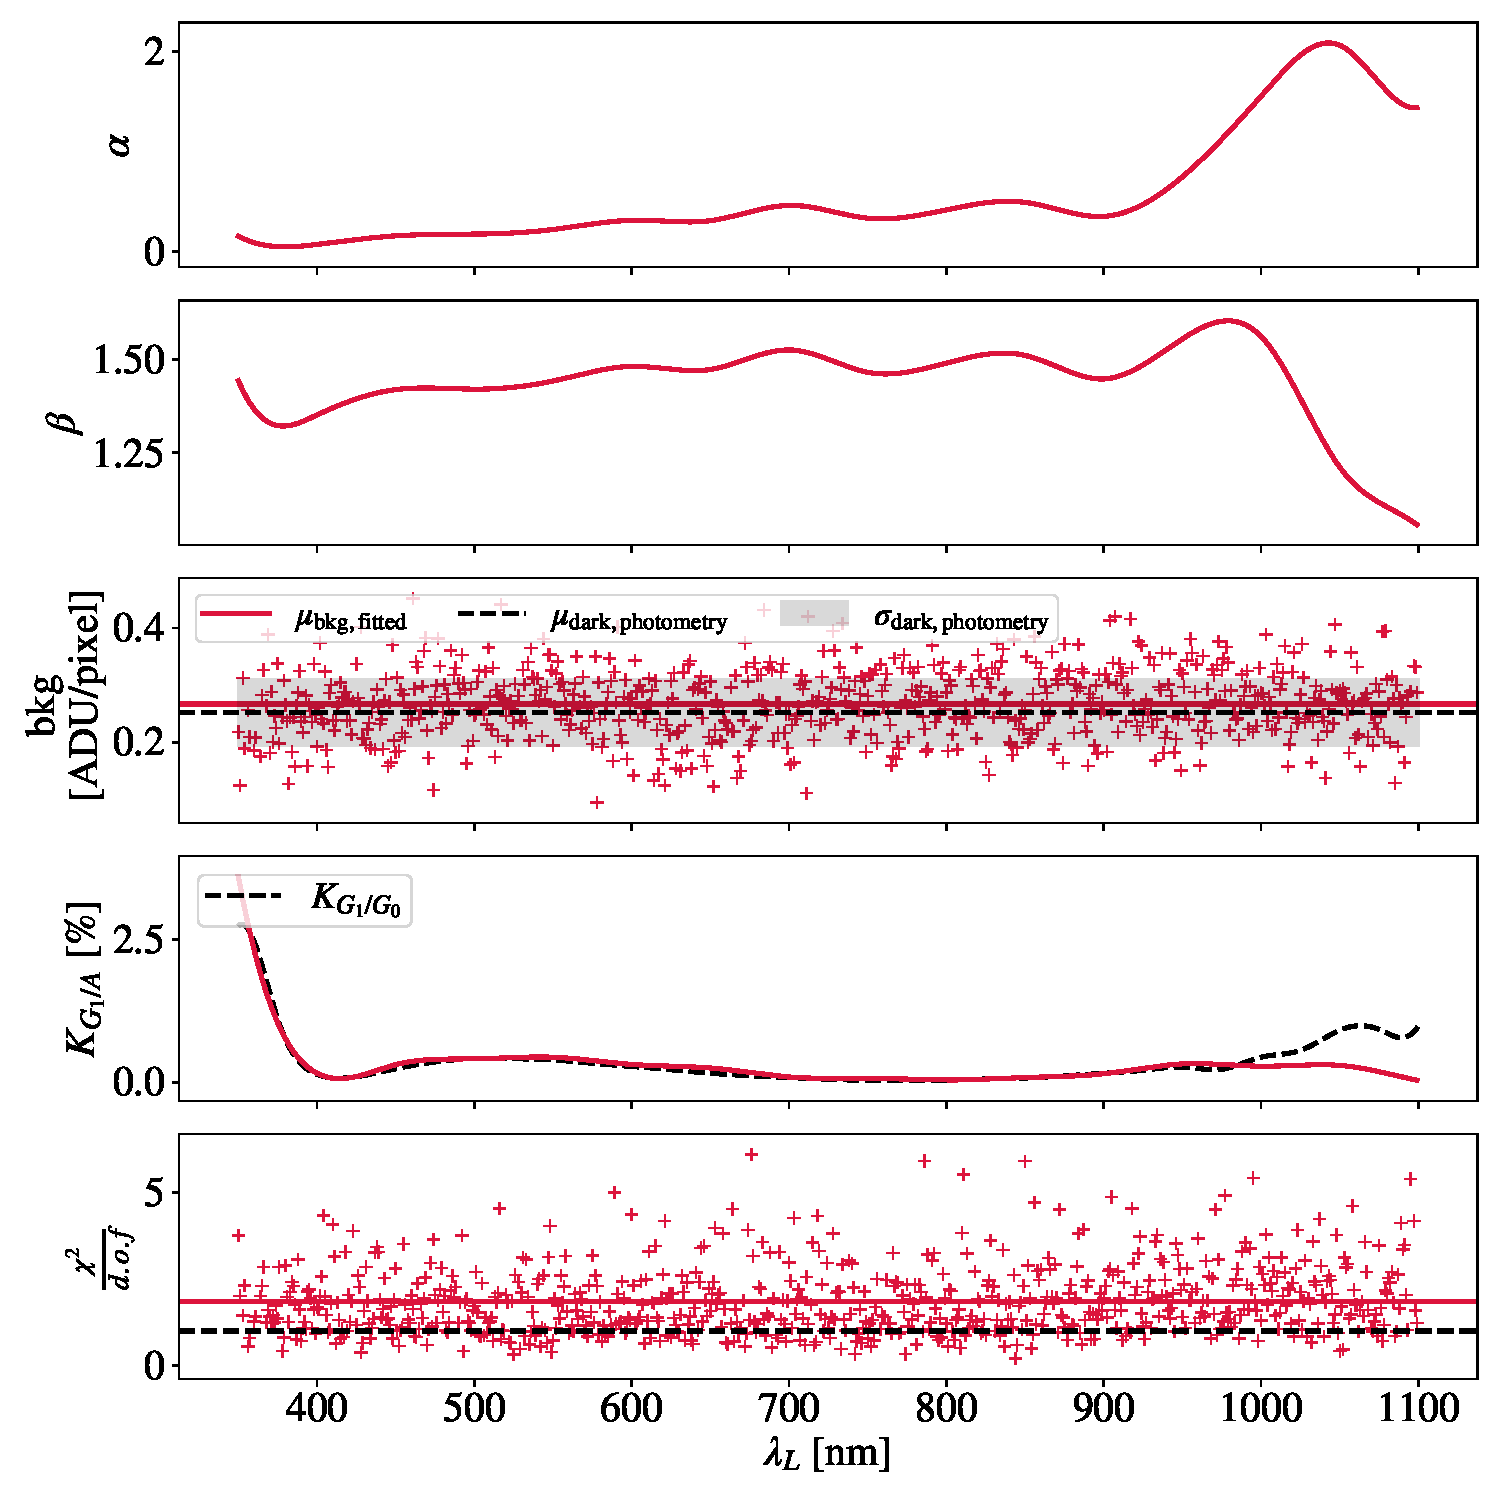
\includegraphics{fig/result_params.pdf}}
     \caption{Best fitting parameters for the model of Equation~\ref{eq:moffat_model}. Red plain lines correspond to the result of the fit, and black dashed lines to the values expected. From top to bottom: the first and second panel represent respectively the $\alpha(\lambda)$ and $\beta(\lambda)$ parameters from the Moffat distribution; the third panel shows the background contribution per pixel and its mean value in red, while the dark dashed line is the mean value of the dark; the fourth panel represents $\Kghostfitfirst(\lambda)$, and $\Kghost$; the fifth panel represents the reduced chi-squared of the fit.}
     \label{fig:result_params}
    %~/stardice/analysis/cbp_paper/total_fluxes/fit_results.ipynb
\end{figure}

%II. photométrie portable sur ciel 
%
%on peut modéliser pcq on n'a pas de fond --> propre aux images CBP (pas de fond ciel, source isolée), donc peut pas faire en pratique sur ciel
%
%comme d'hab : soustraction de fond classique et se limiter à ouverture donnée ~20 pixels
%si on fait ça, voilà la fraction du flux qu'on récupère : plot de correction d'ouverture phi20/A (quantifier les biais sur F(20)/A et ap_bkg ou fit_bkg), biais à cause du flux perdu et biais à cause de la source  
%
%Problèmes IR:
%1) params fitté partent aux fraises dans l'IR, ça doit venir de StarDICE, peut-être transparence du télescope (regarder dans le filtre y comparé au filtre g ou i) --> peut pas reconstruire de manière précise le flux d'une étoile au-delà de 1000nm (pas de lien entre CBP et obs stardice)
%
%On va mesurer l'ensemble des spots CBP avec l'ouverture à 20 pixels sachant que dans l'IR c'est pas fou 
%*98\% du flux stable en couleur

\subsection{Photometry for filter throughput measurement}
\label{sec:photometry_small}

The modelization of the PSF at long distance from its core is possible because of the laboratory conditions of these images. These conditions are intrisinc to CBP images, with an isolated source and no sky background. It is impossible to port this method with on-sky data. We choose to carry out the whole analysis with aperture photometry and a background estimation reproducible with on-sky data. This method is the baseline photometry for the \spinhole pinhole, and we compared the measurements obtained with such a method and the fitted parameters to quantify eventual biases. 

\subsubsection{Background subtraction}
\label{sec:bkg}

To estimate the background contribution, the sources in the image need to be detected and masked. We compute the standard deviation of an image $\sigma$, and every pixel with a signal higher than 5$\sigma$ is masked, as well as all the surrounding pixels that has a signal higher than 2$\sigma$. Then we proceed to a segmentation of the masked image into boxes of $129\times132$ pixels. We compute the mean and the standard deviation of the background in each of these boxes, and we interpolate their values in a 2D map to get our estimation of the background. This background estimation is subtracted to the image. Then, the centroid of the spot of interest is computed to pursue aperture photometry at this position. $\Qccd$ is measured with aperture photometry at a radius of \SI{20.9}{pixels} for every image of the dataset with the \spinhole.

\subsubsection{Correction of the light contamination}\label{sec:sd_contaminations}

When measuring the flux collected from the \SD camera, we have to remove light contaminations described in Sections~\ref{sec:532_cont} and~\ref{sec:fluorescence}. As the photodiode and the solar cell, the total signal measured in the \SD camera $\Qccdmes$ is the sum of the flux from the main laser line $\Qccdcal$ and the flux from the \SI{532}{\nm} contamination $\Qccd^{532}$, the $\lambda_{\rm comp}$ contamination $\Qccd^{\lambda_{\rm comp}}$, and the integrating sphere fluorescence $\Qccd^{\mathrm{fluo}}$, as follows:
\begin{equation}
    \Qccdmes = \Qccdcal + \Qccd^{532} + \Qccd^{\lambda_{\rm comp}} + \Qccd^{\mathrm{fluo}}
    \label{eq:qccd_mes}
\end{equation}

The contamination light in the \SD camera can be estimated by multiplying $\Qphot^{532}$, $\Qphot^{\lambda_{\rm comp}}$ and $\Qphot^{\mathrm{fluo}}$ by $\Rcbp(\lambda)$ and $\Rtel(\lambda)$. The contaminations are subtracted, and impact on filter transmission measurement is shown Figure~\ref{fig:g_filter_532}, focusing on the \SD g filter, the most affected filter by integrating sphere fluorescence and \SI{532}{\nano\meter} line.

\begin{figure}[h]
    \centering
    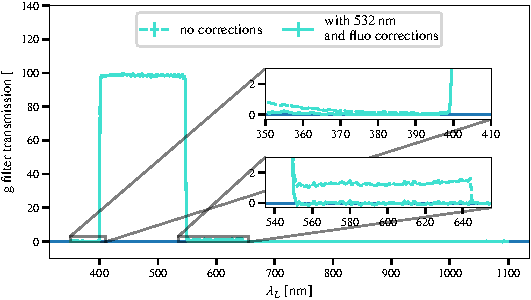
\includegraphics[width=\columnwidth]{fig/g_filter_532.pdf}
    \caption{\SD g filter transmission as a function of the set laser wavelength $\lambda_L$, with and without the \SI{532}{\nm} and fluorescence correction. For clarity, we added a zoom on the out-of-band transmission where $\SI{532}{\nm}$ line is transmitted while higher wavelengths are shot by the laser.}
    \label{fig:g_filter_532}
    %cbp_paper_plots.ipynb
\end{figure}

\subsubsection{Aperture correction}

In this section, we aim to quantify the fraction of flux missed when measuring the signal for a \spinhole pinhole image with aperture photometry rather than with the PSF photometry. We define the faction of flux missed as the ratio between the value measured with photometry for a given radius and the total amplitude $A$ fitted for a given wavelength. It is quantified in Figure~\ref{fig:bias_aperture}. Less than 3\% of the flux is missed between \SI{400}{\nano\meter} and \SI{900}{\nano\meter}. Below \SI{400}{\nano\meter} the ghost contribution is missed when using an aperture of \SI{20.9}{pixels}. Above \SI{900}{\nano\meter} where the PSF is degrading, the fraction of flux missed increase by one order of magnitude and reach more than 75\%. The bottom panel of Figure~\ref{fig:bias_aperture} shows that the baseline photometry is compatible to the fit estimation at less than 0.2\% between \SI{400}{\nano\meter} and \SI{900}{\nano\meter}. 

\begin{figure}[h]
     \centering
     \resizebox{\hsize}{!}{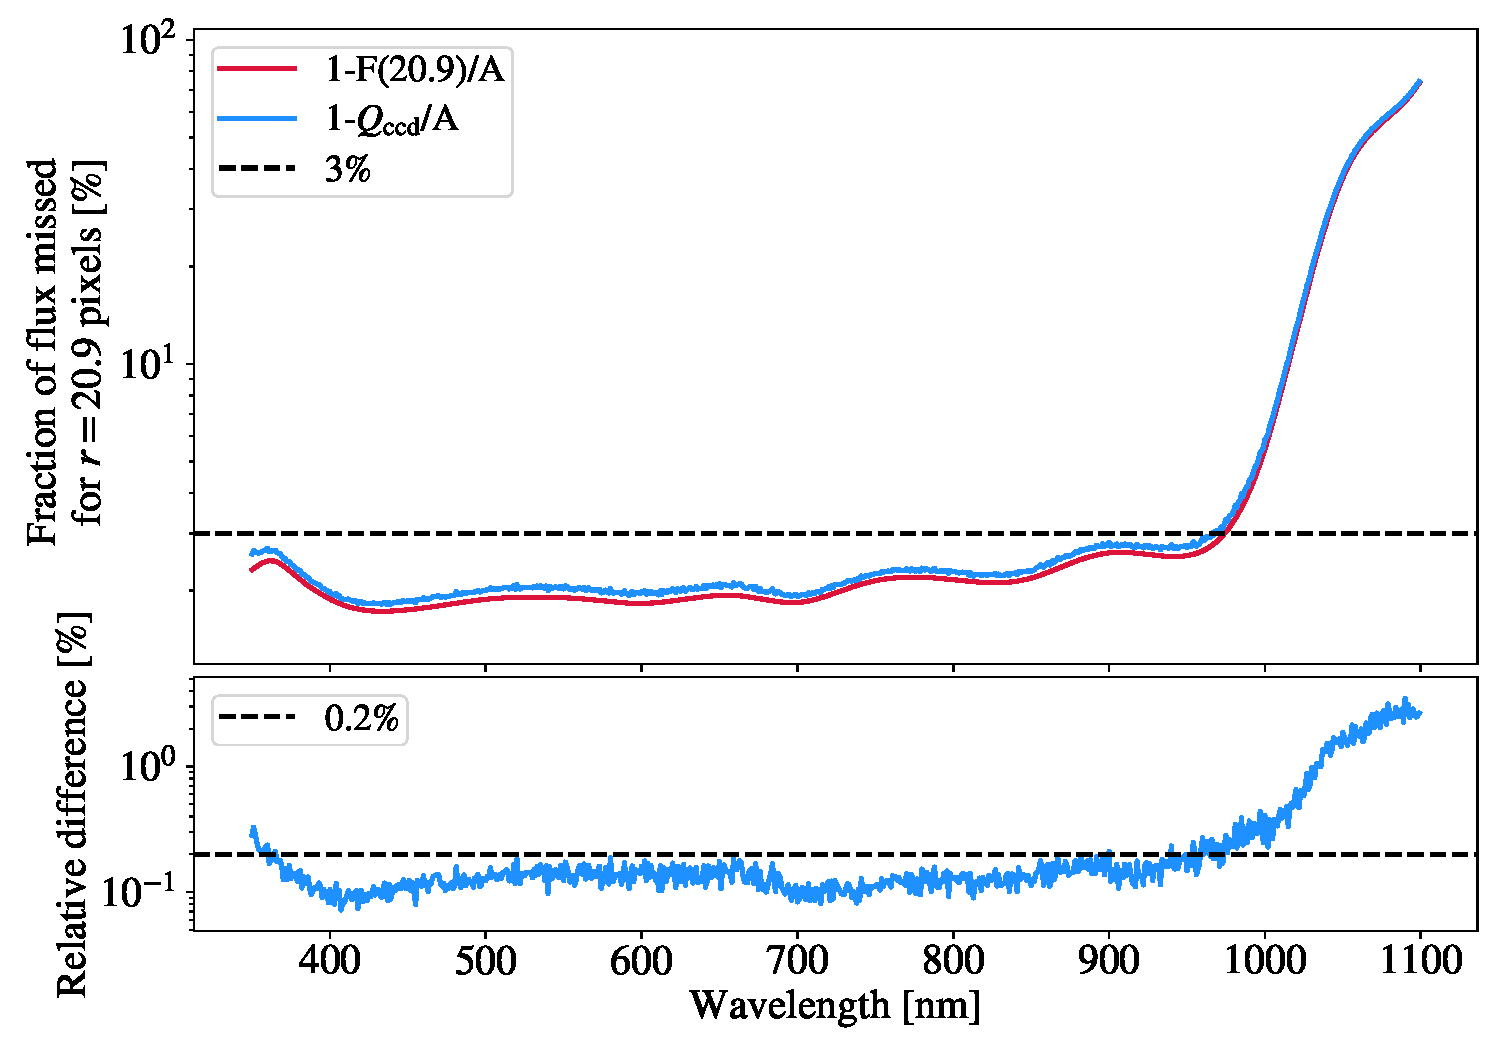
\includegraphics{fig/bias_aperture.pdf}}
     \caption{\textit{Top:} Fraction of missing flux against $\lambda_L$ when measuring \spinhole pinhole dataset with aperture photometry at \SI{20.9}{pixels} rather than taking the total amplitude $A$ fitted. The red curve corresponds to the estimation of the fit, the green one to aperture photometry when the backgruond is estimate with the dark datasets, and the blue one to aperture photometry when the background is estimate with the method described in Section~\ref{sec:photometry_small}. \textit{Bottom:} Relative difference in percent between the flux measured for aperture photometry with the two background estimations and the model estimation at \SI{20.9}{pixels}.}
     \label{fig:bias_aperture}
    %~/stardice/analysis/cbp_paper/total_fluxes/fit_results.ipynb
\end{figure}

We can reach the conclusion that the baseline aperture photometry for the \spinhole pinhole can be used for the range between \SI{400}{\nano\meter} and \SI{900}{\nano\meter}. Below \SI{400}{\nano\meter} there is a need to take care of the ghost contribution. Above \SI{900}{\nano\meter}, this method does not measure a representative flux of the target. It is believed that the \SD telescope is the one responsible for the PSF degradation, one possible explanation is that the primary mirror is becoming partially transparent and generate defocused light. Anyhow, the CBP measurements cannot be trusted in this wavelength range. 

\subsubsection{Pinhole intercalibration}

It is necessary to intercalibrate the \SD response measurements obtained with the \spinhole pinhole with the CBP response measurements obtained with the \bpinhole pinhole. To link these measurements, we measure the \SD responses with the \spinhole pinhole and the \bpinhole pinhole and compute the pinholes ratio $\Kpinholes$. This ratio is defined such as the $\Rcbp$ defined in Equation~\ref{eq:rsd} is the \spinhole pinhole CBP response $\Rcbp^{\spinhole}$, which can be obtained with the \bpinhole pinhole CBP response $\Rcbp^{\bpinhole}$:

\begin{equation}
	\Rcbp(\lambda) \equiv \Rcbp^{\spinhole}(\lambda) = \Rcbp^{\bpinhole}(\lambda) \times \Kpinholes
\end{equation}

When shooting with the \bpinhole pinhole, the main spot is not a pointlike source, hence the data reduction of $\Qccd^{\bpinhole}$ is different than the baseline photometry. The overscan subtraction and the light contamination correction are done with the same method than the \spinhole pinhole, detailed respectively in \ref{sec:overscan} and \ref{sec:sd_contaminations}. However the background subtraction cannot be performed the same way. 

When using \bpinhole pinhole, the main spot takes a significant area of the focal plane, meaning there is not enough background in the image to reconstruct it. The background is measured with dark exposures with the dark datasets mentioned above, and the spatial mean of all these dark images is computed to obtain a master dark. The background contribution is estimated by aperture photometry in the master dark at the same position and same radius than the laser-on images. $\Qccd^{\bpinhole}$ is measured with aperture photometry, after background subtraction. The optimal radius is evaluated at 300 pixels for the \bpinhole pinhole in order to contain the main spot and the 1\up{st} order ghost. We could have increased the radius to contain the iris flux, but it would have added as much noise as the signal gained. 

To compare the \SD responses for both pinhole, we need to measure the fluxes with aperture photometry at the same radius so that it contains the same features, such as the ghost contribution. This way there is no other consideration than the geometry of the pinholes. We estimate the \spinhole pinhole flux $F(300, \lambda)$, $\Qccd^{\bpinhole}$ with the method described in Section~\ref{sec:photometry_big}. We compute the ratio $\Kpinholes=\frac{F(300)}{\Qccd^{\bpinhole}}$ and show the result in Figure~\ref{fig:ratio_pinholes}. The linear fit of this ratio is used to intercalibrate the \bpinhole pinhole $\Rcbp(\lambda)$ obtained and the \spinhole pinhole \SD for every measurements of this analysis.

%The non-null slope and not expected as the ratio between the two pinholes should corresponds only to the ratio of surfaces of illuminated area at the input CBP. We suspect that some light diffusion on the edges of the pinholes or other complex reflections in the setup could give this ratio a chromatic dependance.


\begin{figure}[h]
    \centering
    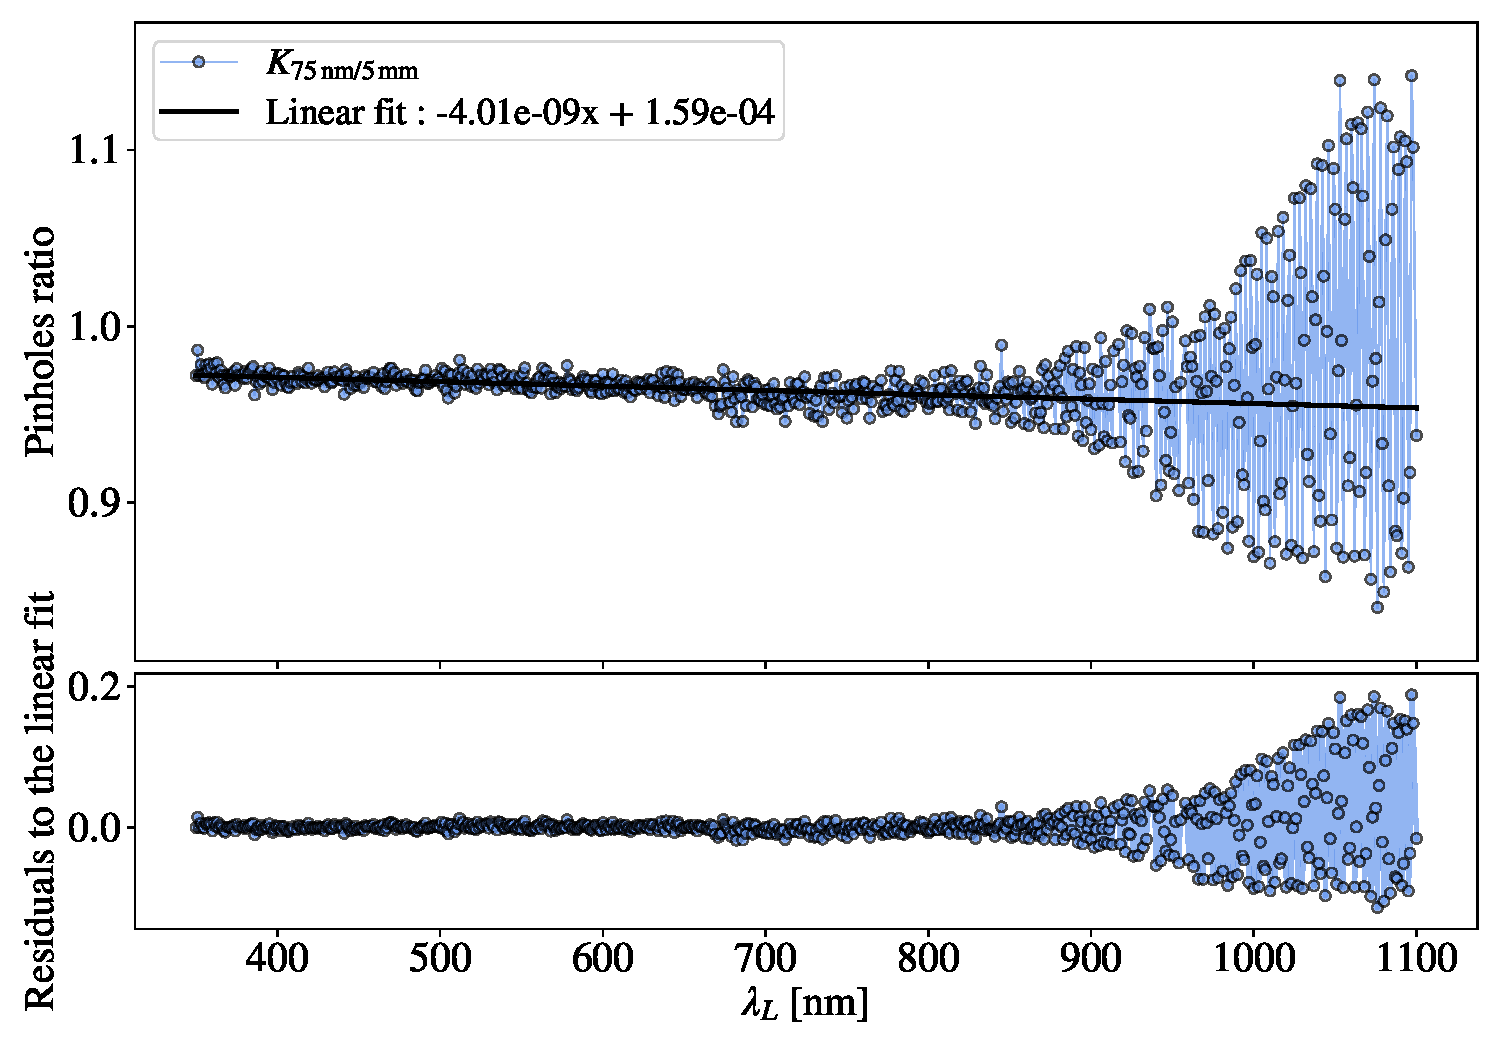
\includegraphics[width=\columnwidth]{fig/ratio_pinholes.pdf}
    \caption{Ratio $\Kpinholes$ with respect to wavelength. The black line corresponds to a linear fit between \SI{400}{\nm} and \SI{900}{\nm}.}
    \label{fig:ratio_pinholes}
    %~/stardice/analysis/cbp_paper/total_fluxes/ratio_pinholes.ipynb
\end{figure}

% The bottom panel corresponds to the aperture correction that is needed to apply to the aperture photometry measurement. It is around 2\% below \SI{950}{\nano\meter}, and increase by one order of magnitude in the infrared. This increase is correlated with the variation of the Moffat parameters $\alpha$ and $\beta$, showing that the PSF is drastically changing in the near infrared. This issue is discussed in more details section \ref{sec:ir}. The third panel show a constant background against wavelength, at a mean of \SI{0.27}{ADU/pixel}.
%
%\subsubsection{Summary}
%
%The summary of the error budget on the \SD telescope response id detailed in Figure~\ref{fig:sd_budget}
%
%
%\begin{figure}
%    \centering
%    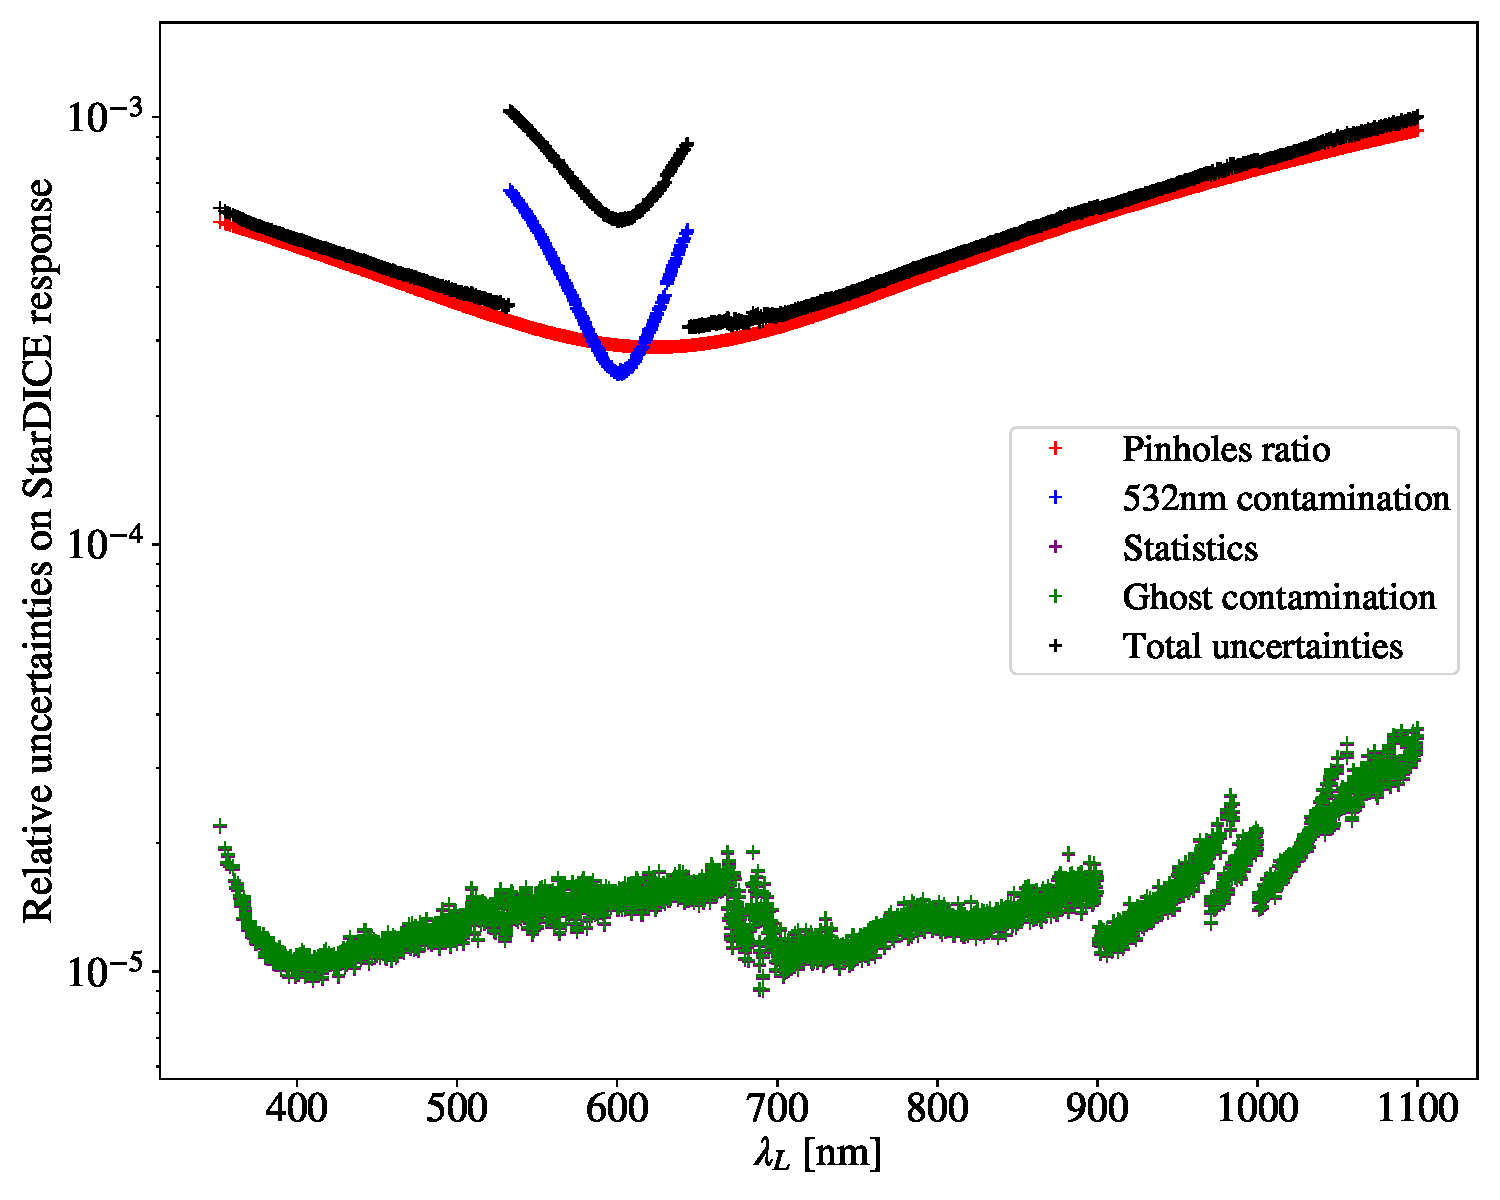
\includegraphics[width=\columnwidth]{fig/sd_uncertainties_budget.pdf}
%    \caption{Total error budget for \SD response.}
%    \label{fig:sd_budget}
%\end{figure}

\subsection{\SD response}

In this section we present the results obtained for the \SD throughput measurement with the \bpinhole pinhole from dataset No.~8; the StarDICE throughput and its filter and grating transmissions measurement with the \spinhole pinhole from dataset No.~6; and the measurements of the datasets No.~2, No.~3 and No.~12. 

\subsubsection{\SD throughput with \bpinhole pinhole}

The Figure~\ref{fig:stardice_5mm_response} show the \SD response obtained with the \bpinhole pinhole, and no filter.

\begin{figure}[h]
    \centering
    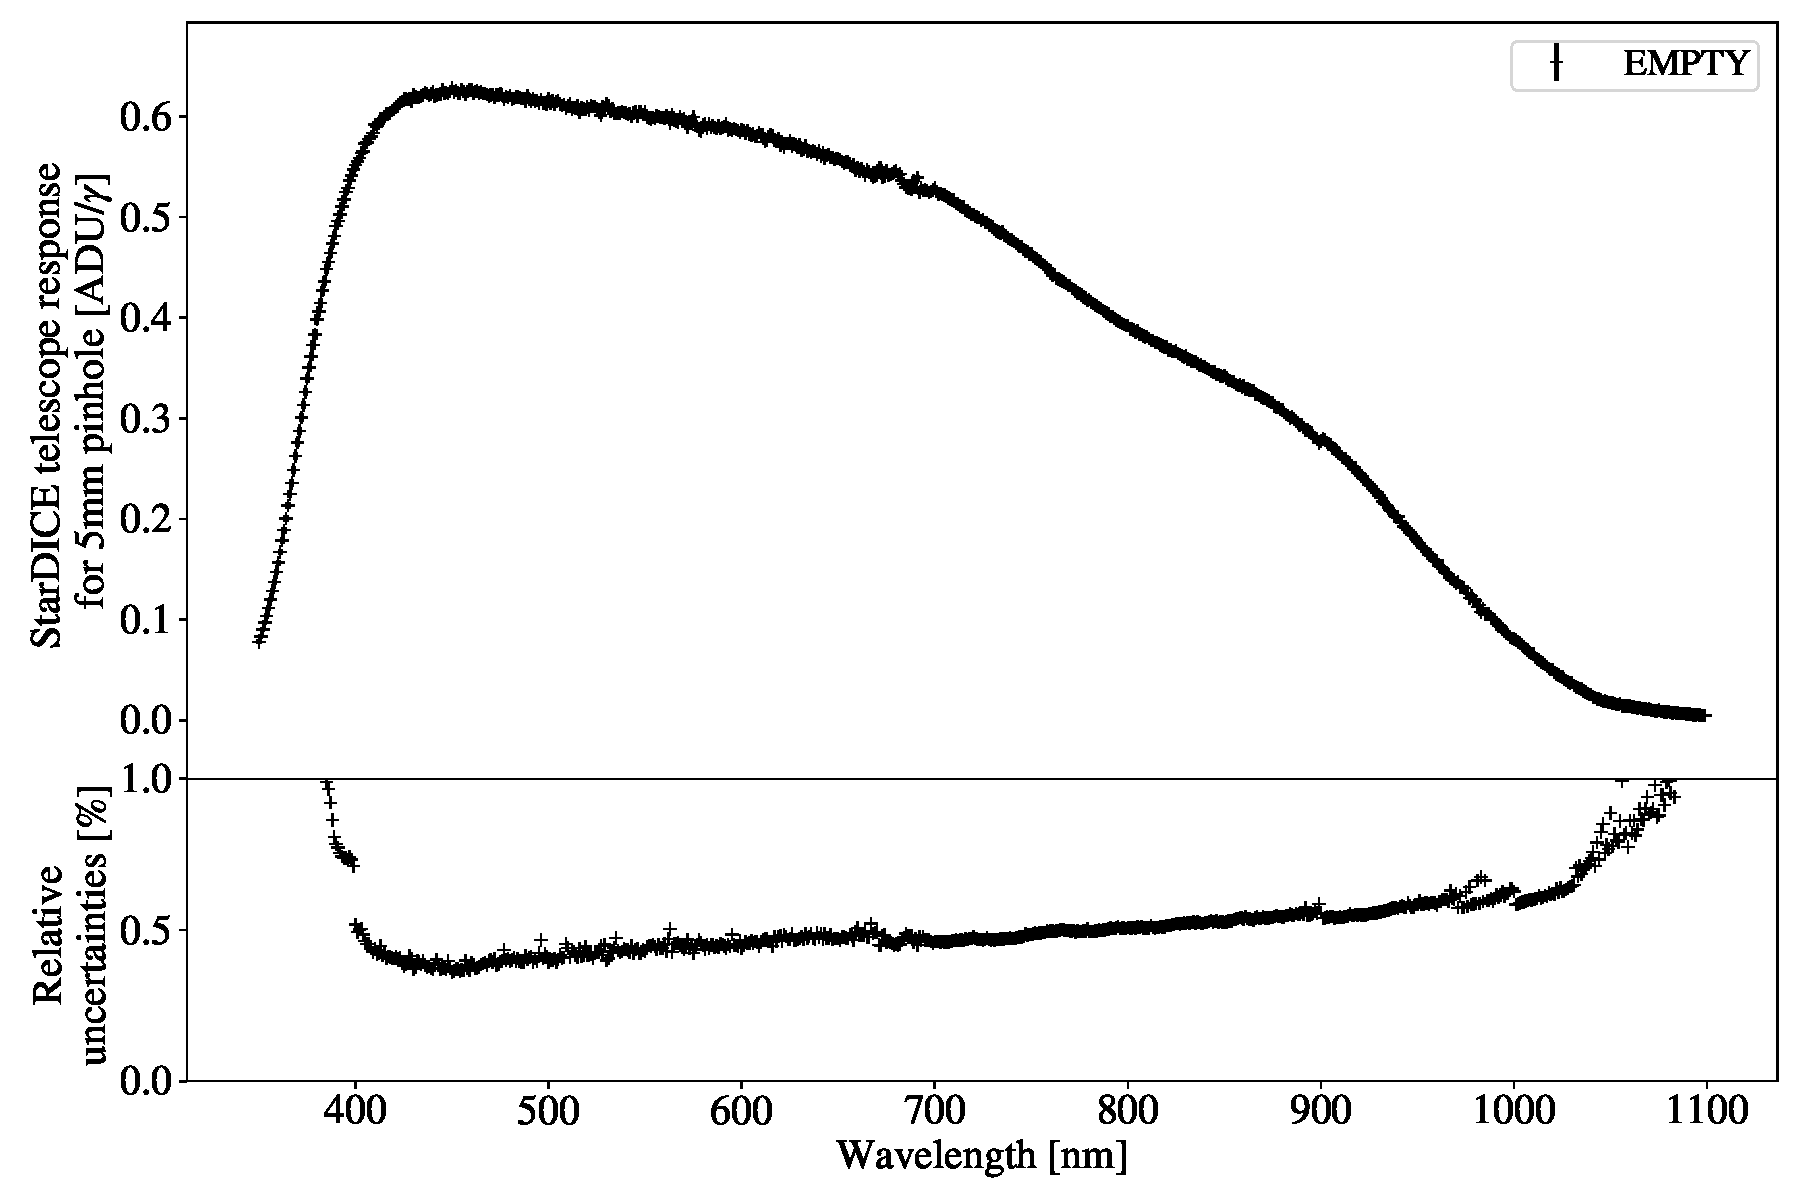
\includegraphics[width=\columnwidth]{fig/stardice_5mm_response.pdf}
    \caption{\textit{Top:} \SD response with no filter and \bpinhole pinhole with respect to wavelength in nanometer. \textit{Bottom:} Uncertainties over the \SD response measurement with respect to wavelength in nanometer.}
    \label{fig:stardice_5mm_response}
    %~/stardice/analysis/cbp_paper/golden_sample_analysis/dr2/response_plots.ipynb
\end{figure}

\subsubsection{\SD throughput and filter transmissions with \spinhole pinhole}

The Figure~\ref{fig:stardice_75um_response} show the \SD response obtained with the \spinhole pinhole, with all filters. In this figure can see that the wavelength resolution is precise enough to have several points in the filter edges, which is a good feature to measure precisely the filter central wavelength. 

\begin{figure}[h]
    \centering
    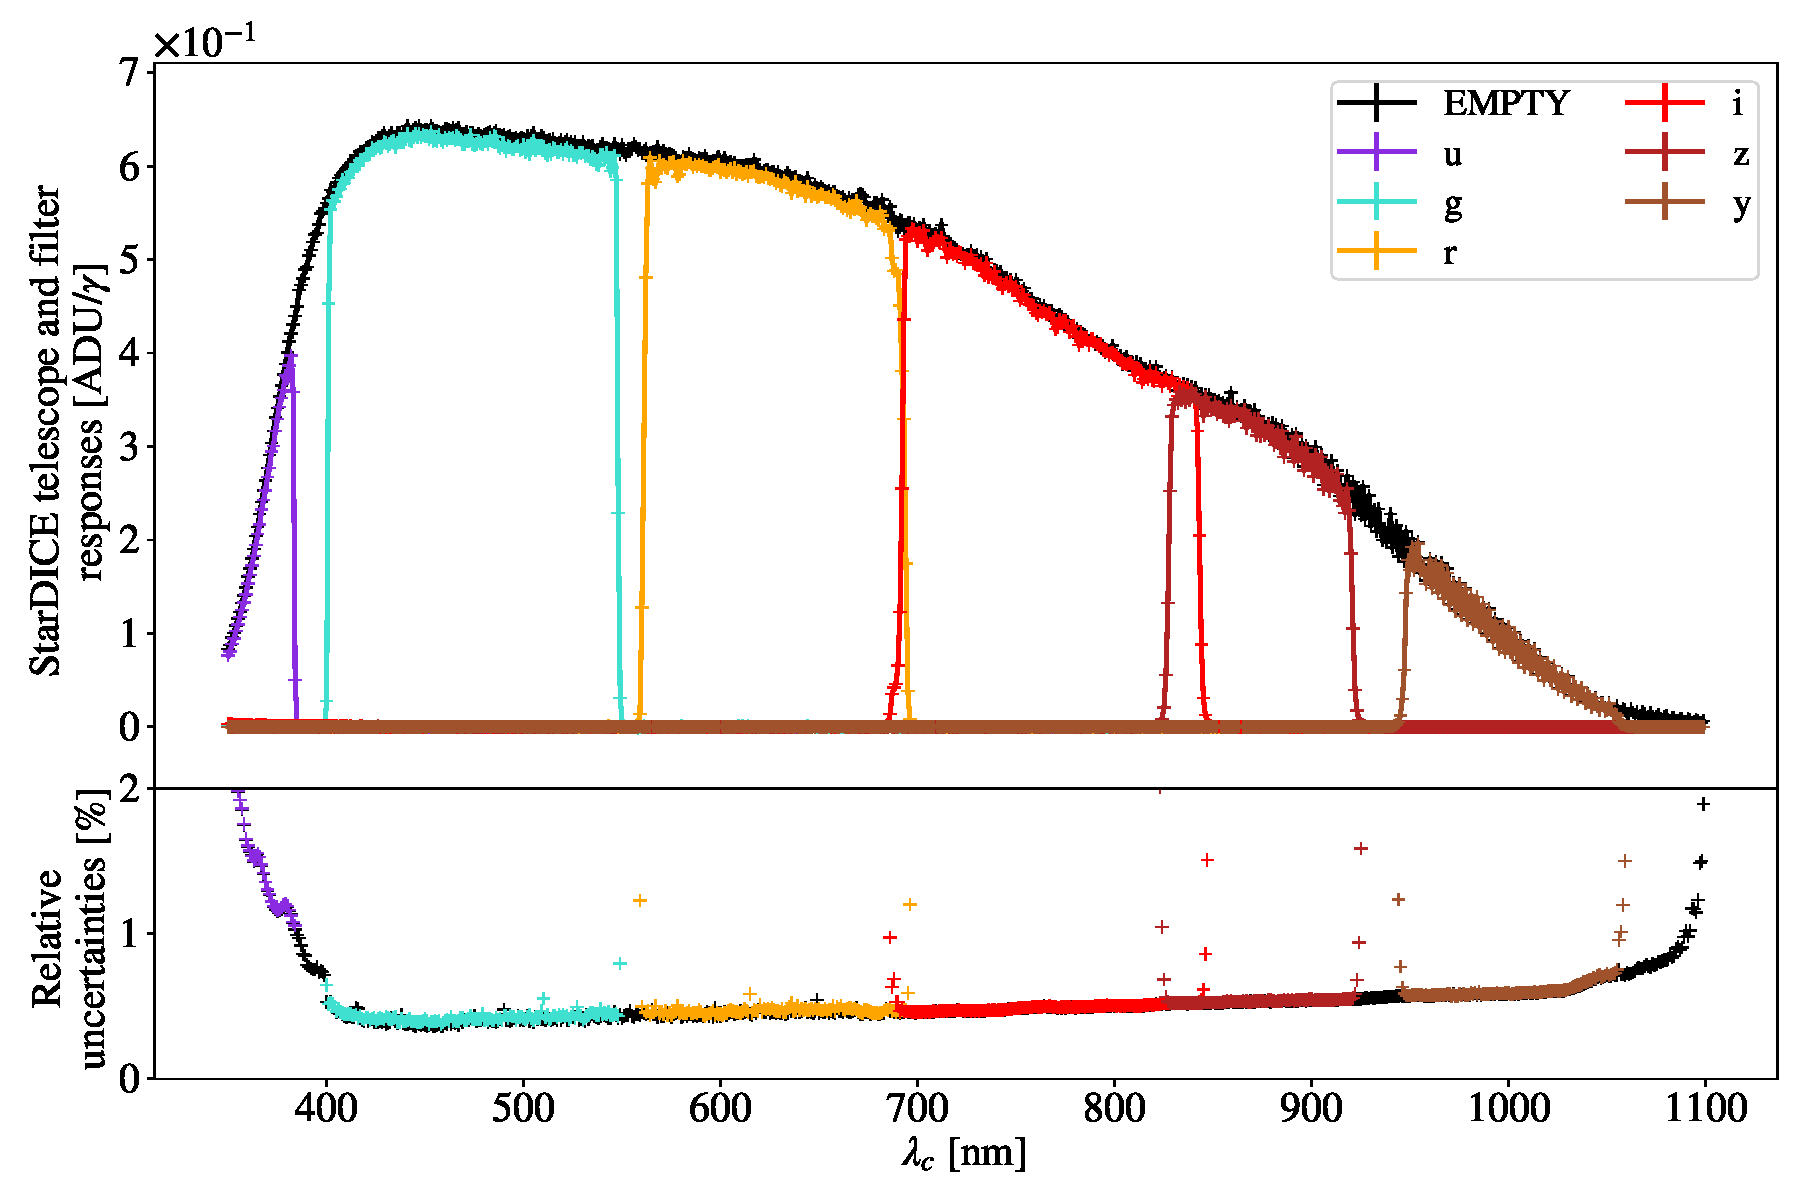
\includegraphics[width=\columnwidth]{fig/stardice_75um_response.pdf}
    \caption{Up : \SD response with at all filters and \spinhole pinhole with respect to wavelength in nanometer. \textit{Bottom:} Uncertainties over the \SD response measurement with respect to wavelength in nanometer.}
    \label{fig:stardice_75um_response}
    %~/stardice/analysis/cbp_paper/golden_sample_analysis/dr2/response_plots.ipynb
\end{figure}

\subsubsection{\SD grating transmissions}

The Figure~\ref{fig:stardice_grating_response} show the \SD response obtained with the \spinhole pinhole, with the grating set in the filterwheel. The grating being blazed so that the 1\up{st} order of diffraction is the brightest, so this is where the signal is the better as it can be seen in the relative uncertainties panel. We see a cut of the 2\up{nd} and 3\up{rd} order that correspond to the wavelength at which the signal is outside the CCD sensor.

\begin{figure}[h]
    \centering
    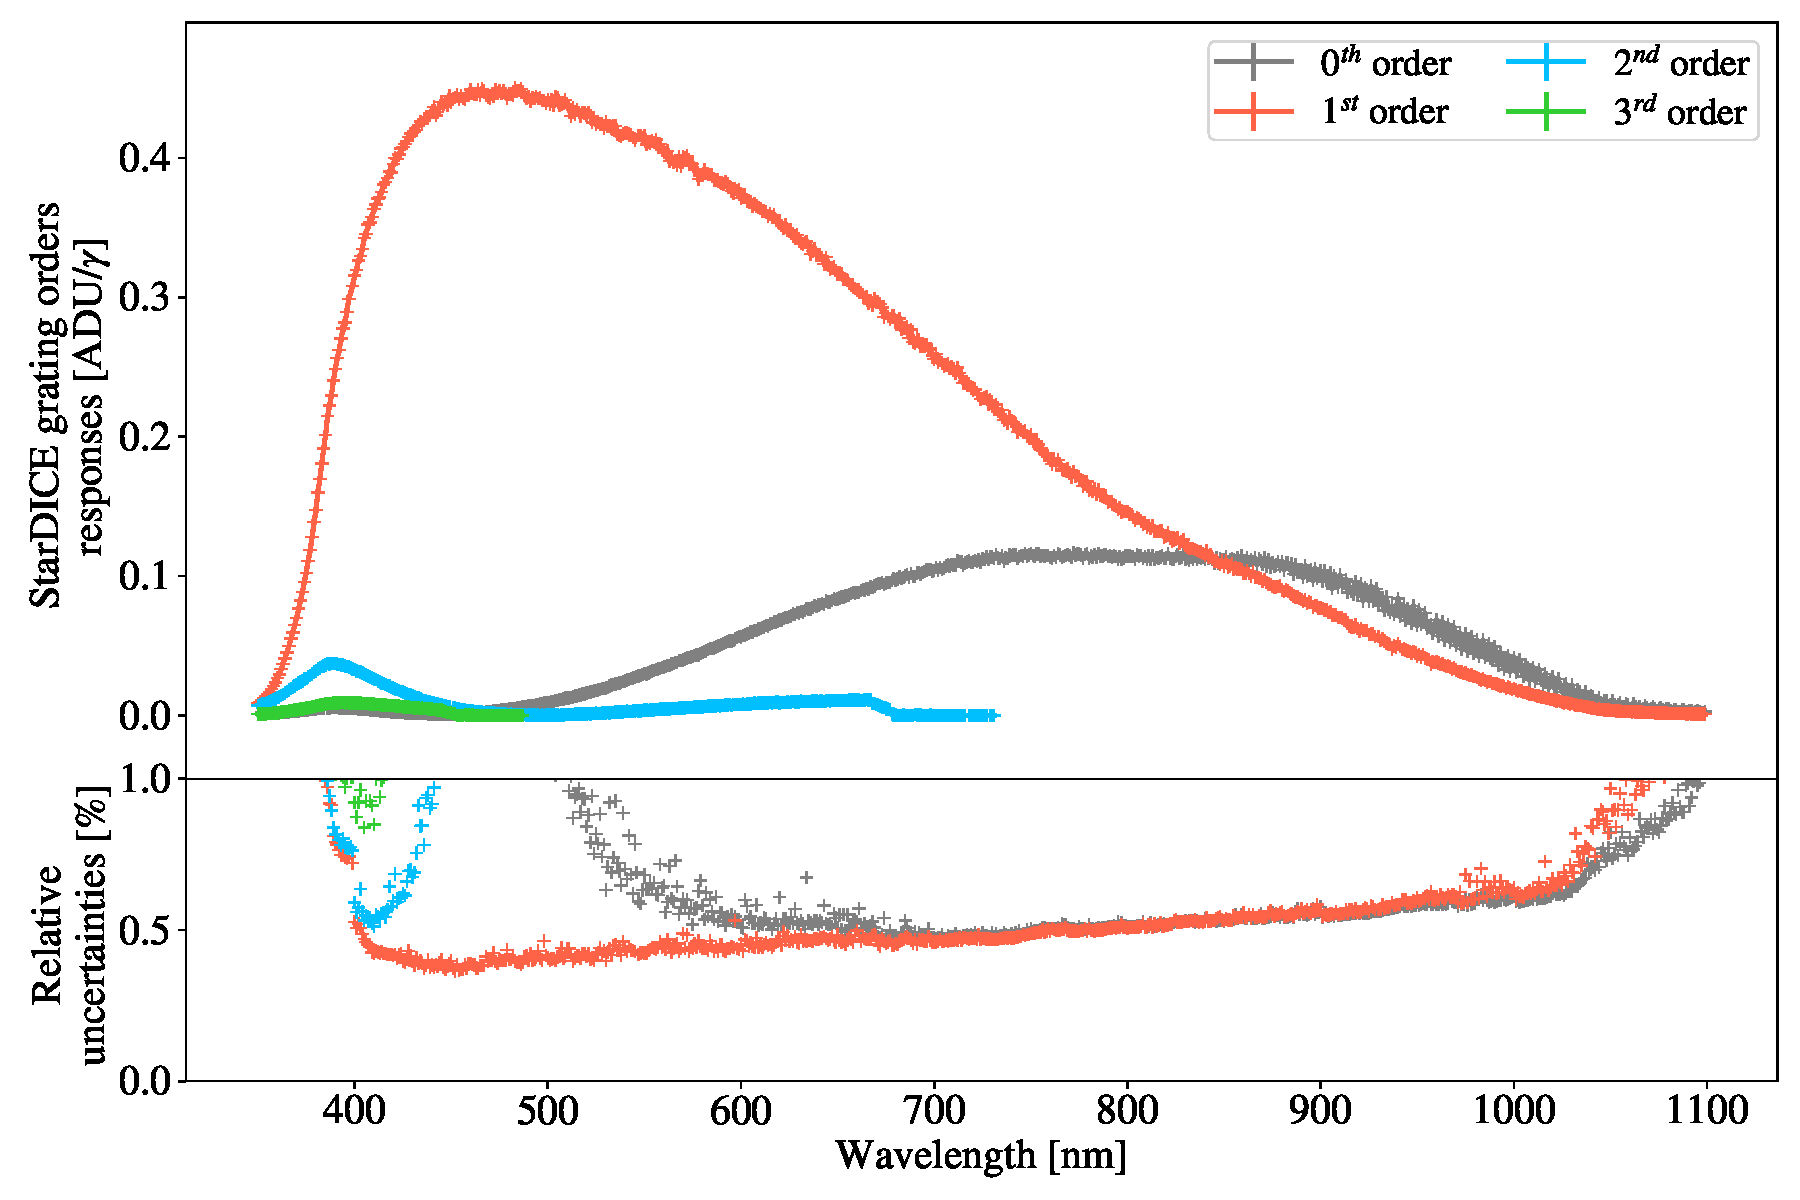
\includegraphics[width=\columnwidth]{fig/stardice_grating_response.pdf}
    \caption{\textit{Top:} \SD response with the grating in front of the camera and \spinhole pinhole with respect to wavelength in nanometer. \textit{Bottom:} Uncertainties over the \SD response measurement with respect to wavelength in nanometer.}
    \label{fig:stardice_grating_response}
    %~/stardice/analysis/cbp_paper/golden_sample_analysis/dr2/response_plots.ipynb
\end{figure}

\subsubsection{Radial positions}

The upper Figure~\ref{fig:radial_positions} show the \SD response obtained with the \spinhole pinhole and without filters for the different radial positions on the mirror shown in Figure~\ref{fig:8_mirror_positions} left, and the same focal plane position. The lower figure shows the relative difference to the mean spline going through the four responses. In the ultraviolet below \SI{450}{\nm}, we can see a significant difference between the four radial positions. It goes up to 30\%, and it will be discussed in the section \ref{sec:discussion}. What we see above \SI{1000}{\nm} in the infrared is the result of the data oscillations around the spline caused by the fringing. 

\begin{figure}[h]
    \centering
    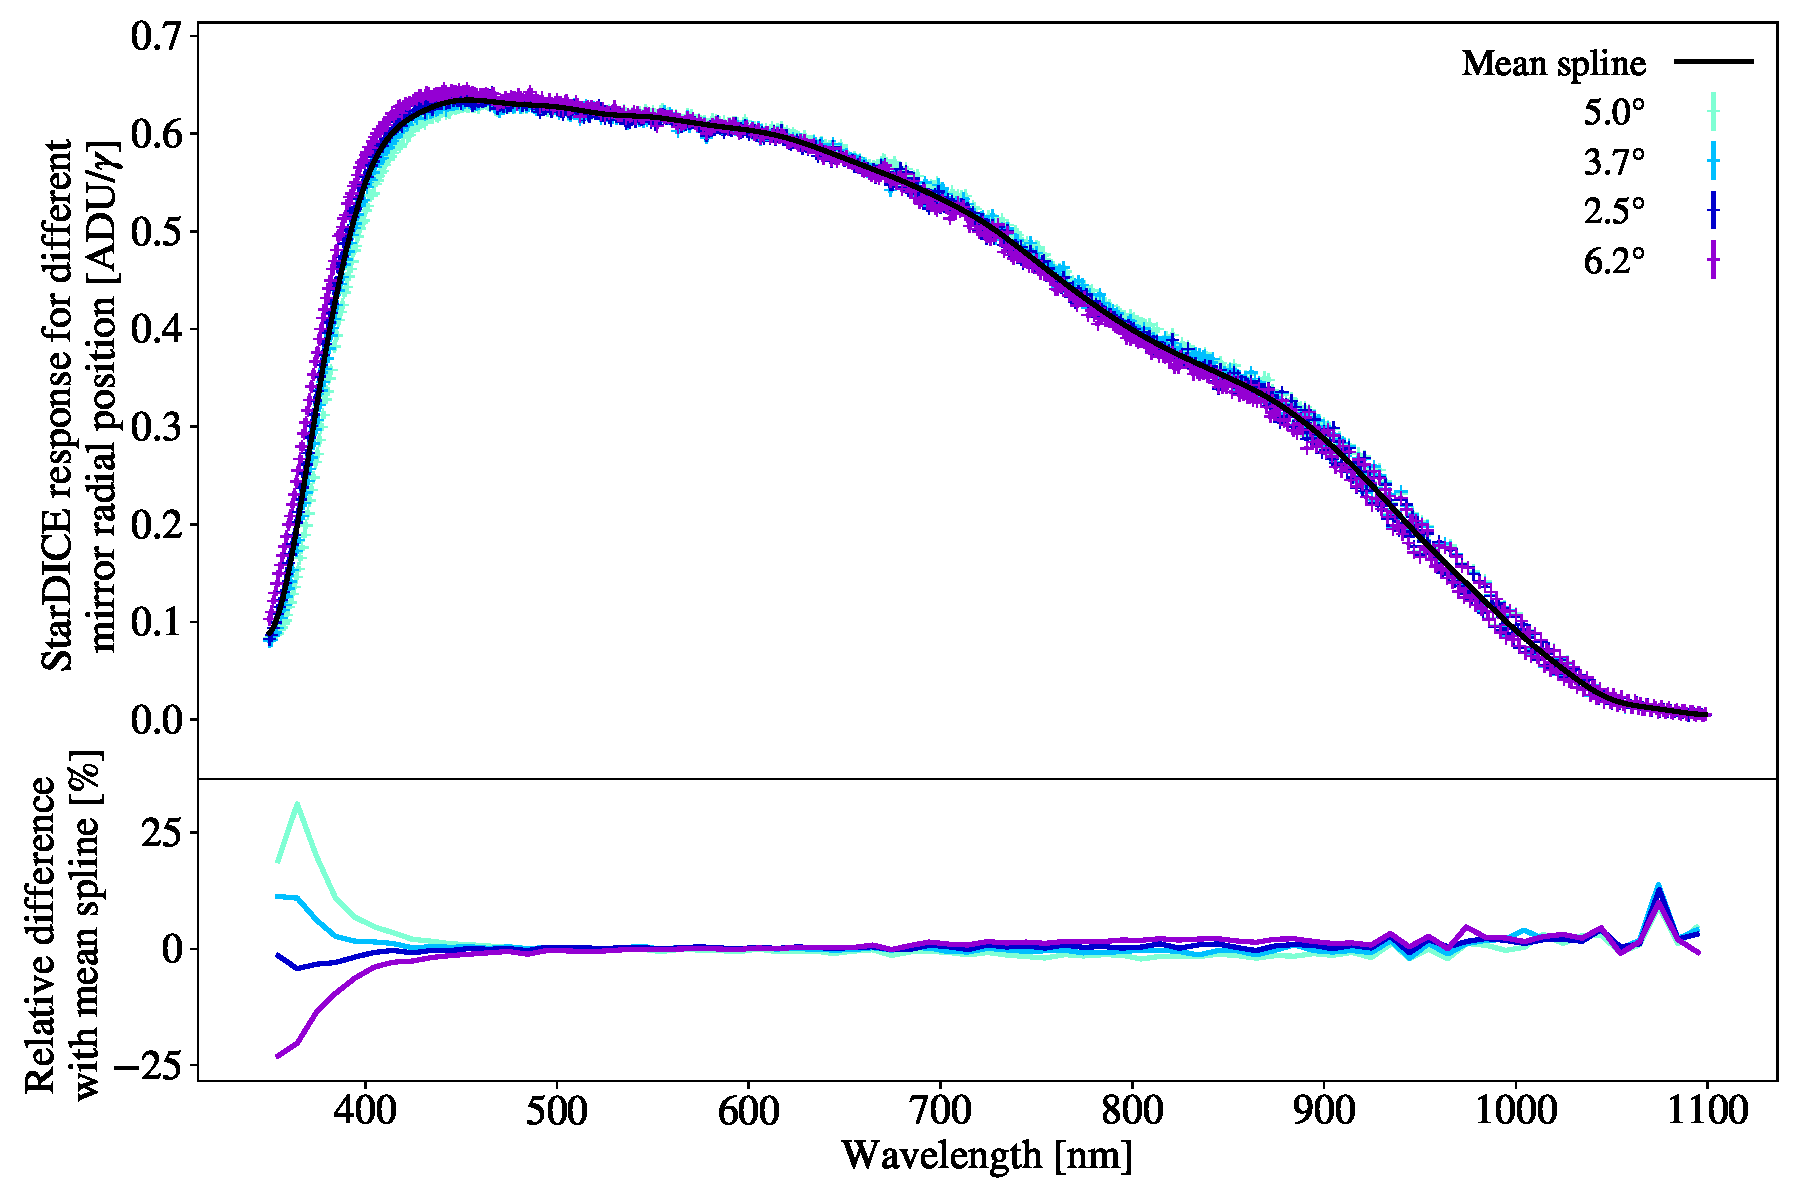
\includegraphics[width=\columnwidth]{fig/radial_positions.pdf}
    \caption{\textit{Top:} \SD response for the different radial positions on the mirror, but same position on the focal plane. \textit{Bottom:} Relative difference between the data and the mean spline.}
    \label{fig:radial_positions}
    %~/stardice/analysis/cbp_paper/golden_sample_analysis/dr2/2022_03_01_stardice_transmission_radius.ipynb
\end{figure}

\subsubsection{Quadrant positions}

The upper Figure~\ref{fig:radial_positions} show the \SD response obtained with the \spinhole pinhole and without filters for the different quadrant positions on the mirror shown in Figure~\ref{fig:8_mirror_positions} right, and the same focal plane position. The lower figure show the normalized residuals to the mean spline going through the four responses. We see again a divergence below \SI{400}{\nm} of about 20\% at most. The phenomenon in the infrared is still caused by the fringing. 

\begin{figure}[h]
    \centering
    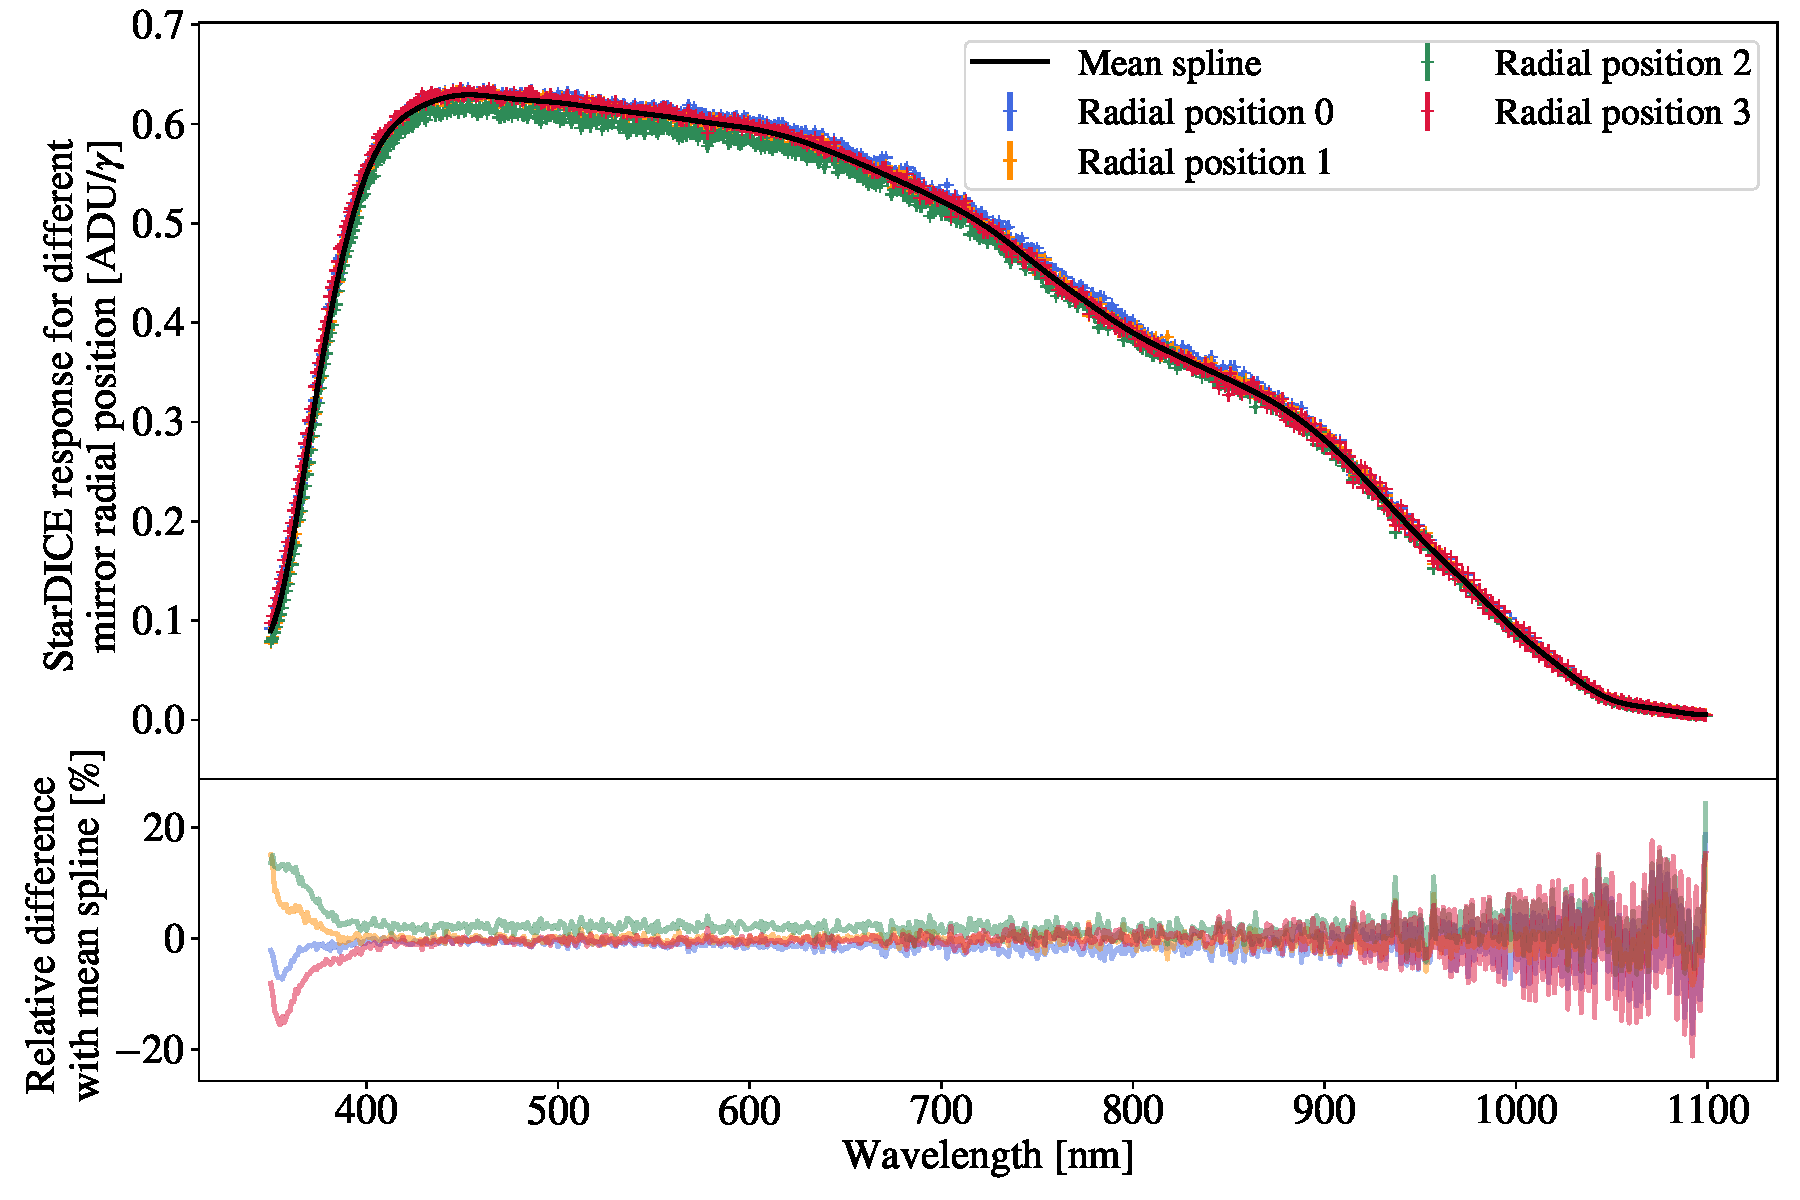
\includegraphics[width=\columnwidth]{fig/quadrant_positions.pdf}
    \caption{\textit{Top:} \SD response for the different quadrant positions on the mirror, but same position on the focal plane. \textit{Bottom:} Relative difference between the data and the mean spline.}
    \label{fig:quadrant_positions}
    %~/stardice/analysis/cbp_paper/golden_sample_analysis/dr2/2022_03_01_stardice_transmission_mirror_samples.ipynb
\end{figure}

\subsubsection{Focal plane positions}

The upper Figure~\ref{fig:ccd_positions} show the \SD response obtained with the \spinhole pinhole and without filters for the same radial and quadrant position on the mirror, and the different focal planes positions from the grid show in Figure~\ref{fig:ccd_grid}. The lower figure show the normalized residuals to the mean spline going through the sixteen responses.

\begin{figure}[h]
    \centering
    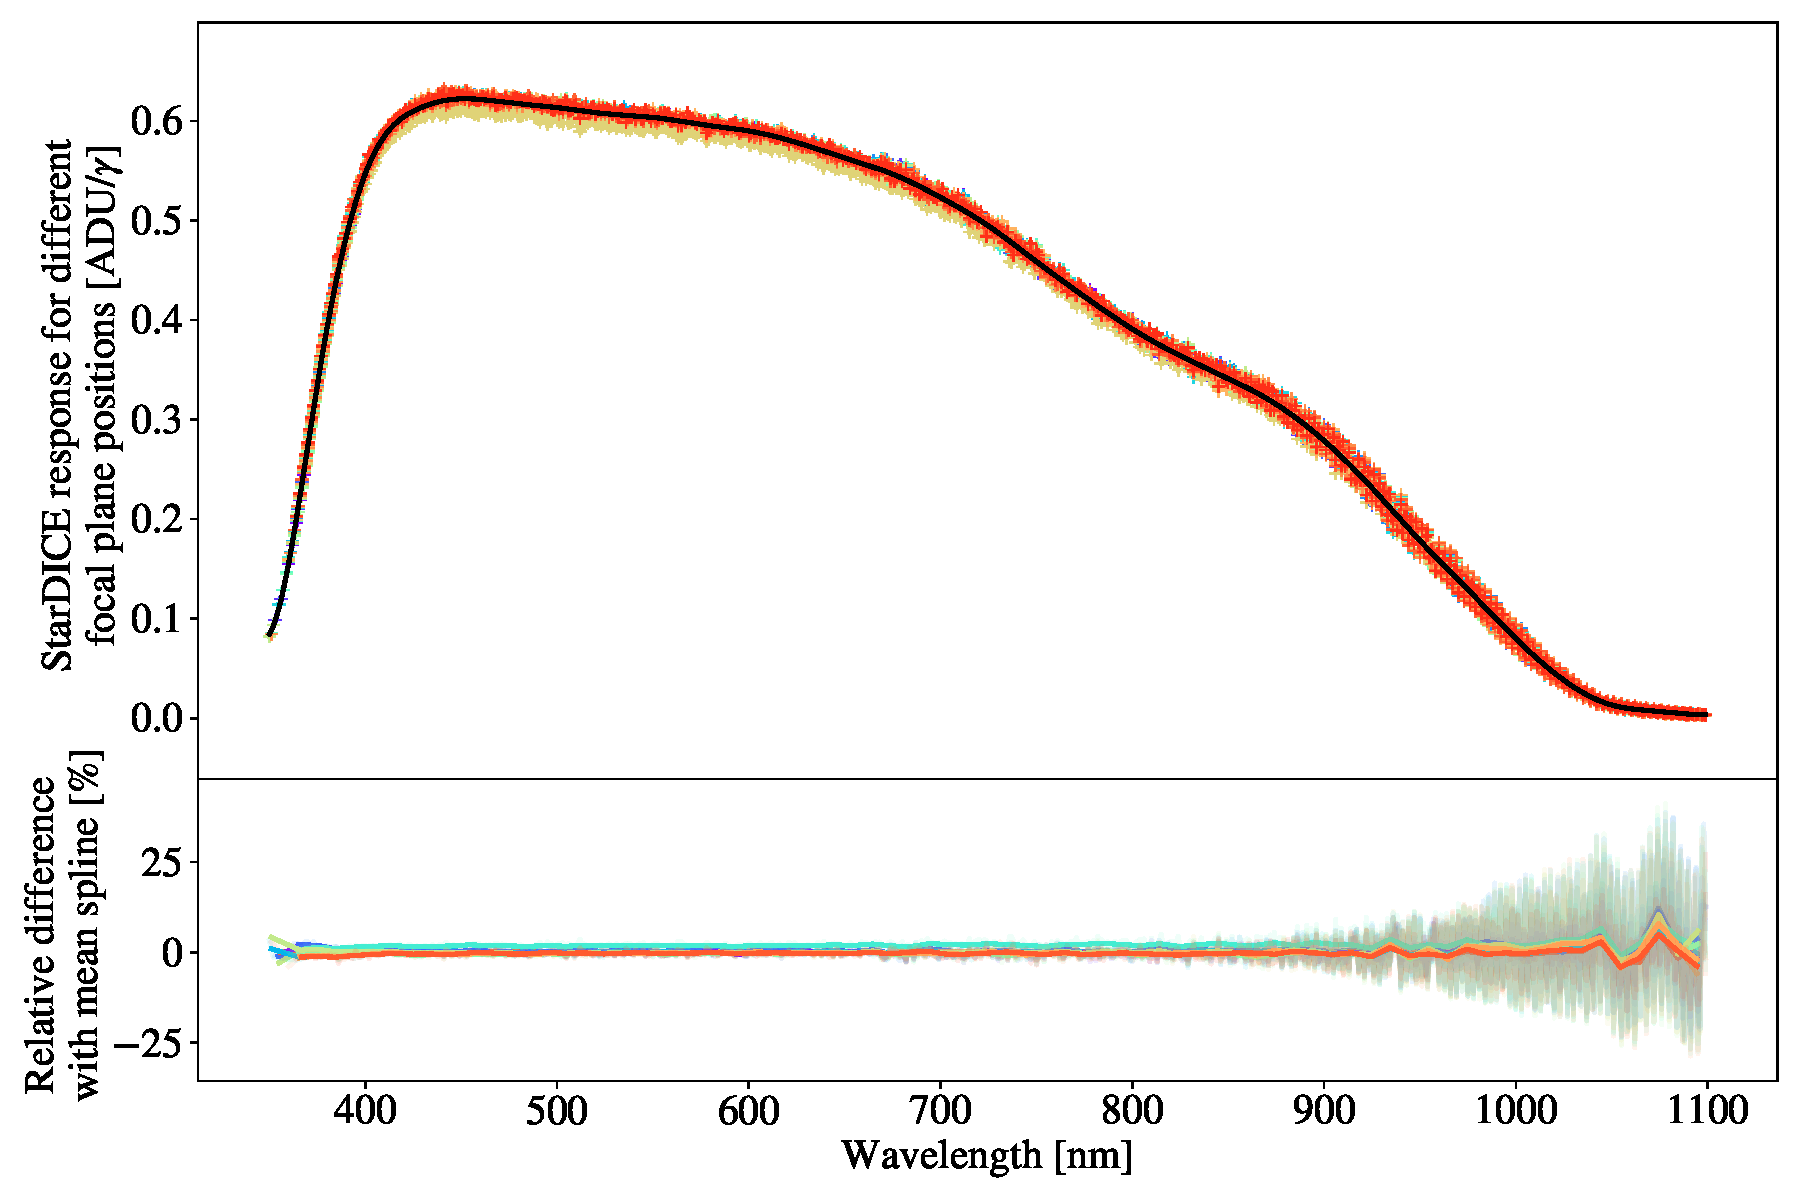
\includegraphics[width=\columnwidth]{fig/ccd_positions.pdf}
    \caption{\textit{Top:} \SD response for the different positions on the focal plane, but same position on the mirror. \textit{Bottom:} Relative difference between the data and the mean spline.}
    \label{fig:ccd_positions}
    %~/stardice/analysis/cbp_paper/golden_sample_analysis/dr2/2022_03_09_stardice_transmission_grid_auto.ipynb
\end{figure}

\subsection{Systematic uncertainties}
\label{sec:systematics}

\subsubsection{Stability of the StarDice responses}

\subsubsection{Gain and linearity}
\label{sec:gain}

Varying pinhole with StarDice, and CBP
Varying QSW but depending on result it falls into this subsection or the following

\subsubsection{Pinhole chromaticity}

\subsubsection{Pull distributions}

\subsubsection{Courbes de croissances}








\section{Synthesis of the equivalent transmission for full pupil illumination}
\label{sec:pupil_stitching}

The reflectivity of the telescope and the transmission of the filters
both exhibit a distinct radial dependency. Although the filter
transmission dependence is expected due to its interferometric nature,
the origin of the telescope reflectivity dependence remains
unclear. Despite this, we can construct an empirical model that
assumes smooth transitions between measurements and calculate the
theoretical "full pupil" transmission by averaging the model over the
illuminated portion of the primary mirror. These two steps are
necessary to achieve sub-percent color accuracy and sub-nanometer
precision in central wavelengths determination.

We also estimate statistical and systematic errors on the final
transmission curves, and propagate them through the analysis process. A
better understanding of these errors in interpreting broadband
photometry is obtained using the spectrophotometric standard star
G191B2B as a sample star.


\subsection{Radial model of the instrument transmission}
\label{sec:model}

The open transmission of the telescope is modeled as a smooth 2D
function of wavelength and incidence angle. The function is defined on
a basis of cubic B-splines, with \num{35} regularly spaced wavelength
nodes covering the range from \SIrange{350}{1100}{nm}, and two nodes
at angles corresponding to the inner and outer edges of the
occultation-free primary mirror, ranging from \SIrange{1.97}{7.24}
{\degree}. These angles represent radii of \SIrange{55}{203}{mm} for a
primary mirror with a focal length of \SI{1600}{mm}.

For data acquired using a filter, we multiply the open transmission
model by a model of the interference filter transmission, defined as
follows:
\begin{equation}
  \label{eq:filtertransmission}
T(\lambda, \theta) = \mathcal T\left(\frac{\lambda}{\sqrt{1 -
    (\sin(\theta) / n_\text{eff})^2}}\right)\,.
\end{equation}
Here, $n_\text{eff}$ is an effective index for the filter,
and T is a piece-wise linear function of wavelength. The piece-wise
linear function is initially created with \num{150} regularly spaced
nodes between \SIrange{350}{1100}{nm}, providing a general resolution
of \SI{5}{nm}. In cases where more precision is needed, we further
refine the grid by equally splitting intervals where the local mean
chi-square exceeds the global mean chi-square by more than three
standard deviations. This process is repeated four times to ensure
that filter fronts are typically modeled with up to approximately
\SI{0.3}{nm} resolution.


In the specific case of the  grating zeroth and first orders, the photometry is
adjusted using a cubic B-spline model with \num{105} nodes in
wavelength.

The composite model is fit to dataset No.~2, which includes data
from four different radii and successive observations without filters
or with all seven filters and the grating. The baseline model has
\num{1979} free parameters: \num{148} for the open transmission,
approximately $6\times165$ for each of the $ugrizy$ filters, and
\num{420} for each of the grating orders. Unfortunately, the blue edge
of the $u$-band filter cannot be accurately measured with this
data. Fit results are displayed in
Fig.~\ref{fig:lambdathetafitresults}.

\begin{figure*}
  \centering
  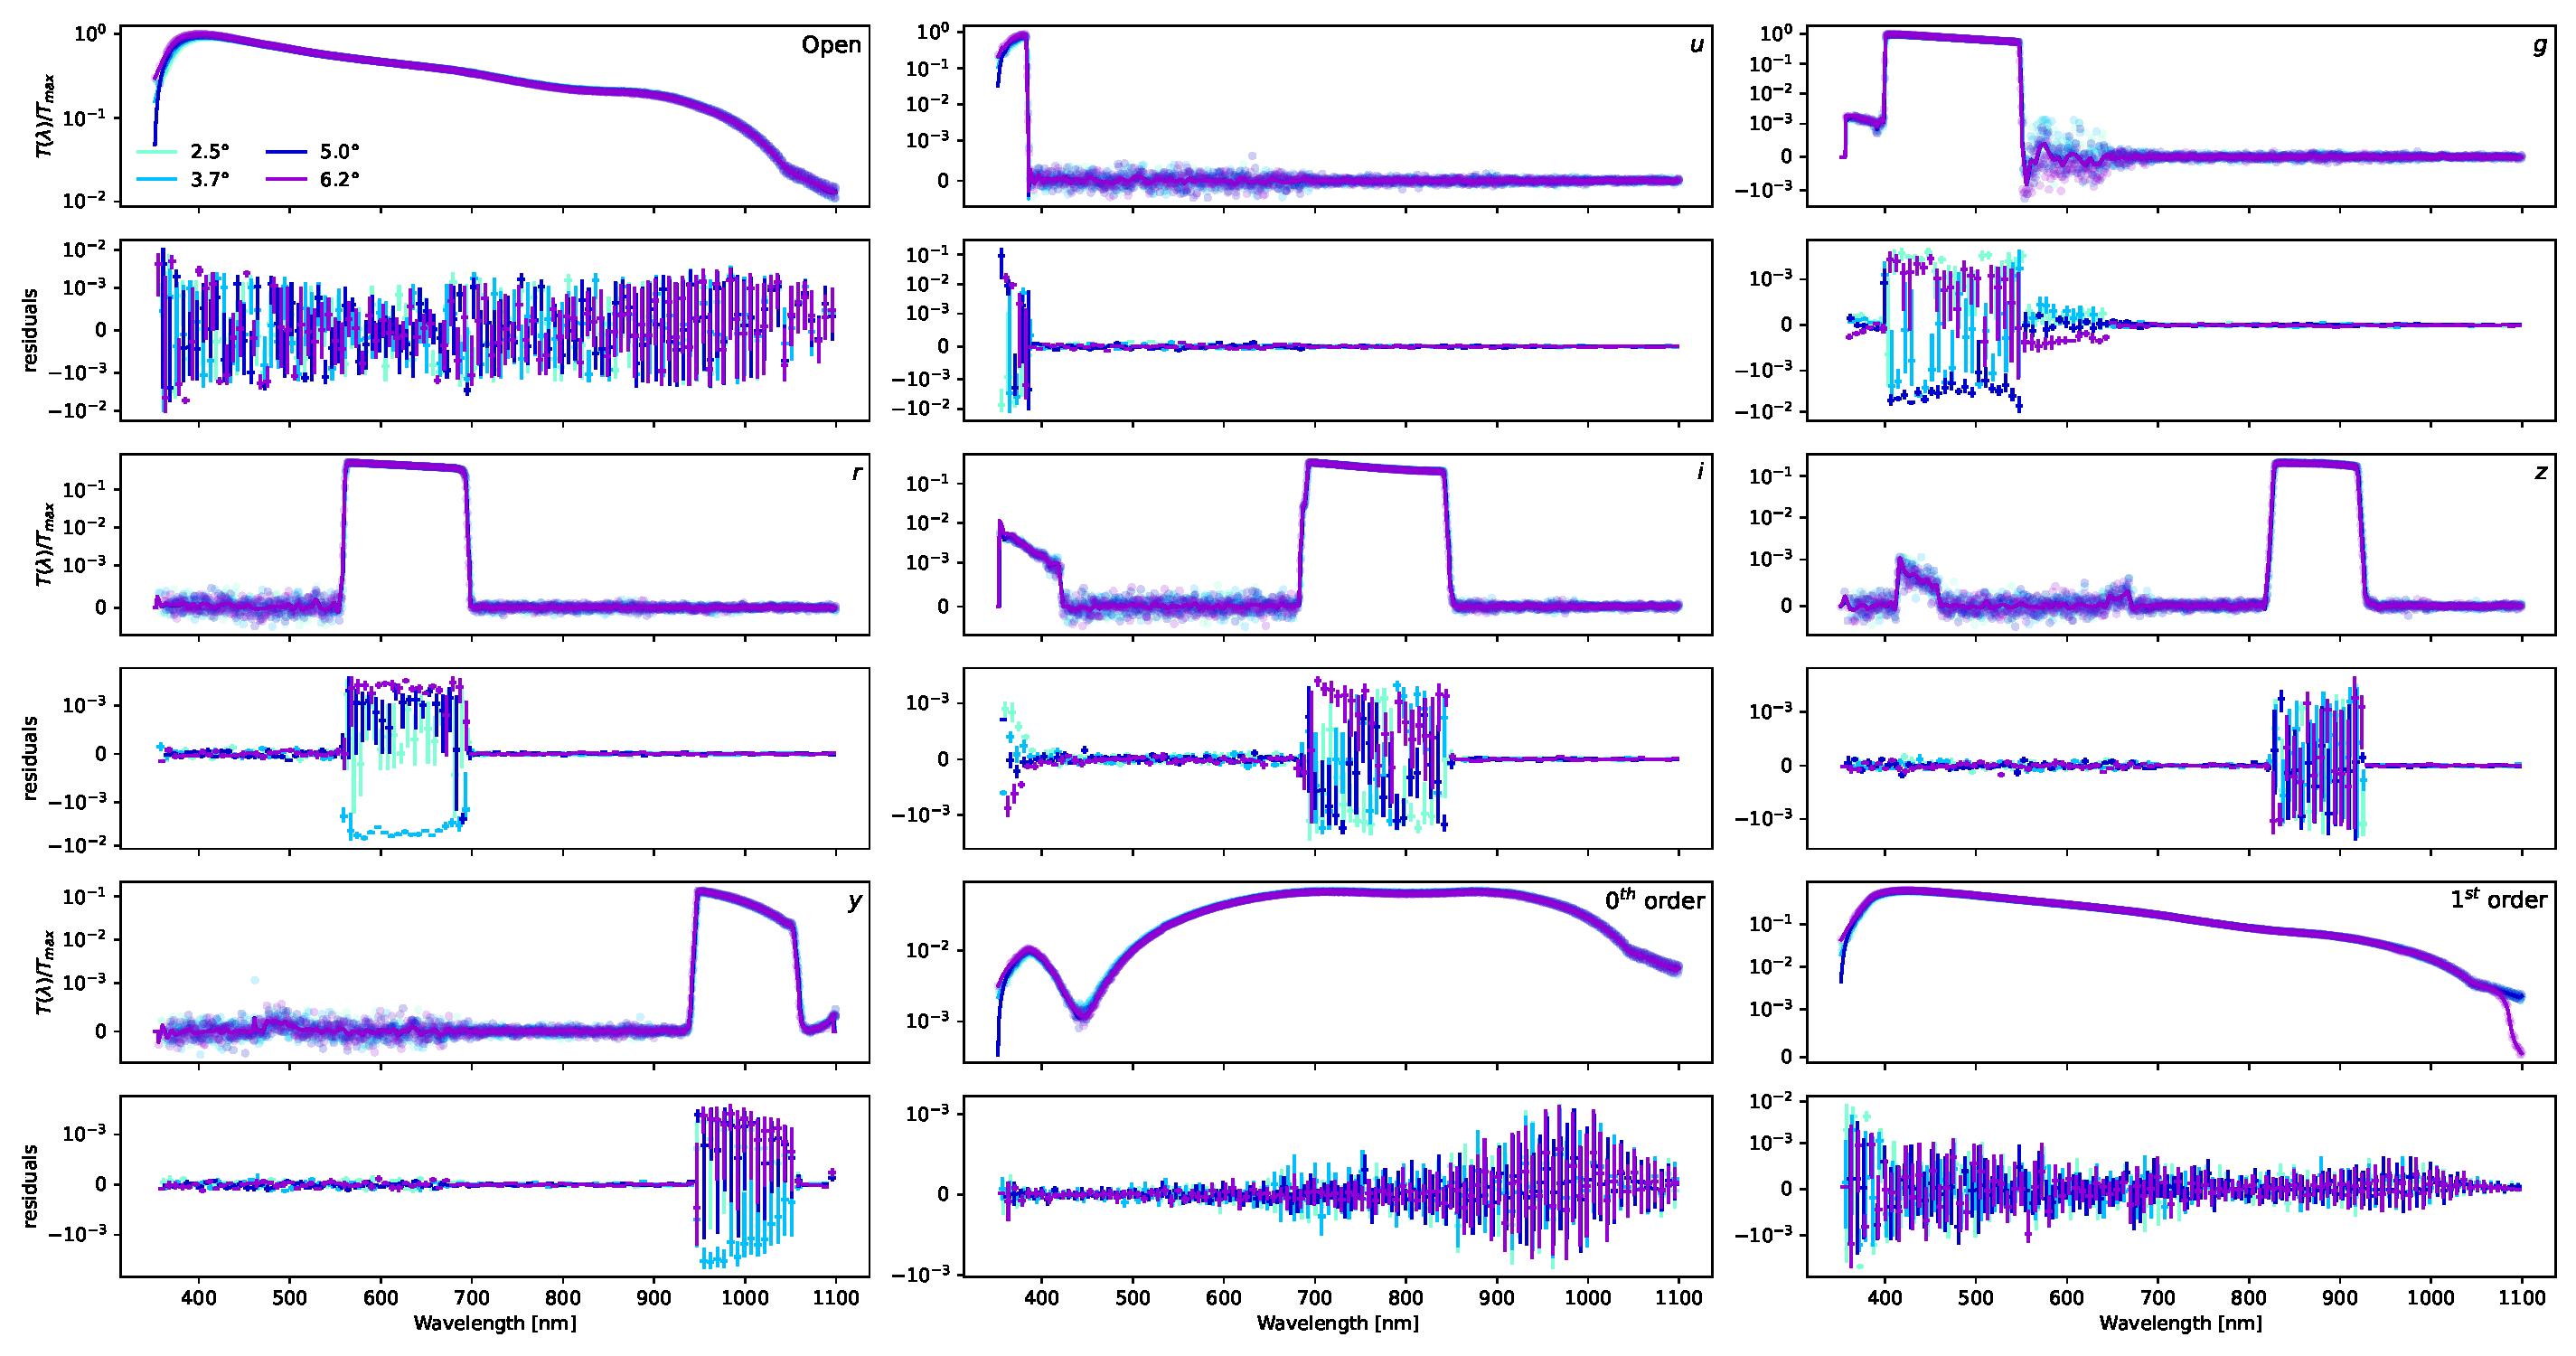
\includegraphics[width=1\linewidth]{./fig/lambdathetafitresults.pdf}
  \caption{Model of the wavelength and radial dependency of the
    StarDICE response to CBP illumination $R(\lambda)$. Each panel
    display the raw measurements at the 4 sampled position for each of
    the filter configurations: no filters (Open), with one of the 6
    photometric filters ($ugrizy$) or with the grating looking either
    at the zeroth order or the first order spots. The panel
    immediately below each panel display the residuals to the
    model. For easy comparison, all panels are normalized to the peak
    of the response, which occurs in the open configuration at
    $\lambda = \SI{398}{nm}$ and $\theta = \SI{6.2}{\degree}$.
    %\textbf{SZF: les résidus de l'open transmission sont sur une échelle différente des autres}
 }
  \label{fig:lambdathetafitresults}
\end{figure*}


\begin{figure}
  \centering
  \includegraphics[width=1\linewidth]{fig/diffraction_dust.png}
  \caption{Diffraction rings due to the presence of a dust spot on the
    r filter, intercepting the CBP beam. Red circles are over-plotted
    to ease the visualisation.}
  \label{fig:dust}
\end{figure}


Overall, the model provides a satisfactory description of the
dataset. The most significant discrepancy is a noticeable gray
decrease of the transmission of the $r$ filters for the sample
measurement at \SI{3.7}{\degree} with respect to the average of the
other three.  After investigating this issue, we identified that the
corresponding images displayed a diffraction figure consistent with
the presence of a dust particle on the filter surface intercepting the
CBP beam.  Based on the approximate area of the beam spot
($\sim$\SI{12}{\milli\metre\squared}), and the estimated particle size range (between
\SIrange{200}{300}{\micro\metre}), we calculated a potential decrease
in transmission for this specific partial illumination of the primary
mirror of up to \SI{0.6}{\percent}. This value is in good agreement
with the observed decrease. Similar discrepancies were found for some
observations in $u$, $g$ and $y$ bands, although determining particle
sizes from diffraction features was not possible in these cases. We
attribute these discrepancies to dust contamination on the filter
surface as well.

The top panel of Fig.~\ref{fig:metrics} shows the difference between
the transmission integral for measurements and the model at each
position, helping readers better visualize the 'gray'
discrepancies. The standard deviation of model/measurement
discrepancies is \SI{10.2}{mmag}. Considering this value as an
estimate of dust-induced dispersion, we can deduce that the
corresponding uncertainty for per-filter normalization of the model
(averaging 4 independent samples) is approximately $\SI{5}{mmag}$.

This noise could be decreased by averaging more sample measurements of
the mirror. In our case 4 additionnal positions were sampled as part
of run 3 (see table~\ref{tab:schedule}). However, while run 2
measurements were carefully taken to sample the mirror from the outer
edge to the inner edge along a radius with separations provided by the
mount encoders, the other measurements were positioned semi-randomly
with the idea that the position of the CCD-window ghost in the images
will enable precise determination of the position of the beam in the
mirror. Two issues were overlooked at this stage which complicate the
determination of the geometry from the position of the ghosts: (1) The
wedge of the CCD window and (2) the ghost positions dependence on the
conjugation relation between the CBP and the telescope which is only
approximately known. The complexity of including those parameters in a
full model of the telescope+CBP sets the analysis of those data out of
the scope of the current paper.

The bottom panel in Fig.~\ref{fig:metrics} displays the difference
between the measured central wavelength and the model-predicted value
for all 4 radius positions. The model accurately reproduces the
central wavelengths of all filters with a standard deviation of only
$\SI{0.13}{nm}$. This represents an improvement by an order of
magnitude compared to a model that neglects wavelength shift
considerations, highlighting the importance of including this effect
in the StarDICE response model.

\begin{figure}
  \centering
  \includegraphics[width=1\linewidth]{fig/metrics.pdf}
  \caption{Discrepancies between model and raw measurements at
    different mirror locations summarized according to 2 metrics:
    \emph{Top:} relative difference in the integral of the passband,
    expressed in millimagnitudes; \emph{Bottom:} relative difference
    in central wavelength computed as the barycenter of the passband.}
  \label{fig:metrics}
\end{figure}

\subsection{Full pupil synthetic transmission curves}

The full pupil transmission is synthesized by numerically averaging
the above model assuming that the pupil is a perfect annulus with an
inner radius of \SI{55}{mm} and an outer radius of \SI{203}{mm},
corresponding to an effective mirror area of \SI{1202}{cm^2}. A
rectangular quadrature with 100 evenly sampled points in radius has
been used for the averaging. The curves have been normalized using the
CBP response from Sect.\ref{sec:cbp}. The resulting transmission
curves are shown in Fig.~\ref{fig:fullpupiltrans}.
\begin{figure}
  \centering
  \includegraphics[width=1\linewidth]{fig/fullpupill.pdf}
  \caption{Full-pupil transmission curves for the StarDICE instruments.}
  \label{fig:fullpupiltrans}
\end{figure}


\subsection{Final uncertainty budget}

The impact of the uncertainties in our determination of the full-pupil
transmission curves depend on the application. We first consider the
use of the CBP as the sole source for absolute calibration of the
instrument response and then its use in conjonction with a broadband
star-like calibration light-source.

\subsubsection{Uncertainties in absolute fluxes}
\label{sec:absolute}

The first obvious application is to take
each curve as an absolute calibration of the instrument throughput and
use it to interpret broadband fluxes measured by this instrument,
according to the equation:
\begin{equation}
  \label{eq:mb}
  \phi_b = \int_\lambda  R_b(\lambda) A(\lambda) S(\lambda) \lambda d\lambda
\end{equation}
where $R_b$ is the full pupil response curve of the instrument
synthesized previously, $S$ is the top of the atmosphere spectrum of
the target and $A$ is the atmospheric transmission for this
observation. Setting aside the question of the atmospheric
transmission, the error $\delta R_b$ on the passband will translate
into an error on the synthesized flux $\delta \phi$, whose magnitude
depends on the spectrum of the object. As an illustration we
propagated all our uncertainties to the synthetic fluxes of the
primary spectrophotometric standards G191B2B. We report the results in
Table~\ref{tab:budget} as the relative uncertainty on the broadband
flux $\sigma(\delta \phi)/\phi$ for each band, with one line per
contributions. The table does not include the uncertainty on the gray
scale, mainly coming from the uncertainty in the effective area of the
telescope which cannot be determined accurately with such a setup. 

% Pas de gray scale
\begin{table}
  \centering
  \caption{Relative uncertainty in the synthetic broadband fluxes of
    G191B2B, split by contributions, in permil.}
  \label{tab:budget}
  \begin{tabular}{@{}l@{}rrrrrr@{}}
    \toprule
    \toprule
    Source & $u^\dag$ & $g$ & $r$ & $i$ & $z$ & $y$ \\
    & $[\text{\textperthousand}]$ & $[\text{\textperthousand}]$ & $[\text{\textperthousand}]$ & $[\text{\textperthousand}]$ & $[\text{\textperthousand}]$ & $[\text{\textperthousand}]$\\
    \midrule
    StarDICE & 0.5 & 0.2 & 0.2 & 0.3 & 1.0 & 3.8 \\
    $\eta_{SC}$ & 1.6 & 0.1 & 0.1 & 0.1 & 0.1 & 0.1 \\
    CBP & 2.2 & 0.5 & 1.2 & 0.0 & 0.0 & 0.1 \\
    \midrule
    Stat (total) & 2.7 & 0.5 & 1.2 & 0.3 & 1.0 & 3.8 \\
    \midrule
    Scattered light & 2.7 & 3.1 & 3.8 & 4.3 & 4.8 & 5.3 \\
    Repeatability & 0.8 & 0.4 & 0.5 & 1.1 & 1.1 & 1.1 \\
    Linearity & 0.2 & 0.2 & 0.3 & 0.5 & 0.5 & 0.5 \\
    Contamination & 4.4 & 0.6 & 0.8 & 0.1 & 0.1 & 0.1 \\
    Mirror sampling noise & 5.4 & 5.4 & 5.4 & 5.4 & 5.4 & 5.4 \\
    NIST photodiode & 0.2 & 0.1 & 0.0 & 0.0 & 0.0 & 0.1 \\
    Solar Cell temperature & 0.0 & 0.0 & 0.0 & 0.0 & 0.0 & 3.9 \\
    wl cal & 0.7 & 0.6 & 0.5 & 0.4 & 0.3 & 0.3 \\
    \midrule
    Syst (total) & 7.6 & 6.3 & 6.7 & 7.1 & 7.4 & 8.7 \\
    \midrule
    Total & 8.0 & 6.3 & 6.8 & 7.1 & 7.5 & 9.4 \\
    \bottomrule
  \end{tabular}
  \tablefoot{$^\dag$Our measurement does not capture the blue side of the $u$ band filter. We propagate uncertainties as if the transmission was dropping to 0 at the edge of the measurement to illustrate the performances that would be obtained from a complete measurement. For all practical purposes however, the actual $u$ band transmission cannot be determined from the existing measures.}
\end{table}

The dominant contributor to the uncertainty in our flux reconstruction
is the mirror sampling noise. With the CBP beam sampling only a small
fraction of the primary mirror, and therefore a small fraction of the
filters, any inhomogeneity in the transmission of the filter ends up
causing a noise in the band to band ratio of transmissions. This noise
decreases with more sampling points on the primary mirrors, at a large
observational cost.

The next significant issue is the difficulty to get rid of
non-collimated (scattered) light during the calibration of the CBP on
the solar-cell array. A natural way to deal with this issue would be
to significantly increase the solar-cell CBP distance. In our case
however the beam created by the \bpinhole pinhole already barely fit
inside the footprint of the solar cell. Increasing the solar-cell CBP
distance would have caused issues for the collimated beam calibration in exchange
for getting rid of the non-collimated light.

Some caution needs to be payed to changes in the working temperature
of photodiodes when calibrating $y$ band. In our current measurement,
the uncertainty in the difference in temperature between the
calibration of the solar-cell and its use to calibrate the CBP is
quite large (\SI{1.6}{\celsius}). This has easily been fixed in latter
iteration of the solar-cell design by including temperature sensors
directly cell enclosure.

Our mitigation procedure for the contamination of the beam by light
at different wavelengths is found satisfactory for all bands but $u$. This
is due to the remaining uncertainties in the determination of the
phosphorescence contribution in the integrating sphere.

\begin{figure}
  \centering
  \includegraphics[width=1\linewidth]{fig/bandcorrelation.pdf}
  \caption{Correlation of the uncertainties on the synthetic fluxes of G191B2B.}
  \label{fig:correlation}
\end{figure}

Lastly, most systematic uncertainties have modes coherent across
wavelengths. As a result, the errors induced on broadband magnitudes
are correlated across bands, with typical correlation levels in the
20-40\% range. The correlation matrix resulting from the full
propagation of uncertainties identified in Table~\ref{tab:budget} is
displayed in Fig.~\ref{fig:correlation}. Again, we do not account for
the uncertainty in the gray scale which is perfectly correlated
between all bands and would dominate the uncertainty budget.

\subsubsection{Uncertainties in relative fluxes}
\label{sec:relative}

The more common application of telescope transmission measurements is
to rely on the transmission curves to predict actual
observations of a spectrophotometric standard of known flux and
determine an independent re-calibration factor for each band. The
errors on the interpretation of observations of another object will
then depend on the difference in color between the object and the
spectrophotometric standard, canceling for objects whose spectrum is
very similar to the spectrum of the standard.

For the StarDICE telescope, the role of photometric standard is played
by a collection of narrow-spectrum LEDs, whose observations set the
absolute normalization of each bands. The telescope is then used to
follow CALSPEC standard stars and precisely measure their broadband
fluxes. In this operation, all uncertainties which mostly impact the
normalisation of the passbands cancel out. In order to illustrate the
impact of the uncertainties in our passband determination in this
case, we modeled the spectrum of 6 calibration LEDs as Gaussian shapes
centered on the central wavelength of each filter with a full-width
half-max of 7\% in wavelength. 
To simulate the effect of the passband recalibration on LED
observations, we propagate the uncertainties on the \emph{ratios} of
broadband fluxes between the LEDs and G191B2B. The results are
presented in Table \ref{tab:led}. As expected, most broadband error
sources cancel out, resulting in an accuracy of the order of 1 permil,
matching the requirements for the StarDICE experiment.

In contrast, the sensitivity to wavelength calibration generally
increase in a way that depends on the spectra of the LEDs. The flux of
LEDs whose spectrum overlap with the edges of the filters are more
strongly affected by wavelength calibration errors than LEDs whose
spectrum is largely contained in the filter passband. The design of
the StarDICE artificial star include both cases, with the idea that
overlapping LEDs can provide a handle to test (or correct) for filter
front errors. Here we report sensitivity for non-overlapping LEDs
assuming no specific correction.

\begin{table}
  \centering
  \caption{Uncertainties in the flux of G191B2B after recalibration by observation of narrow-spectrum LEDs centered on the filter passband.}
  \label{tab:led}
  \begin{tabular}{@{}l@{}rrrrrr@{}}
    \toprule
    Source & u & g & r & i & z & y \\
           & $[\text{\textperthousand}]$ & $[\text{\textperthousand}]$ & $[\text{\textperthousand}]$ & $[\text{\textperthousand}]$ & $[\text{\textperthousand}]$ & $[\text{\textperthousand}]$\\
    \midrule
    StarDICE & 0.2 & 0.3 & 0.2 & 0.2 & 0.5 & 1.8 \\
    $\eta_{SC}$ & 0.4 & 0.1 & 0.1 & 0.1 & 0.0 & 0.1 \\
    CBP & 0.5 & 0.5 & 1.1 & 0.0 & 0.0 & 0.0 \\
    \midrule
    Stat (total) & 0.7 & 0.6 & 1.1 & 0.2 & 0.5 & 1.8 \\
    \midrule
    Scattered light & 0.0 & 0.1 & 0.0 & 0.0 & 0.0 & 0.0 \\
    Repeatability & 0.0 & 0.0 & 0.1 & 0.0 & 0.0 & 0.0 \\
    Linearity & 0.0 & 0.0 & 0.0 & 0.0 & 0.0 & 0.0 \\
    Contamination & 0.1 & 0.1 & 0.0 & 0.0 & 0.0 & 0.0 \\
    Mirror sampling noise & 0.0 & 0.0 & 0.0 & 0.0 & 0.0 & 0.0 \\
    NIST photodiode & 0.1 & 0.1 & 0.0 & 0.0 & 0.0 & 0.1 \\
    Solar Cell temperature & 0.0 & 0.0 & 0.0 & 0.0 & 0.0 & 0.6 \\
    wl cal$^\dag$ & 0.3 & 0.5 & 0.6 & 1.1 & 0.9 & 1.4 \\
    \midrule
    Syst (total) & 0.3 & 0.5 & 0.6 & 1.1 & 0.9 & 1.5 \\
    \midrule
    Total & 0.8 & 0.8 & 1.3 & 1.1 & 1.1 & 2.4 \\
    \bottomrule
  \end{tabular}
  \tablefoot{$^\dag$The impact of wavelength calibration on
    led-calibrated fluxes depends significantly on the exact spectrum
    of the LEDs. The numbers presented comes from simulation of a
    realistic case, but the numbers for actual LEDs may differ.}
  
\end{table}




\section{Conclusion}
\label{sec:discussion}

We determined the response of the 16'' StarDICE telescope using a
collimated beam projector (CBP) powered by a tunable laser. Our
procedure involved three main steps. In a first step we measured the
throughput of the CBP with a wavelength sampling of \SI{1}{nm} between
350 and \SI{1100}{nm} by illuminating a calibrated solar cell. We then
used the calibrated beam to map the response of the StarDICE telescope
at all wavelengths and at several positions on its primary
mirror. Lastly, we interpolated between the sample points to
synthesize the equivalent response of the telescope to illumination
of its full pupill.

A key aspect in the process of calibrating the CBP beam is that the
sensitive area of the photodiode is large enough to cover entirely the
beam. While the measurement is simple in its principle, special
care must be given to several aspects of the setup and analysis to
reach the required level of accuracy. Most notably: (1) the laser beam must be filtered to improve the purity of its wavelength
composition, even with the mitigation measures we adopted, unavoidable
contamination had to be subtracted in the analysis; (2) the setup must minimize scattered light which affects differently the calibration solar cell and the calibrated telescope; (3) achieving sufficient signal to noise ratio in the solar cell implies to fight with high level of pink noise.

To deal with this issue, we selected a solar cell with high
impedance, and grouped the light deposit in short bursts to reduce the
pink noise effects while illuminating the solar cell.
These bursts were separated by dark periods. Using a good synchronization in time
between the bursts and the photocurrent measurements, 
we could estimate the dark current contribution and correct it.
Additionnaly, we increased the collected flux in the solar cell 
by selecting a larger pinhole, inducing a small but measurable change in the
chromatic throughput of the CBP, which must be accounted for.
We did not found significant non-linearities in our measurement
chain. Repeating the measurements allowed to identify slight
evolution in the throughput which were easily corrected

Most of the measurement time is spent in mapping the telescope
response which scales linearly with the number of filters,
resolution in wavelength and number of mirror samples taken. Our main
4-positions survey which yields subpercent precision on the
synthesized passbands involved about 30000 images. The complete
dataset, including runs for the characterization of systematics,
pinhole intercalibration and focal plane survey, is closer to 200000
images. With our fully automated setup, collecting this dataset required
7 days of uninterrupted operation. 

The survey allowed to determine filter fronts with a precision of
about \SI{0.2}{\nano\meter}, to accurately measure out-of-band leaks at a relative
level of \num{e-3} and revealed an unexpected and strong dependency of
the mirror reflectivity with the incidence angle in the UV. As a
result we were able to show through simulations that the uncertainties in our determination of the
telescope passbands will not contribute more than 1\textperthousand\
uncertainty in the measurement of broadband flux with StarDICE after
calibration by observations of the artificial star. 

The results presented in this paper also serve as a proof of concept for the Rubin CBP, specifically designed for measuring the LSST passbands at the Vera C. Rubin Observatory. Although scaling this setup from a 16'' to a \SI{8}{\meter} telescope will be challenging in many regards, similar numbers are to be expected for the determination of LSST passbands if the necessary amount of calibration time is provided. This calibration will allow an accurate interpretation of the flux ratios between the established photometric standards and the SNe Ia observed to map the expansion history of the Universe.






\bibliographystyle{aa}
\bibliography{cbp}

\begin{acknowledgements}
We are grateful to ...
\end{acknowledgements}



\appendix

\appendix

\section{Ghost photometry}
\label{sec:ghost_photometry}

Let be $G_0(\lambda)$ the quantity of light collected in the main spot, and $G_\mathrm{n}(\lambda)$ the quantity of light collected in the ghost of order $n$. The ratio of the 1\up{st} order ghost $G_1(\lambda)$ over the main spot $G_0(\lambda)$ is:

\begin{equation}
    \Kghost = \frac{G_1(\lambda)}{G_0(\lambda)}.
    \label{eq:ratio_ghost}
\end{equation}

We measure $G_1(\lambda)$ with the \spinhole pinhole where it is well separated from $G_0(\lambda)$. We build a mask with the expected ghost shape like, shown in Figure~\ref{fig:ghost_contrast}, and we fit its best position on the image. To estimate the background at this position, we assume that the main spot exhibits vertical spatial symmetry and measure the flux within a symmetric mask at the vertically opposite position relative to the main spot. $G_1(\lambda)$ is the sum of the ADUs in the ghost mask after background subtraction. On the other hand, $G_0(\lambda)$ is measured with the baseline photometry detailed in Section~\ref{sec:photometry_small}. 

This study is pursued for the 3 runs of dataset No.~4 and 2 runs of dataset No.~2 from Table~\ref{tab:schedule}. The results obtained for $\Kghost$ are shown in Figure~\ref{fig:ghost_ratio}, for which the mean spline is displayed in the third panel of Figure~\ref{fig:result_params}.

\begin{figure}
     \centering
     \resizebox{\hsize}{!}{\includegraphics{fig/ghost_ratio.pdf}}
     \caption{Ratio $\Kghost$ with respect to $\lambda_L$. The mean spline goes through the five datasets.}
     \label{fig:ghost_ratio}
    %~/stardice/analysis/cbp_paper/golden_sample_analysis/dr2/ghost_photometry_general.ipynb
\end{figure}

This method allows for estimation of $G_1(\lambda)$, but we must investigate the contribution of ghosts of higher order $G_{n>1}$. Because of the faint intensity of these orders, the method described above cannot be performed, so we estimate their contribution from the $1^{\mathrm{st}}$ order ghost analysis. Let be $\Rwindow$ the reflection coefficient at the interface air-window, and $\Rccd$ the reflection coefficient at the interface air-CCD. We know the transmission of the window $T_\mathrm{window}(\lambda)$ from manufacturer datasheets, so we can infer $\Rwindow$:
 
\begin{equation}
    \Rwindow = 1 - T_\mathrm{window}(\lambda),
    \label{eq:rwindow}
\end{equation}
which is represented as the blue curve in Figure~\ref{fig:reflectivities}. We define $F(\lambda)$ the flux collected in the camera, $G_0(\lambda)$ the quantity of light collected in the main spot, and $G_\mathrm{n}(\lambda)$ the quantity of light collected in the ghost of order $n$. $G_0(\lambda)$ and $G_\mathrm{n}(\lambda)$ are a function of $F(\lambda)$: 

\begin{equation}
     G_0(\lambda) = (1-\Rwindow)^{2} \times (1-\Rccd) \times F(\lambda), 
     \label{eq:g0}
\end{equation}

\begin{equation}
\begin{aligned}
    G_\mathrm{n}(\lambda) & = G_{0}(\lambda) \times [\Rccd \Rwindow + \Rccd(1-\Rwindow)\Rwindow]^{n} \\
    & = G_{0}(\lambda) \times [2 \Rccd \Rwindow - \Rccd \Rwindow^{2}] ^{n}. \\
     \label{eq:gn}
\end{aligned}
\end{equation}

\noindent The sum of all the ghosts $G_{\mathrm{n>0}}(\lambda)$ is defined as
\footnote{If |q| < 1, the serie $\left( \sum_{n=0}^{m} q^n \right)_{\mathrm{m \in \mathbb{N}}}$ strictly converge and \\ $\sum_{n=0}^{\infty} q^n \equiv \lim\limits_{m \rightarrow \infty} \sum_{n=0}^{m} q^n = \frac{1}{1-q}$}:

 \begin{equation}
 \begin{aligned}
     G_{n>0}(\lambda)&=\sum_{n=0}^{\mathrm{n} \rightarrow \infty} G_\mathrm{n}(\lambda) - G_0(\lambda) \\
     & = G_0(\lambda) \times \sum_{n=0}^{n \rightarrow \infty} \left( [2 \Rccd \Rwindow - \Rccd \Rwindow^{2}] ^{n} - G_0(\lambda) \right)\\
     & = G_0(\lambda) \times\left( \frac{1}{1- [2 \Rccd \Rwindow - \Rccd \Rwindow^{2}]} - 1\right),
     \label{eq:sum_ghost}
 \end{aligned}
 \end{equation}
 
\noindent and the sum of the ghost of order higher than 1 is defined as:

 \begin{equation}
     G_{n>1}(\lambda) = G_{n>0}(\lambda) - G_1(\lambda).
     \label{eq:sum_ghost_sup_1}
 \end{equation}

\noindent As we measure the photometry of the 1\up{st} order ghost $G_1(\lambda)$, we want to verify that the ghosts of higher orders $G_{\mathrm{n}>1}(\lambda)$ are negligible. Using the Equations~\ref{eq:ratio_ghost}, \ref{eq:g0} and \ref{eq:gn}, we can compute $\Rccd$:

\begin{equation}
    \Rccd = \frac{\Kghost}{\Rwindow (2 - \Rwindow)},
    \label{eq:rccd}
\end{equation}
reported as the red curve in Figure~\ref{fig:reflectivities}.

\begin{figure}
    \centering
    \includegraphics[width=\columnwidth]{fig/reflectivities.pdf}
    \caption{Reflectivities of the CCD $\Rccd$ in red, and the camera window $\Rwindow$ in blue, both against the wavelength.}
    \label{fig:reflectivities}
    %~/stardice/analysis/cbp_paper/golden_sample_analysis/dr2/ghost_convergence.ipynb   
\end{figure}


We measured $G_1(\lambda)$ with photometry, and estimate $G_{\mathrm{n}>1}$ with the equations above. We show the ratio $K_{G_{\mathrm{n}>1}/G_0}$ in Figure~\ref{fig:ratio_ginf_g0}, and we see that $K_{G_{\mathrm{n}>1}/G_0}$ is always below the per mil level. Since $G_{\mathrm{n}>1}$ contribute for less than a per mil of $G_0(\lambda)$, we decide to neglect it.

\begin{figure}
    \centering
    \includegraphics[width=\columnwidth]{fig/ratio_g1_ginf.pdf}
    \caption{Ratio $K_{G_{\mathrm{n}>1}/G_0}(\lambda)$ (which corresponds to the sum of the ghosts at order higher than 1 $G_{\mathrm{n}>1}(\lambda)$ over $G_0(\lambda)$) with respect to $\lambda_L$.}
    \label{fig:ratio_ginf_g0}
    %~/stardice/analysis/cbp_paper/golden_sample_analysis/dr2/ghost_convergence.ipynb   
\end{figure}

%Further investigation indicates that the ghosts of higher order $G_{n>1}$ should contribute for less than $0.1\%$ of $G_0(\lambda)$. Yet, a second-order ghost is visible for the stack in infrared in the right panel of Figure~\ref{fig:ghost_contrast}. The reflectivities of the window and the CCD cannot explain this phenomenon, so it has necessarily gone through another optical path. The infrared light could have gone through the CCD and reflected in the back before being collected.

%\subsection{Correction of the ghost contamination}
%\label{sec:ghost}
%
%In Section~\ref{sec:strategy}, we discussed the need to intercalibrate the CBP response for both pinhole sizes. To this purpose, we took measurements with the \SD telescope with both \bpinhole pinhole and \spinhole pinhole and evaluated the systematic related to this change of pinhole diameter. One significant difference between the \spinhole pinhole and the \bpinhole pinhole is how the ghost and the main spot superimpose on the focal plane. Figure~\ref{fig:schema_ghost} shows the optical path that produces the 1\up{st} order ghost on the focal plane. In Figure~\ref{fig:ghost_contrast}, we can see an image of the 1\up{st} order ghost next to the main spot obtained with the \spinhole pinhole. The distance between the centroïd of the main spot and the centroïd of the 1\up{st} order ghost is between 30 to 70 pixels depending on the radial position on the mirror. In the meantime, the \bpinhole pinhole photometry is made with an aperture of 300 pixels, containing the 1\up{st} order ghost and the main spot. We need to know the flux fraction corresponding to the 1\up{st} order ghost.
%
%
%\subsubsection{First order ghost photometry}
%
%We want to quantify the contribution of the ghost relatively to the main spot for the \bpinhole pinhole. Let be $G_0(\lambda)$ the quantity of light collected in the main spot, and $G_\mathrm{n}(\lambda)$ the quantity of light collected in the ghost of order $n$. We define $\Kghost(\lambda)$ the ratio of the 1\up{st} order ghost $G_1(\lambda)$ over the main spot $G_0(\lambda)$:
%
%\begin{equation}
%    \Kghost = \frac{G_1(\lambda)}{G_0(\lambda)}.
%    \label{eq:ratio_ghost}
%\end{equation}
%We make the hypothesis that the ratio $\Kghost(\lambda)$ is the same for both pinholes. We measure $G_1(\lambda)$ with the \spinhole pinhole where it is well separated from $G_0(\lambda)$. We build a mask with the expected ghost shape and fit it in its best position on the image. $G_1(\lambda)$ is the sum of the ADUs contained in this mask after background subtraction. We assume the main spot has a spatial vertical symmetry to estimate the background at this position. We place a symmetric mask at the vertically symmetric position and measure the ADUs contained inside, which correspond to the background only. This background is subtracted from the photometry of the 1\up{st} order ghost to obtain $G_1(\lambda)$. On the other hand, $G_0(\lambda)$ is measured with the aperture photometry described in \ref{sec:photometry}. 
%
% \begin{figure}[h]
%     \centering
%     \resizebox{\hsize}{!}{\includegraphics{fig/ghost_ratio.pdf}}
%     \caption{Ratio $\Kghost$ (which correspond to the order 1 ghost $G_{1}(\lambda)$ over the main spot $G_0(\lambda)$) with respect to $\lambda_L$. The mean spline goes through five datasets, three at the same position on the mirror and two others at a different radial position on the mirror. All responses are at the same position on the focal plane.}
%     \label{fig:ghost_ratio}
%    %~/stardice/analysis/cbp_paper/golden_sample_analysis/dr2/ghost_photometry_general.ipynb
% \end{figure}
% 
% 
% 
% 
%\subsubsection{Ghost contribution for \bpinhole pinhole}
%
%The total charges $\Qccd{}_{, \, \SI{5}{\milli\meter}}(\lambda)$ measured by doing the aperture photometry at 300 pixels for the \bpinhole pinhole is the sum of the charges $Q_0(\lambda)$ in the main spot $G_0(\lambda)$ and the charges $\Qghost(\lambda)$ in the 1\up{st} order ghost $G_1(\lambda)$. With $\Eccd$ the quantum efficiency of the StarDICE CCD camera, we define these quantities as:
%
%\begin{equation}
%    \Qghost(\lambda) = G_1(\lambda) \times \Eccd, 
%    \label{eq:qghost}
%\end{equation}
%
%\begin{equation}
%    Q_0(\lambda) = G_0(\lambda) \times \Eccd.
%    \label{eq:qmain}
%\end{equation}
%
%\noindent Then $Q_0(\lambda)$ can be measured as follow:
%
%\begin{equation}
%\begin{aligned}
%    Q_0(\lambda) & = \Qccd{}_{, \, \SI{5}{\milli\meter}}(\lambda) - \Qghost(\lambda) \\
%    & = \frac{\Qccd{}_{, \, \SI{5}{\milli\meter}}(\lambda)}{1 + \Kghost}.
%    \label{eq:qccd_5mm}
%\end{aligned}
%\end{equation}
%We use the estimation of $\Kghost$ with the \spinhole pinhole to obtain $Q_0(\lambda)$. 
%
%\noindent Once we have corrected the \bpinhole pinhole from the ghost contribution, we can compute the ratio between the \SD responses defined as $\Kpinholes$: 
%\begin{equation}
%    \Kpinholes = \frac{\Rcbp^{\bpinhole}(\lambda)}{\Rcbp^{\spinhole}(\lambda)}.
%    \label{eq:ratio_pinholes}
%\end{equation}
%Thanks to this equation, we can infer $\Rcbp^{\spinhole}(\lambda)$ from the measurement of $\Rcbp^{\bpinhole}(\lambda)$.
%
%\THIERRY{à finir : comment on corrige le ghost ? est-ce que la correction d'ouverture est suffisante ?}
%
%We show these ratios before and after the ghost correction in the upper Figure~\ref{fig:ratio_pinholes}. We expect the ratio to be linear since it should be the ratio of two surfaces, so we draw a linear spline through the data. In the ultraviolet below \SI{400}{\nm}, where the window is highly reflective, we see that the ghost correction has flattened the ratios. We can see a significant difference between the ratio and the linear spline above \SI{900}{\nm}. This phenomenon is not entirely understood and is discussed in section \ref{sec:discussion}, but we precise that the linear fit is made only for the wavelengths below \SI{900}{\nano\meter}. 
%
%\begin{figure}[h]
%    \centering
%    \includegraphics[width=\columnwidth]{fig/ratio_pinholes.pdf}
%    \caption{Ratio $\Kpinholes(\lambda)$ with respect to wavelength, before and after ghost correction. We compute a linear spline that best fits the data between \SI{400}{\nm} and \SI{900}{\nm}.}
%    \label{fig:ratio_pinholes}
%    %~/stardice/analysis/cbp_paper/golden_sample_analysis/dr2/ratio_pinholes.ipynb
%\end{figure}


\end{document}
